\documentclass[11pt]{article}
\usepackage[a4paper,margin=25mm,marginparwidth=20mm,marginparsep=10pt]{geometry}
\usepackage{fontspec}
\usepackage{amsmath,amssymb,mathtools}
\usepackage{unicode-math}
\usepackage[normalem]{ulem}
\usepackage{graphicx,xcolor,tikz,tikz-cd,pdflscape,needspace}
\usetikzlibrary{calc,decorations.pathmorphing,decorations.pathreplacing,arrows.meta,shapes.geometric}
\usepackage{newunicodechar,luacode,xurl}
\usepackage[hidelinks,unicode]{hyperref}
\setmainfont{Latin Modern Roman}
\setmathfont{Latin Modern Math}
\setmathfont{STIX Two Math}[range={"27CB,"27CD}]
\newfontfamily\cyrfont{STIX Two Text}[Scale=MatchLowercase]
\newunicodechar{А}{{\cyrfont\char"0410}}
\newunicodechar{Б}{{\cyrfont\char"0411}}
\newunicodechar{В}{{\cyrfont\char"0412}}
\newunicodechar{Г}{{\cyrfont\char"0413}}
\newunicodechar{Д}{{\cyrfont\char"0414}}
\newunicodechar{Е}{{\cyrfont\char"0415}}
\newunicodechar{Ж}{{\cyrfont\char"0416}}
\newunicodechar{З}{{\cyrfont\char"0417}}
\newunicodechar{И}{{\cyrfont\char"0418}}
\newunicodechar{Й}{{\cyrfont\char"0419}}
\newunicodechar{К}{{\cyrfont\char"041A}}
\newunicodechar{Л}{{\cyrfont\char"041B}}
\newunicodechar{М}{{\cyrfont\char"041C}}
\newunicodechar{Н}{{\cyrfont\char"041D}}
\newunicodechar{О}{{\cyrfont\char"041E}}
\newunicodechar{П}{{\cyrfont\char"041F}}
\newunicodechar{Р}{{\cyrfont\char"0420}}
\newunicodechar{С}{{\cyrfont\char"0421}}
\newunicodechar{Т}{{\cyrfont\char"0422}}
\newunicodechar{У}{{\cyrfont\char"0423}}
\newunicodechar{Ф}{{\cyrfont\char"0424}}
\newunicodechar{Х}{{\cyrfont\char"0425}}
\newunicodechar{Ц}{{\cyrfont\char"0426}}
\newunicodechar{Ч}{{\cyrfont\char"0427}}
\newunicodechar{Ш}{{\cyrfont\char"0428}}
\newunicodechar{Щ}{{\cyrfont\char"0429}}
\newunicodechar{Ъ}{{\cyrfont\char"042A}}
\newunicodechar{Ы}{{\cyrfont\char"042B}}
\newunicodechar{Ь}{{\cyrfont\char"042C}}
\newunicodechar{Э}{{\cyrfont\char"042D}}
\newunicodechar{Ю}{{\cyrfont\char"042E}}
\newunicodechar{Я}{{\cyrfont\char"042F}}
\newunicodechar{а}{{\cyrfont\char"0430}}
\newunicodechar{б}{{\cyrfont\char"0431}}
\newunicodechar{в}{{\cyrfont\char"0432}}
\newunicodechar{г}{{\cyrfont\char"0433}}
\newunicodechar{д}{{\cyrfont\char"0434}}
\newunicodechar{е}{{\cyrfont\char"0435}}
\newunicodechar{ж}{{\cyrfont\char"0436}}
\newunicodechar{з}{{\cyrfont\char"0437}}
\newunicodechar{и}{{\cyrfont\char"0438}}
\newunicodechar{й}{{\cyrfont\char"0439}}
\newunicodechar{к}{{\cyrfont\char"043A}}
\newunicodechar{л}{{\cyrfont\char"043B}}
\newunicodechar{м}{{\cyrfont\char"043C}}
\newunicodechar{н}{{\cyrfont\char"043D}}
\newunicodechar{о}{{\cyrfont\char"043E}}
\newunicodechar{п}{{\cyrfont\char"043F}}
\newunicodechar{р}{{\cyrfont\char"0440}}
\newunicodechar{с}{{\cyrfont\char"0441}}
\newunicodechar{т}{{\cyrfont\char"0442}}
\newunicodechar{у}{{\cyrfont\char"0443}}
\newunicodechar{ф}{{\cyrfont\char"0444}}
\newunicodechar{х}{{\cyrfont\char"0445}}
\newunicodechar{ц}{{\cyrfont\char"0446}}
\newunicodechar{ч}{{\cyrfont\char"0447}}
\newunicodechar{ш}{{\cyrfont\char"0448}}
\newunicodechar{щ}{{\cyrfont\char"0449}}
\newunicodechar{ъ}{{\cyrfont\char"044A}}
\newunicodechar{ы}{{\cyrfont\char"044B}}
\newunicodechar{ь}{{\cyrfont\char"044C}}
\newunicodechar{э}{{\cyrfont\char"044D}}
\newunicodechar{ю}{{\cyrfont\char"044E}}
\newunicodechar{я}{{\cyrfont\char"044F}}
\newunicodechar{≃}{\ensuremath{\simeq}}
\newattribute\LMattr
\newcount\LMform
\newcount\LMinApp
\LMform=1
\LMinApp=0
\newcommand\LMlanguage{fr}
\newcommand\LMcotename{}
\newcommand\LMcote[1]{\gdef\LMcotename{#1}}
\newcommand\LMnotelabel{Note marginale}
\newcommand\LMappheading{Apparat du scan}
\newcommand\LMdoubtheading{Doutes conservés dans les passages biffés}
\newcommand\LMmanuscriptlabel{Manuscrit}
\newcommand\LMcorrectedlabel{Texte}
\newcommand\LMreasonlabel{Motif}
\newcommand\LMomittedlabel{omis}
\newcommand\LMinsertedlabel{ajout intégré}
\newcommand\LMlayoutlabel{Diagramme continué sur la page en paysage}
\newcommand\LMvarref[1]{\ifmmode{}^{\scriptscriptstyle\text{\textcolor{gray}{\LMreftext{#1}}}}\else\textsuperscript{\textcolor{gray}{\LMreftext{#1}}}\fi}
\newcommand\LMreftext[1]{\directlua{LM.reftext("\luaescapestring{#1}")}}
\newcommand\var[4]{\ifcase\LMform #1\or #2\ifnum\LMinApp=0\LMvarref{#4}\fi\or #2\fi}
\newcommand\LMadded[1]{{\color{teal}#1}}
\newcommand\deleted[1]{{\color{gray}#1}}
\newcommand\inserted[1]{{\color{teal}#1}}
\newcommand\LMarchivefooter[3]{#2}
\newcommand\LMmark[1]{\directlua{LM.mark("#1",tex.inputlineno)}}
\newcommand\unsure[1]{{\color{blue}\LMmark{unsure}#1}}
\newcommand\illegible[1]{{\LMmark{illegible}\textcolor{red}{[illeg.~#1]}}}
\newcommand\LMuncertaindeletion[1]{{\color{blue}\LMmark{cancelled-anchor}\ensuremath{\dagger}}}
\newcommand\LMdoubtcopy[1]{{\color{blue}\LMmark{residual-unsure}#1}}
\newcommand\LMdoubtdata[1]{}
\newcommand\LMcancelledDoubts[1]{\ifnum\LMform=2{\color{blue}\LMmark{cancelled-anchor}\ensuremath{\dagger}}\fi}
\newcommand\scanpage[1]{%
 \par\smallskip\directlua{LM.at("\luaescapestring{\LMcotename}","\luaescapestring{\detokenize{#1}}")}%
 \ifnum\LMform=2\noindent\marginpar{\footnotesize\raggedright\LMmark{scan}\textcolor{gray}{[scan #1]}}%
 \else\noindent{\footnotesize\LMmark{scan}\textcolor{gray}{[scan #1]}}\par\nobreak\fi}
\newcommand\mspage[1]{\ifnum\LMform=2\ifmmode\text{\footnotesize\textcolor{gray}{[p.~#1]}}\else\marginpar{\footnotesize\raggedright\textcolor{gray}{[p.~#1]}}\fi\else{\footnotesize\textcolor{gray}{[p.~#1]}}\ \fi}
\newcommand\diagram[1]{\ifmmode\vcenter{\hbox{#1}}\else\ifinner #1\else\par\begin{center}#1\end{center}\par\fi\fi}
\let\figure\relax\newcommand\figure[1]{\ifmmode\vcenter{\hbox{#1}}\else\ifinner #1\else\par\begin{center}#1\end{center}\par\fi\fi}
\newcommand\LMlayoutnotice[1]{\par\noindent{\footnotesize\color{gray}[\LMlayoutlabel; #1]}\par}
\tolerance=1200
\emergencystretch=3em
\tracinglostchars=3
\hfuzz=0pt
\vfuzz=0pt
\raggedbottom
\setcounter{tocdepth}{1}
\setlength\parindent{1.3em}
\setlength\parskip{1.5pt plus 1pt}
\allowdisplaybreaks[2]
\begin{luacode*}
-- Marked passages are linked at shipout, including paragraphs and mathematics.
-- No node, line, display or font is scaled by this code.
LM = {measure=false, maxw=0, markers={}, links=0, pages=0, scanmap={}, trial_overfull=0, shortnotes=0, blocknotes=0}
local F=LM
local A=luatexbase.registernumber('LMattr')
local HLIST,VLIST,GLUE,KERN,WHATSIT,GLYPH,PENALTY,MATH = node.id('hlist'),node.id('vlist'),node.id('glue'),node.id('kern'),node.id('whatsit'),node.id('glyph'),node.id('penalty'),node.id('math')
local STARTLINK,ENDLINK,ACTION=node.subtype('pdf_start_link'),node.subtype('pdf_end_link'),node.subtype('pdf_action')
local inert={[GLUE]=true,[KERN]=true,[PENALTY]=true,[WHATSIT]=true,[MATH]=true}
function F.at(cote,scan)
 F.cote=cote;F.scan=tonumber(string.match(scan,'^%s*(%d+)')) or 0
end
function F.mark(kind,line)
 if F.measure or not F.cote or not F.scan or F.scan==0 then return end
 local parent=tex.attribute[A]
 if not parent or parent<1 then parent=0 end
 local id=#F.markers+1
 F.markers[id]={id=id,kind=kind,cote=F.cote,scan=F.scan,line=line,parent=parent,runs=0,pages={}}
 tex.attribute[A]=id
end
local function url(m)
 return 'https://grothendieck.umontpellier.fr/web/viewer.html?file=../'..m.cote..'.pdf#page='..m.scan
end
local function collect(n,ids)
 local v=node.has_attribute(n,A)
 if v and v>0 then ids[v]=true end
 if (n.id==HLIST or n.id==VLIST) and n.head then for q in node.traverse(n.head) do collect(q,ids) end end
end
local function cover(id)
 local m=F.markers[id]
 if not m then return end
 m.runs=m.runs+1;m.pages[F.pages]=true
 local key=m.cote..':'..m.scan
 F.scanmap[key]=F.scanmap[key] or {};F.scanmap[key][F.pages]=true
 if m.parent>0 then cover(m.parent) end
end
local link_lists
local function link_runs(box)
 local n=box.head
 while n do
  local v=node.has_attribute(n,A)
  if v and v>0 and F.markers[v] and not inert[n.id] then
   local last,m=n,n.next
   while m do
    if inert[m.id] then
    elseif node.has_attribute(m,A)==v then last=m
    else break end
    m=m.next
   end
   local ids={};local q=n
   while q do collect(q,ids);if q==last then break end;q=q.next end
   local sorted={};for id in pairs(ids) do sorted[#sorted+1]=id;cover(id) end;table.sort(sorted)
   local w,h,d=node.dimensions(box.glue_set,box.glue_sign,box.glue_order,n,last.next)
   local s=node.new(WHATSIT,STARTLINK);s.width=w;s.height=h;s.depth=d
   local a=node.new(WHATSIT,ACTION);a.action_type=3
   a.data='/Subtype/Link/Border[0 0 0]/NM(LM'..table.concat(sorted,',')..')/A<</Type/Action/S/URI/URI('..url(F.markers[v])..')>>'
   s.action=a
   local e=node.new(WHATSIT,ENDLINK)
   box.head=node.insert_before(box.head,n,s);node.insert_after(box.head,last,e)
   F.links=F.links+1;n=e.next
  else
   if n.id==HLIST then link_runs(n) elseif n.id==VLIST then link_lists(n) end
   n=n.next
  end
 end
end
link_lists=function(box)
 for n in node.traverse(box.head) do
  if n.id==HLIST then link_runs(n) elseif n.id==VLIST then link_lists(n) end
 end
end
luatexbase.add_to_callback('pre_shipout_filter',function(box)
 F.pages=F.pages+1
 if box.id==HLIST then link_runs(box) elseif box.id==VLIST then link_lists(box) end
 return true
end,'lm.scanlinks')
-- Only discarded margin trials are measured; actual pages are never fitted.
luatexbase.add_to_callback('post_linebreak_filter',function(head)
 if F.measure then
  for line in node.traverse_id(HLIST,head) do
   if line.head then
    local nw=node.dimensions(line.glue_set,line.glue_sign,line.glue_order,line.head)
    if nw>F.maxw then F.maxw=nw end
   end
  end
 end
 return head
end,'lm.measure.margin')
-- hpack_quality replaces the engine's reporter; every actual overfull is
-- reported, with its exact width and input lines. Discarded trials are separate.
luatexbase.add_to_callback('hpack_quality',function(incident,detail,head,first,last)
 if incident=='overfull' then
  if F.measure then F.trial_overfull=F.trial_overfull+1
  else texio.write_nl('term and log',string.format('Overfull \\hbox (%.5fpt too wide) at lines %d--%d',detail/65536,first,last)) end
 elseif incident=='underfull' and not F.measure and detail>=1000 then
  texio.write_nl('log',string.format('Underfull \\hbox (badness %d) at lines %d--%d',detail,first,last))
 end
end,'lm.quality.report')
function F.summary()
 local f=assert(io.open(tex.jobname..'.lm-links.tsv','w'))
 f:write('marker\tkind\tcote\tscan\ttex_line\tparent\tlinked_runs\tphysical_pages\n')
 local missing=0
 for _,m in ipairs(F.markers) do
  local ps={};for p in pairs(m.pages) do ps[#ps+1]=p end;table.sort(ps)
  if m.runs==0 then missing=missing+1 end
  f:write(table.concat({m.id,m.kind,m.cote,m.scan,m.line,m.parent,m.runs,table.concat(ps,',')},'\t'),'\n')
 end
 f:close()
 local g=assert(io.open(tex.jobname..'.lm-scans.tsv','w'));g:write('cote\tscan\tphysical_pages\n')
 local ks={};for k in pairs(F.scanmap) do ks[#ks+1]=k end;table.sort(ks)
 for _,k in ipairs(ks) do
  local cote,scan=string.match(k,'(.*):(%d+)');local ps={};for p in pairs(F.scanmap[k]) do ps[#ps+1]=p end;table.sort(ps)
  g:write(cote,'\t',scan,'\t',table.concat(ps,','),'\n')
 end;g:close()
 texio.write_nl('term and log',string.format('LM-AUDIT markers=%d links=%d unlinked=%d scans=%d pages=%d margin_short=%d margin_block=%d discarded_trial_overfull=%d',#F.markers,F.links,missing,#ks,F.pages,F.shortnotes,F.blocknotes,F.trial_overfull))
end

function LM.reftext(s)
 local a,b=string.match(s,'([A-Z])0*(%d+)$')
 tex.sprint(a and (string.lower(a)..b) or '*')
end

\end{luacode*}
\makeatletter
\AtBeginDocument{\let\LMsimeq\simeq\protected\def\simeq{\ifmmode\LMsimeq\else$\LMsimeq$\fi}%
 \let\LMGamma\Gamma\protected\def\Gamma{\ifmmode\LMGamma\else$\LMGamma$\fi}}
\output\expandafter{\expandafter\unsetattribute\expandafter\LMattr\the\output}
\AtEndDocument{\clearpage\directlua{LM.summary()}}
\newsavebox\LMmbox
\newdimen\LMmw
\newdimen\LMmh
\newdimen\LMnotewidth
\newcommand\LMmarginstyle{\footnotesize\rightskip=0pt plus 2.5em\relax\parfillskip=0pt plus 1fil\relax\hyphenpenalty=50\relax\def\margin##1{{[##1]}}}
\newcommand\LMtrial[2]{%
 \directlua{LM.measure=true LM.maxw=0}%
 \setbox\LMmbox\vbox{\hsize=#1\relax\@parboxrestore\LMmarginstyle #2\par}%
 \directlua{LM.measure=false tex.setdimen("LMmw",LM.maxw)}%
 \LMmh=\dimexpr\ht\LMmbox+\dp\LMmbox\relax}
\newcommand\LMblock{\nobreak\vskip3pt\moveright\@totalleftmargin\hbox to\linewidth{\hfill{\color{gray}\vrule width.6pt}\hskip5pt\box\LMmbox}\vskip3pt}
\newcommand\LMinblock[1]{%
 \directlua{LM.blocknotes=LM.blocknotes+1}%
 \par\smallskip\noindent{\color{gray}\rule{.20\linewidth}{.35pt}}\par\nobreak
 \begingroup\LMmarginstyle\parindent=0pt\noindent\textit{\LMnotelabel.}\enspace #1\par\endgroup\smallskip}
\newcommand\LMmargin[1]{\begingroup
 \LMtrial{\marginparwidth}{#1}%
 \ifdim\LMmw>\marginparwidth\LMinblock{#1}%
 \else\ifdim\LMmh>33pt\LMinblock{#1}%
 \else\directlua{LM.shortnotes=LM.shortnotes+1}\marginpar{\LMmarginstyle #1}%
 \fi\fi\endgroup}
\newcommand\margin[1]{\ifmmode\text{\footnotesize[#1]}\else\ifinner{\footnotesize[#1]}\else\LMmargin{#1}\fi\fi}
\makeatother
\newenvironment{LMapparatus}{\par\smallskip\begingroup\LMinApp=1\footnotesize\noindent\textcolor{gray}{\rule{.26\linewidth}{.35pt}}\par\noindent\textbf{\LMappheading}\par\smallskip}{\par\endgroup}
\newcommand\LMentry[6]{\par\noindent{\color{gray}\texttt{#1}}\enspace\textit{#2.}\enspace\textit{\LMmanuscriptlabel:}\enspace #3\par\noindent\textit{\LMcorrectedlabel:}\enspace #4\enspace\textit{\LMreasonlabel:}\enspace #5\par\smallskip}
\newcommand\LMcarryover[2]{\par\noindent{\scriptsize\color{gray}\texttt{#1}}\enspace #2\par}
\providecommand\LMmathnotice[1]{\textsuperscript{\textcolor{gray}{[M1]}}}

\LMform=0
\begin{document}
\clearpage
\LMcote{140-1}
\typeout{LMLAYOUTSCAN 140-1 10}
\scanpage{10}
\diagram{
\begin{tikzcd}[ampersand replacement=\&,column sep=1.2em,row sep=1.7em,column sep=5pt,row sep=12pt,execute at begin picture={\fontsize{8.2}{10.2}\selectfont}]
\Pi_{0,3}^{D} \arrow[r] \arrow[ddrr]
\& \Pi_{0,3}^{D}/\uline{\Pi'_{0,3}} \arrow[r,"\sim"]
\& \overbrace{\mathbb Z/6\mathbb Z\times_{\mathbb Z/2\mathbb Z}\mathbb D_3}^{18}
  \arrow[rr,"{\simeq(\mathbb F_3\times\mathbb F_3)\unsure{\rtimes|\cdot}\{1,\sigma\}}"]
  \arrow[dd]
\& \& \mathbb Z/6\mathbb Z \arrow[r]
\& \mathbb Z/2\mathbb Z
\\
\mathrm S\ell(2,\mathbb Z) \arrow[u] \arrow[rrr]
  \arrow[ddrrr]
\& \begin{gathered}\text{subgroup}\\
   \text{of index }3\text{ in }\Pi_{0,3}\\
   \text{obtained by}\\
   \text{setting }\rho_0=\unsure{\rho_1}(=\rho_\infty)\\
   \rho_0^3=1\end{gathered}
\& \& \begin{gathered}\deleted{\unsure{\mathrm S\ell(2,\mathbb Z)/\varepsilon}}\quad\mathcal E^{36}\\
\simeq\mathrm S\ell(2,\mathbb Z/6\mathbb Z)/\bigl(\text{subgroup of order }2\bigr)\\
\text{to be determined}\end{gathered}
\arrow[ul] \arrow[dd] \arrow[r]
\& \deleted{\unsure{\mathbb Z/2\mathbb Z}}\ \mathbb Z/12\mathbb Z
  \arrow[u] \arrow[ur] \arrow[r,no head]
\& \mathbb Z/4\mathbb Z \arrow[u]
\\
\& \widetilde{\mathrm S\ell}(2,\mathbb Z) \arrow[ul] \arrow[rrrr]
\& {}^{6}\mathbb D_3 \arrow[ur,no head]
\& \& \& \mathbb Z \arrow[ul,bend left=16]
\\
\& \& \& \underset{12}{\mathbb D'_3\ \unsure{\sim}}
  \arrow[ul] \arrow[uurr]
\& \&
% five squares carry the word Cart (cartesien) written inside them, not on an arrow
\arrow[from=2-2,to=1-3,phantom,"\mathrm{Cart}"{description}]
\arrow[from=2-4,to=1-5,phantom,"\mathrm{Cart}"{description}]
\arrow[from=2-5,to=1-6,phantom,"\mathrm{Cart}"{description}]
\arrow[from=2-4,to=3-3,phantom,"\mathrm{Cart}"{description}]
\arrow[from=2-2,to=3-3,phantom,"\mathrm{Cart}"{description}]
\end{tikzcd}}

\[
\Pi_{0,3}^{D}=\{\rho,\sigma\mid\rho^3=\sigma^2=1\}
\]
\[
\mathrm S\ell(2,\mathbb Z)
=\{\rho,\sigma\mid\underbrace{\rho^3=\sigma^2}_{\omega},\
\rho^6=1\deleted{\unsure{\omega}}\ (=\sigma^4)\}
\]
\diagram{\begin{tikzcd}[ampersand replacement=\&,column sep=3em,row sep=2em,column sep=6pt,row sep=12pt,execute at begin picture={\fontsize{8.5}{10.5}\selectfont}]
\begin{gathered}
\Pi_{0,3}^{D}/\Pi'_{0,3}\simeq
\{\rho,\sigma\mid\rho^3=\sigma^2=(\sigma\rho)^6=1,\
(\sigma\rho)^2\deleted{\text{central}}\inserted{=(\rho\sigma)^2}\}
\qquad18
\end{gathered}
\arrow[d,"{\substack{\rho\mapsto4\ \mathrm{mod}\ 6\\\sigma\mapsto3\ \mathrm{mod}\ 6}}"]
\arrow[dr,"{\substack{\rho\mapsto\rho\\\sigma\mapsto\sigma}}"]
\& \\
\mathbb Z/6\mathbb Z
\& \begin{gathered}\mathbb D_3=\{\rho,\sigma\mid\rho^3=\sigma^{2}\deleted{\unsure{2}}=1,\
\sigma(\rho)=\rho^{-1}\}\!\\
\inserted{\text{i.e. }(\sigma\rho)^2=1}
\end{gathered}
\end{tikzcd}}

\[
\mathcal E=\left\{\rho,\sigma\ \middle|\
\underbrace{\rho^3=\sigma^2}_{\omega},\ \rho^6=1\ (=\sigma^4),\
\deleted{\unsure{\rho}}\underbrace{(\sigma\rho)^2\omega}_{\rho_0=\sigma\rho\sigma^{-1}\rho\;\deleted{\unsure{\omega}}}
\ \deleted{\unsure{\text{is}}}\text{invariant}\
\unsure{\text{under}}\rho\text{ and of order}\mid3\right\}
\qquad36
\]
\[
\text{i.e. }(\sigma\rho)^6=\omega,\qquad
(\sigma\rho)^2=(\rho\sigma)^2
\]
\diagram{\begin{tikzcd}[ampersand replacement=\&,row sep=1.5em,column sep=3em]
{} \arrow[d] \&
\left\{\begin{array}{rcl}
\rho&\mapsto&\unsure{10|14}\ \mathrm{mod}\ 12\\
\sigma&\mapsto&3\ \mathrm{mod}\ 12\\
\omega&\mapsto&6\ \mathrm{mod}\ 12
\end{array}\right.
\\
\unsure{\leftrightarrows}\ \mathbb Z/12\mathbb Z
\simeq(\mathrm S\ell(2,\mathbb Z))_{\mathrm{ab}} \&
\end{tikzcd}}
\[
\begin{gathered}
\sigma\rho=\varepsilon_0\longmapsto1\ \mathrm{mod}\ 12\\
\deleted{\unsure{(\sigma\rho)^2\omega=\rho_0}}\\
(\sigma\rho)^2\omega=\rho_0\longmapsto8\ \mathrm{mod}\ 12\\
\deleted{\unsure{\mathbb Z/3\mathbb Z}}
\end{gathered}
\]

\[
\mathbb D'_3=
\left\{\rho,\sigma\mid\rho,\sigma\mid
\underbrace{\rho^3=\sigma^2}_{\omega}\inserted{=(\sigma\rho)^2},\
\rho^6=1\ (=\sigma^4)\right\}
\quad\deleted{\unsure{(\sigma\rho)^2\omega}}
\]
\[
\underset{\substack{\Vert\\(\sigma\rho)^2\omega.}}{\rho_0}
\longmapsto(2\ \mathrm{mod}\ 6,1)
\]
\diagram{\begin{tikzcd}[ampersand replacement=\&,column sep=1.7em,row sep=1.5em,
execute at end picture={\draw ([xshift=0.4em,yshift=2em]current bounding box.south west)--([xshift=5em,yshift=-6em]current bounding box.north west);}]
\& \& \& \& \& 0 \arrow[dl]
\\
\& \& \deleted{\unsure{(\sigma\rho)^2\omega}}
\& \& \unsure{\mathbb Z/3\mathbb Z}\times_{\mathbb Z/2\mathbb Z}\{0\}
\arrow[d,no head,"\simeq"] \arrow[ddll]
\& 0 \arrow[dl]
\\
\& \& \& \& \mathbb Z/3\mathbb Z \arrow[ddll] \&
\\
\& \begin{array}{|l}\unsure{(\mathbb F_3\times\mathbb F_3)\rtimes\{1,\sigma\}}\simeq\\\sigma\end{array}
\& \mathbb Z/6\mathbb Z\times_{\mathbb Z/2\mathbb Z}\mathbb D_3
\arrow[uu] \arrow[rr,"\mathrm{pr}_1"] \arrow[ddl]
\& \& \mathbb Z/6\mathbb Z \&
\\
\& \& \mathcal E \arrow[u] \arrow[rr] \arrow[ddl]
\& \& \mathbb Z/12\mathbb Z \arrow[u,"\unsure{Can}"'] \&
\\
\& \mathbb D_3 \arrow[dl] \& \mathbb Z/2\mathbb Z \arrow[u] \& \& \&
\\
0 \& \mathbb D'_3 \arrow[u] \arrow[dl]
\& 0 \arrow[u] \& \& \&
\\
0 \& \& \& \& \&
\end{tikzcd}}
\margin{9}

\clearpage
\LMcote{140-1}
\typeout{LMLAYOUTSCAN 140-1 12}
\scanpage{12}
\mspage{4}
\margin{
($n$ odd)

\uline{Proposition} There exist liftings $\widetilde\rho,\widetilde\sigma$ of
$\rho,\sigma$ such that we have $\widetilde\rho^{n}=\widetilde\sigma^{2}$
\deleted{\unsure{$\rho$}}, and the two \unsure{sides} are then of the form
$\widetilde\omega^{\nu}$,
\inserted{\unsure{one of the}}
\deleted{\unsure{for all}},
$\nu$ \unsure{\uline{well-defined quantity}|\deleted{well-defined quantity}}
\unsure{modulo} $2n$ (\unsure{independently} of the choices of the liftings
$\widetilde\rho,\widetilde\sigma$)
and $\nu\equiv\dfrac{\unsure{n^2+1}}{2}$
\deleted{\unsure{$\mathbb Z$}}, \unsure{or} :
\[
\nu\ \mathrm{mod}\ 2n\ \in
\left\{\unsure{(}-\frac{n-1}{2},\frac{n+1}{2}\unsure{)}\right\}
\]
and $\nu$ is odd.
Which implies that there exists \unsure{a} $\nu_0$ \unsure{unique} in
$\left\{-\dfrac{n-1}{2},\dfrac{n+1}{2}\right\}$ that is
$\equiv\nu\ (2n)$.
For $\nu$ fixed, $\widetilde\rho,\widetilde\sigma$ are \unsure{uniquely} \unsure{determined}.
\unsure{Thus we find|This provides} \unsure{presentation}
\[
\widetilde\Pi_n^D=
\left\{\widetilde\rho,\widetilde\sigma,\widetilde\omega\ \middle|\
\widetilde\omega\text{ central},\
\widetilde\rho^n=\widetilde\sigma^2=\widetilde\omega^{\unsure{\nu_0|\nu}}\right\}.
\]
}

\diagram{\begin{tikzcd}[ampersand replacement=\&,row sep=1.5em,column sep=4em,column sep=9pt,row sep=14pt,execute at begin picture={\fontsize{10}{12}\selectfont}]
1 \arrow[d] \& \& 0 \arrow[d]
\\
\mathbb Z\widetilde\omega \arrow[d]
\& \widetilde\omega=(1,2n)
\& \mathbb Z \arrow[d,"2n"]
\\
\widetilde\Pi_n^D \arrow[d] \arrow[rr] \& \& \mathbb Z \arrow[d]
\\
\Pi_n^D=\{\rho,\sigma\mid\rho^n=\sigma^2=1\}
\arrow[d] \arrow[rr,Rightarrow]
\& \& (\Pi_n^D)_{\mathrm{ab}}\simeq\mathbb Z/2n\mathbb Z
\\
1 \& \&
\begin{gathered}
\rho\longmapsto(n+1\ \mathrm{mod}\ 2n)=(1-n\ \mathrm{mod}\ 2n)\\
\sigma\longmapsto n\ \mathrm{mod}\ 2n
\end{gathered}
\end{tikzcd}}

\[
\begin{aligned}
\widetilde\rho_0&=(\rho,n+1)\\
\widetilde\sigma_0&=(\sigma,n)
\end{aligned}
\qquad
\begin{aligned}
\widetilde\rho_0^n&=(\overbrace{\rho^n}^{1},n(n+1))
 =\deleted{\unsure{\widetilde\omega^{n+1}}}\\
\widetilde\sigma_0^2&=(\underbrace{\sigma^2}_{1},2n)
\end{aligned}
\]
\[
\widetilde\rho_0^n/\widetilde\sigma_0^2
=(1,n(n-1))=\widetilde\omega^{\alpha}
\]
\[
\alpha=\frac{n-1}{2}\qquad
(\alpha=1\text{ if }n=3\unsure{!|?})
\]
\[
\bigl(\widetilde\rho_0\widetilde\omega^{\unsure{\beta}}\bigr)^n
=\bigl(\widetilde\sigma_0\widetilde\omega^{\gamma}\bigr)^2
\qquad\text{i.e.}\quad
\widetilde\rho_0^n\widetilde\sigma_0^{-2}
=\widetilde\omega^{\deleted{\unsure{n\beta-2\gamma}}\inserted{2\gamma-n\beta}}
\]
\[
\alpha+1
\]
\[
\deleted{\unsure{n}}\qquad
2\gamma-n\beta=\alpha=\frac{n-1}{2}
\]
\[
\deleted{4\gamma-2n\beta=}
\]
\[
\widetilde\rho\overset{\text{definition}}=
\widetilde\rho_0\widetilde\omega^{\overbrace{\unsure{\beta}}^{\alpha}}
=\left(\rho,n+1+
\underbrace{2n\overbrace{\frac{n-1}{2}}^{\beta=\alpha}}_{n(n-1)}\right)
=(\rho,n^2+1)
\]
\[
\widetilde\sigma\overset{\text{definition}}=
\widetilde\sigma_0\widetilde\omega^{\gamma}
=\left(\sigma,
\underbrace{
\deleted{\unsure{4}}n+
\underbrace{2n\underbrace{\gamma}_{\frac{(n-1)(n+1)}{4}=\frac{n^2-1}{4}}}
_{\frac{n^3-n}{2}}}_{\frac{n^3+n}{2}}
\right)
=\left(\sigma,\deleted{\unsure{\frac{n^3-n}{2}}}\inserted{\frac{n^3+n}{2}}\right)
\]
\[
\begin{array}{|l}
(\alpha+1).2-1.n=1\\
\underbrace{\alpha(\alpha+1)}_{\gamma}.2-
\underbrace{\alpha}_{\beta}.n=\alpha
\end{array}
\qquad\gamma=
\]
\margin{
\[
\begin{array}{|l}
\widetilde\rho=\widetilde\rho_0\widetilde\omega^{2x}\\
\widetilde\sigma=\widetilde\sigma_0\widetilde\omega^{nx}\\[1em]
x=
\end{array}
\]
}
\[
\begin{aligned}
\widetilde\rho_0^n&=(1,n^3+n)=
\widetilde\omega^{\overbrace{\frac{n^2+1}{2}}^{\nu}}\\
\widetilde\sigma_0^2&=(1,n^3+n)=\widetilde\omega^{\frac{n^2+1}{2}}
\end{aligned}
\]
\margin{11}

\clearpage
\LMcote{140-1}
\typeout{LMLAYOUTSCAN 140-1 18}
\scanpage{18}
\mspage{6}

$S\mathcal T_{1,1}\simeq$ \unsure{inverse image} of $\mathrm S\ell(2,\mathbb Z)$ in $\unsure{\deleted{\mathrm G\ell}\mathrm S\ell(2,\mathbb R)^{\sim}|\mathrm G\ell(2,\mathbb R)^{\sim}}$
\[
\simeq\{\rho,\sigma\mid\rho^3=\sigma^2\ (=\omega)\}
\]
\margin{\unsure{(}central \unsure{elem\textsuperscript{ent}|el\textsuperscript{ement}}}

\[
\mathcal T_{11}=S\mathcal T_{11}/\langle\omega^2\rangle
\]

\[
\begin{array}{ll}
(\mathcal T_{11})_{\mathrm{ab}}\simeq\mathbb Z & (\mathcal T_{11})_{\mathrm{ab}}\simeq\mathbb Z/12\mathbb Z\\[4pt]
\deleted{(\rho,\sigma)} & \\
\rho\longmapsto2 & \rho\longmapsto2\bmod12\\
\sigma\longmapsto3 & \sigma\longmapsto3\bmod12\\
\omega\longmapsto\unsure{6|8} &
\end{array}
\]

\diagram{\begin{tikzcd}[ampersand replacement=\&,row sep=large,column sep=small]
\& 1 \& \& 1 \\
\& \mathcal T_{11} \arrow[u] \arrow[r] \& \deleted{\unsure{\mathcal T_{\mathrm{ab}}}} \arrow[r] \& \mathbb Z/12\mathbb Z \arrow[u] \\
\unsure{\widetilde\omega|\bar\omega}=\omega^{2\deleted{\unsure{4}}} \& S\mathcal T_{11} \arrow[u] \arrow[rr] \arrow[ur,phantom,"\deleted{\text{cartesian}}"{description}] \& \& \mathbb Z \arrow[u] \\
\uline{1} \arrow[u] \& \mathbb Z \arrow[u] \arrow[rr,"\mathrm{id}"] \& \& \mathbb Z \arrow[u,"12"] \\
\& 1 \arrow[u] \& \& 1 \arrow[u]
\end{tikzcd}}

\margin{so $S\mathcal T_{11}$ is obtained from $\mathcal T_{11}$ by inverse image of the canonical extension of $\mathbb Z/12\mathbb Z$ by $\mathbb Z$, via $\mathcal T_{11}\to\mathbb Z/12\mathbb Z$.}

\deleted{a normalization of $(K,\unsure{K_0|N|k_0})$, \unsure{then} it is \unsure{special} : the category of étale coverings in $\unsure{K'_fN|K'_{fN}}$ -- \deleted{\illegible{1}} $\Delta$ \unsure{covering|i.e.} $\Delta$ topological \unsure{has} a unique normalization for which the projection \unsure{is|be} a \unsure{morphism} of \unsure{normalized} $\Delta$-complexes. [But beware, \unsure{it works} \uline{\unsure{not}} for \unsure{strict normalizations} \unsure{even|necessarily}\ldots]}

\deleted{\unsure{8.|$\beta$.} \unsure{Fundamental|Fundamental} \unsure{groups|group} and groupoids. We \unsure{shall show|show} the relation between topological construction and algebraic construction.}

\margin{17}

\clearpage
\LMcote{140-1}
\typeout{LMLAYOUTSCAN 140-1 19}
\scanpage{19}

% pencil numeral at the top right corner; no other foliation numeral is visible on this sheet
\margin{8v}

\figure{\scalebox{0.90}{\begin{tikzpicture}[x=.014cm,y=-.014cm,every node/.style={font=\footnotesize,inner sep=0pt},line width=.45pt]
\node[anchor=west] at (385,80) {$\deleted{\unsure{\mathbb Z|\widetilde\sigma}}$};
\node[anchor=west] at (585,85) {$\deleted{\unsure{\widetilde\rho|\rho}}$};
\node[anchor=west] at (376,167) {$\widetilde\rho_0^{\,n}=\widetilde\sigma_0^{\,n}=$};
\node[anchor=west] at (697,109) {$\widetilde\sigma^2=\widetilde\rho^{\,n}=\bar\omega$};
\node[anchor=west] at (796,177) {$\deleted{\unsure{\widetilde\rho_0\bar\omega|\bar\omega}}$};
\node[anchor=west] at (736,241) {$\deleted{\unsure{\widetilde\rho|\widetilde\sigma}}$};
\node[anchor=west] at (831,242) {$\widetilde\rho\longmapsto\widetilde\rho\,\bar\omega^{-1}=\widetilde\rho_0$};
\node[anchor=west] at (830,315) {$\widetilde\rho_0^{\,n}\longmapsto\deleted{\unsure{(\omega)|(\rho)}}=\widetilde\rho^{\,n}\bar\omega^{-n}=\bar\omega^{1-n}=\omega^{\frac{1-n}{2}}$};
\node[anchor=west] at (824,380) {$\widetilde\sigma_0=\widetilde\sigma_{\unsure{0|a}}\bar\omega^s$};
\node[anchor=west] at (1045,380) {$\widetilde\sigma_0^{\,\unsure{2|n}}=\widetilde\sigma_{\unsure{0|a}}^{\,2}\bar\omega^{2s}=\bar\omega^{1+2s}$};
\node[anchor=west] at (770,486) {$1+2s=\frac{1-n}{2}$};
\node[anchor=west] at (1031,478) {OK if $\frac{1-n}{2}$ \uline{odd}};

\draw (328,1085) .. controls (405,726) and (557,346) .. (719,46);
\draw (797,975) .. controls (925,640) and (1077,335) .. (1119,147);

\draw (370,351) .. controls (284,337) and (224,418) .. (225,510) .. controls (222,592) and (294,633) .. (367,619) .. controls (445,607) and (487,549) .. (477,465) .. controls (469,399) and (433,349) .. (370,351);
\draw[line width=.25pt] (371,351) .. controls (277,345) and (223,430) .. (229,526) .. controls (232,599) and (300,635) .. (368,629);
\draw (350,610) .. controls (370,621) and (422,602) .. (451,565);
\draw (227,499) .. controls (281,468) and (401,455) .. (471,474) .. controls (490,483) and (461,501) .. (435,505) .. controls (367,522) and (271,528) .. (226,512);
\draw[line width=.8pt,->] (260,514) .. controls (281,518) and (301,521) .. (320,519);
\draw[line width=.8pt,->] (366,466)--(313,467);
\draw[->] (438,506) .. controls (454,501) and (470,490) .. (492,488);
\fill (260,514) circle[radius=3.3];
\fill (438,503) circle[radius=2.5];
\fill (364,466) circle[radius=2.3];
\draw (334,514) .. controls (327,454) and (343,389) .. (370,351);
\draw[line width=.8pt] (261,514) .. controls (263,455) and (303,388) .. (370,351);
\draw[line width=.35pt] (250,505) .. controls (274,428) and (288,390) .. (365,350);
\draw[line width=.8pt,->] (369,353)--(423,312);
\draw[->] (372,352) .. controls (398,368) and (428,387) .. (449,397);
\draw (377,351) .. controls (437,351) and (468,403) .. (473,476);
\node at (330,342) {$\unsure{i|1}$};
\node[rotate=-35] at (422,375) {$\unsure{i|1}$};
\node at (443,455) {$\unsure{i|1}$};
\draw[line width=.8pt] (275,402)--(361,351)--(310,367)--(382,347)--(312,381)--(354,347)--(296,365)--(377,351)--(336,402)--(347,365)--(301,399)--(370,347)--(334,409)--(326,362)--(381,350);
\draw (266,411)--(352,348)--(300,378)--(376,345)--(327,382)--(353,374)--(338,409);

\node[anchor=west] at (510,582) {$\unsure{R_i|R^i}$};
\node[anchor=west] at (595,580) {$\widetilde R_{\unsure{i}}=(\unsure{e_j|e_g}-e_{\unsure{k|K}})\unsure{\lambda|h}^{\omega}_{\unsure{jk|gK}}$};
\node[anchor=west] at (500,653) {$\unsure{t_\omega|\epsilon_\omega},\ \unsure{h_\omega|h_1}$};
\node[anchor=west] at (278,715) {$V(\unsure{\omega|w})$};
\node[anchor=west] at (238,838) {$\varphi_\omega(\unsure{\widetilde R|\bar R}_{\unsure{K|k}})$};
\node[anchor=west] at (721,786) {$P_i$};
\node[anchor=west] at (586,865) {$\deleted{\unsure{t_\omega|R_\omega}}$};
\node[anchor=west] at (921,782) {$\deleted{\unsure{H_i|H_2}}$};
\node[anchor=west] at (1052,746) {$u\unsure{\widetilde\omega^{,i}|\omega^i}$};

\draw (225,916)--(392,883);
\fill (394,881) circle[radius=2.4];
\draw (394,882) .. controls (411,727) and (487,710) .. (612,701) .. controls (702,694) and (795,676) .. (844,650) .. controls (864,638) and (849,582) .. (871,572) .. controls (1039,521) and (1205,520) .. (1366,528);
\draw (394,881) .. controls (422,778) and (581,676) .. (781,608) .. controls (949,549) and (1211,518) .. (1366,528);
\draw (394,881) .. controls (454,797) and (649,683) .. (854,628) .. controls (1057,574) and (1228,530) .. (1366,528);
\draw (394,881) .. controls (721,700) and (1056,562) .. (1366,528);
\draw (872,572) .. controls (1045,505) and (1249,506) .. (1366,528);

\node[anchor=west] at (380,996) {$\rho\quad\sigma$};
\node[anchor=west,font=\scriptsize] at (530,986) {\unsure{act|acting}};
\node[anchor=west] at (668,979) {on};
\node[anchor=west] at (790,972) {one};
\node[anchor=west] at (940,971) {of the};
\node[anchor=west] at (1015,970) {\unsure{paths|integers}};
\node[anchor=west] at (321,1080) {distinguished};
\node[anchor=west] at (285,1195) {$\deleted{\unsure{R_KR|R_\kappa R}}$};
\end{tikzpicture}}}

\clearpage
\LMcote{140-1}
\typeout{LMLAYOUTSCAN 140-1 20}
\scanpage{20}
\figure{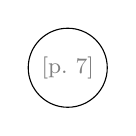
\begin{tikzpicture}
\node[draw,circle,inner sep=3pt] {\mspage{7}};
\end{tikzpicture}}

\diagram{\begin{tikzcd}[ampersand replacement=\&,column sep=1.6em,row sep=2.8em,column sep=9pt,row sep=14pt,execute at begin picture={\fontsize{10}{12}\selectfont}]
\&\&
\begin{gathered}
\widetilde\rho=(\rho_0,2)=(\rho,2)\\
\widetilde\sigma=(\sigma_0,3)=(\sigma,3)
\end{gathered}
\arrow[d, bend right=20]
\&
\begin{gathered}
\deleted{\unsure{\Pi_{0,3}^{D}}}\\[-2pt]
\inserted{\text{\uline{\unsure{identified with}}}}\\[-2pt]
\inserted{\unsure{S\mathcal T_{11}\times_{\Pi_{0,3}^{D}}\mathbb Z/12\mathbb Z}}
\end{gathered}
\arrow[d]
\&
\begin{gathered}
\rho_0=(\rho,\dot 2)\\[-2pt]
\unsure{\Pi_{0,3}}\\[-2pt]
\sigma_0=(\sigma,\dot 3)=(\sigma,-1)
\end{gathered}
\arrow[d]
\&\\
\unsure{0|1}\arrow[r,dash]\&
\mathbb Z\arrow[r,dash,"1\unsure{-|\mapsto}\overline\omega=\omega^2"]\arrow[dd,equal]\&
S\mathcal T_{11}\arrow[r,Rightarrow]\arrow[dd,"\substack{\widetilde\rho\mapsto\deleted{\unsure{4}}2\\\widetilde\sigma\mapsto3}"']
\arrow[ddr,phantom,"\text{Cartesian}"]\&
\mathcal T_{11}\arrow[r,Rightarrow]\arrow[dr,leftrightarrow]\arrow[dd,"\substack{\rho_0\mapsto\dot 2\\\sigma_0\mapsto\dot 3}"']
\&\Pi_{0,3}^{\prime D}\arrow[dr,"\text{canonical}"]\arrow[dd,"\substack{\rho\mapsto2\\\sigma\mapsto3}"{pos=.25,xshift=2pt}]
\arrow[dl,phantom,"\text{cartesian}" description]\&\\
\&\&\&{}\&
|[xshift=-3em]|\mathbb D'_3\arrow[r,"\text{cartesian}"{pos=.75}]\arrow[dd]
\&\mathbb D_3\arrow[dd,"\text{canonical}"]\\
1\arrow[r,dash]\&\mathbb Z\arrow[r,"12"]\&\mathbb Z\arrow[r,"\text{canonical}"]\&
\mathbb Z/12\mathbb Z\arrow[r,"\text{canonical}"]\arrow[dr,"\text{canonical}"']
\&\mathbb Z/6\mathbb Z\arrow[dr,"\text{canonical}"]
\arrow[d,phantom,"\text{\uline{Cartesian}}"'{pos=.25,xshift=-3em}]
\arrow[dr,phantom,"\text{\uline{cartesian}}"{description,xshift=-1.5em,yshift=.5em}]\&\\
\&\&\&\&\mathbb Z/4\mathbb Z\arrow[r,leftrightarrow,"\text{canonical}"]\&\mathbb Z/2\mathbb Z
\end{tikzcd}}

\margin{\unsure{for} $\mathcal T_{11}$ \unsure{identified with}
$\Pi_{0,3}^{D}\times_{\mathbb Z/2\mathbb Z}\mathbb Z/4\mathbb Z$}

\unsure{Have we} \unsure{indeed}\quad
$\bigm|\quad S\mathcal T_{11}\simeq S\Pi_{0,3}^{D}$ ??

it would rather seem, however
\[
\deleted{\unsure{\mathcal T_{11}}}\quad
PM_{11}\simeq
\left(\underbrace{T^*U_{0,3}}_{\substack{\text{bundle}\\\text{\uline{tangent}}}},\mathfrak S_3\right)
\]
\inserted{(and \uline{not} $\unsure{PU_{0,3}}$ !!)}

\[
\text{thus}\quad \mathcal T_{11}\simeq\pi_1(T^*U_{0,3},\mathfrak S_3)\ \ldots
\]
\margin{19}

\clearpage
\LMcote{140-1}
\typeout{LMLAYOUTSCAN 140-1 36}
\scanpage{36}
\diagram{\begin{tikzcd}[ampersand replacement=\&,column sep=large,row sep=large,column sep=9pt,row sep=14pt,execute at begin picture={\fontsize{10}{12}\selectfont}]
 \&\&\left\{\rho,\sigma\mid\underbrace{\rho^3=\sigma^2}_{\omega'^{-1}=\omega}\right\}\deleted{\unsure{\omega|\infty}}\arrow[d,equal]\&\&\\
 1\arrow[r,no head]\&\overset{\omega'=\unsure{\omega^{-1}|\overline\omega'}}{\mathbb Z}\arrow[r]\arrow[d,equal]\&S\Pi_{0,3}^D\arrow[r]\arrow[d]\&\Pi_{0,3}^D\arrow[r,no head]\arrow[d]\&1\\
 1\arrow[r,no head]\&\mathbb Z\arrow[r]\&S\Pi_{0,3}^D(4)\arrow[r]\&\Pi_{0,3}^D\times\mathbb Z/4\mathbb Z\arrow[r,no head]\&1\\[4em]
 1\arrow[r]\&\underset{\omega^2}{\mathbb Z}\arrow[r]\arrow[u,very thick]\&S\mathcal T_{11}\arrow[r]\arrow[u,very thick,"{\underbrace{\begin{gathered}\rho\mapsto\rho\overline\omega^2\\\sigma\mapsto\sigma\overline\omega^3\\\omega\longrightarrow\overline\omega^2\\\omega^2\longrightarrow\overline\omega^4=\omega'\end{gathered}}}"]\&\mathcal T_{11}\arrow[u,hook,"{\substack{\rho\mapsto(\rho,2)\\\sigma\mapsto(\sigma,3)}}"]\&\omega\longrightarrow(1,2)
\end{tikzcd}}
\margin{$S\Pi_{0,3}^D(4)=\left\{\rho,\sigma,\overline\omega\mid\begin{gathered}\rho^3=\sigma^2=\overline\omega^{-4}\\\overline\omega\ \text{central}\end{gathered}\right\}$\\
N.B. $\unsure{\dot{\overline\omega}|\overline\omega}^{4}=\unsure{\omega^{-1}}$\\
$=\omega'\deleted{\unsure{\omega}}$}

% Groupe et flèche au pied du feuillet, écrits tête-bêche.
\diagram{\begin{tikzcd}[ampersand replacement=\&,column sep=large]
 \overbrace{S\Pi_{0,3}^D(4)}^{\pi_1(U_{0,3},\mathfrak S_3\times\mu_4)}\arrow[r]\&\Pi_{0,3}^D
\end{tikzcd}}
\margin{35}

\clearpage
\LMcote{140-2}
\typeout{LMLAYOUTSCAN 140-2 302}
\scanpage{302}
\mspage{152}

tially to: determining the kernel of
\[
S\unsure{A|\mathcal A}_{g,\nu}/(SA_{g,\nu})^0\longrightarrow\Gamma^!_{g,\nu},
\quad\text{i.e.}\quad
SA_{g,\nu}\cap A_{g,\nu}^0/(SA_{g,\nu})^0
\]
as $T^I=T^{S_{g,\nu}}$. We can probably reduce to the context of \inserted{compact} surfaces with boundary (let us denote by a $'$ the corresponding topological groups), we have
\[
1\longrightarrow SA_{g,\nu}^{\prime+}\longrightarrow
A_{g,\nu}^{\prime!+}\longrightarrow
\prod_{i\in S_{g,\nu}}\operatorname{Aut}^+(C_i)\longrightarrow1
\]
\margin{homotopic to the standard \unsure{circle} \deleted{\illegible{1}} group $\mathbb U$, twisted by $\unsure{T|\Pi}$}
where the $+$ indicates the automorphisms preserving the \unsure{orientation}, and the $C_i$ are the connected components of the boundary. We conclude from this the homotopy exact sequence
\LMlayoutnotice{140-2-302-D1}
\begin{landscape}
\begin{center}
\begin{tikzcd}[ampersand replacement=\&,column sep=small,row sep=small,column sep=9pt,row sep=14pt,execute at begin picture={\fontsize{10}{12}\selectfont}]
\inserted{0=\unsure{\prod_i|\prod}\unsure{\Pi_2|\pi_2}(\operatorname{Aut}^+(C_i))}
\arrow[r] \&
\unsure{\Pi_1|\pi_1}(SA_{g,\nu}^{\prime0})\arrow[r] \&
\unsure{\Pi_1|\pi_1}(A_{g,\nu}^{\prime!+})\arrow[r]\arrow[d,equal] \&
\deleted{\unsure{\Pi_0}}\prod_i\unsure{\Pi_1|\pi_1}(\operatorname{Aut}^+(C_i))\arrow[r]\arrow[d,phantom,"\unsure{\wr}"] \&
\unsure{\Pi_0|\pi_0}(SA_{g,\nu}^{\prime+})\arrow[r] \&
\unsure{\Pi_0|\pi_0}(A_{g,\nu}^{\prime!+})\arrow[d,equal]\arrow[dd,bend left=28] \\
\&\&\unsure{\Pi_1|\pi_1}(A_{g,\nu}^{\prime0})\&\unsure{T^I}\&\overset{\uparrow}{\uline{\text{to be computed}}}\&\Gamma_{g,\nu}'\\
\&\&\&\&\&1=\prod_i\unsure{\Pi_0|\pi_0}(\operatorname{Aut}^+(C_i))
\end{tikzcd}\end{center}
\end{landscape}
\[
\left[\text{and}\quad
\unsure{\Pi_i|\pi_i}(SA'_{g,\nu})\xrightarrow{\sim}
\unsure{\Pi_i|\pi_i}(A_{g,\nu}^{\prime\unsure{0}})
\quad\text{if }i\geq2\right]
\]

i.e.
\[
\left\{\begin{aligned}
0&\longrightarrow\unsure{\Pi_1|\pi_1}(SA_{g,\nu}^{\prime+})
\longrightarrow\unsure{\Pi_1|\pi_1}(A_{g,\nu}^{\prime0})
\longrightarrow T^I\longrightarrow\unsure{\Pi_0|\pi_0}(SA_{g,\nu}^{\prime!+})
\longrightarrow\Gamma_{g,\nu}^{\prime!+}\longrightarrow1.\\
&\unsure{\Pi_i|\pi_i}(SA_{g,\nu}^{\prime+})\xrightarrow{\sim}
\deleted{\illegible{1}}\unsure{\Pi_i|\pi_i}(A_{g,\nu}^{\prime0})
\quad\text{for }i\geq2
\end{aligned}\right.
\]
\deleted{In the case \illegible{1}}

We have an obvious homomorphism: (by '\unsure{gluing} disks')
$A_{g,\nu}^{\prime\unsure{0}}\longrightarrow A_{g,\nu}$ inducing
$SA'_{g,\nu}\longrightarrow SA_{g,\nu}$,
\deleted{which} and these are surely homotopy equivalences, so
\deleted{\illegible{1}} the preceding exact sequence

\mspage{301}

\clearpage
\LMcote{140-2}
\typeout{LMLAYOUTSCAN 140-2 328}
\scanpage{328}
\mspage{\unsure{166|168}}

\[
\unsure{(\overline{21})|(\overline{21}')}\qquad
1\longrightarrow\pi\longrightarrow\pi_1(\unsure{U|\mathcal{U}}_{g,\nu\,\overline{Q}})
\longrightarrow\pi_1(M_{g,\nu\,\overline{Q}})\longrightarrow1
\]
\deleted{\(\unsure{(\overline{22})}\qquad 1\longrightarrow\pi\longrightarrow\)}

We of course have an \unsure{isomorphism} of groups with \unsure{loops|ends}
\[
(23)\qquad \pi\simeq\widehat{\Pi}_{g,\nu}
\]
whose indeterminacy we would like to determine precisely

Let $M_{g,\nu\,C}$ denote the complex modular Teichmüller \deleted{\illegible{1}}\inserted{topos}, defined using the \deleted{differentiable}\inserted{$C^\infty$} surface $\unsure{U|\mathcal{U}}_{g,\nu}$, it is equipped with the canonical universal covering $\widetilde{M}_{g,\nu\,C}$ (\S~21)
\margin{$\widetilde{M}_{g,\nu\,C}=E_g/\unsure{A_{g,\nu}^{0}|A_{g,\nu}^{\circ}}$}
with group \unsure{of automorphisms} $\mathcal{T}_{g,\nu}^{+}$ precisely \unsure{--|...}
$\unsure{U|\mathcal{U}}_{g,\nu\,C}$ being itself also equipped with a universal covering \unsure{over} the preceding one,
$\widetilde{\unsure{U|\mathcal{U}}}_{g,\nu\,C}=E_g/\unsure{A_{g,\nu+1}^{0}|A_{g,\nu+1}^{\circ}}$.
This gives rise to the exact sequence of discrete groups (in the general topology context)
\diagram{
\begin{tikzcd}[column sep=large,row sep=large,ampersand replacement=\&,column sep=9pt,row sep=14pt,execute at begin picture={\fontsize{10}{12}\selectfont}]
(24) \& 1 \arrow[r] \& \Pi_{g,\nu} \arrow[r] \arrow[dd] \& \unsure{\mathfrak{S}|\mathcal{G}}_{g,\nu}^{+} \arrow[r] \arrow[d,equal] \& \mathcal{T}_{g,\nu}^{+} \arrow[r] \arrow[d,equal] \& 1 \\
\& \& \& \pi_1(\unsure{U|\mathcal{U}}_{g,\nu\,C}) \arrow[d] \& \pi_1(M_{g,\nu\,C}) \arrow[d] \& \\
\text{(mapping to} \& 1 \arrow[r] \& \Pi_{g,\nu} \arrow[r] \& \operatorname{Aut}_{\mathrm{lac}}\deleted{\unsure{\mathrm{ext}}}(\Pi_{g,\nu}) \arrow[r] \arrow[d,equal] \& \operatorname{Aut\,ext}_{\mathrm{lac}}(\Pi_{g,\nu}) \arrow[r] \arrow[d,equal] \& 1 \\
\& \& \& \unsure{\mathfrak{S}|\mathcal{G}}_{g,\nu} \& \mathcal{T}_{g,\nu} \&
\end{tikzcd}
}
by an \unsure{isomorphism|homomorphism} of extension \unsure{structures}), which by passage to the profinite completions gives the analogous exact sequence for the

\mspage{327}

\clearpage
\LMcote{140-2}
\typeout{LMLAYOUTSCAN 140-2 331}
\scanpage{331}

is canonically endowed (not with a discrete \inserted{oriented} quasi-rigidification, which depends on the choice of an isomorphism $\overline{\mathbb Q}\simeq\overline{\mathbb Q}_0$ i.e. of an embedding $\overline{\mathbb Q}\subset\mathbb C$) but at least with a strict geometric Teichmüller group $\Sigma\subset\widehat{\widehat{\mathcal T}}(\pi)$, namely the image of $\pi_1(M_{g,\nu\overline{\mathbb Q}})$, \inserted{isomorphic to} This being so, We have a canonical homomorphism of group extensions

\diagram{(26)\quad
\begin{tikzcd}[ampersand replacement=\&, column sep=small,column sep=9pt,row sep=14pt,execute at begin picture={\fontsize{10}{12}\selectfont}]
1 \arrow[r] \&
\pi_1(M_{g,\nu\overline{\mathbb Q}}) \arrow[r] \arrow[d, "{\unsure{\wr|2}}"] \&
\pi_1(M_{g,\nu}) \arrow[r, no head] \arrow[d] \&
\operatorname{Gal}(\overline{\mathbb Q}/\mathbb Q) \arrow[r] \arrow[d] \&
1 \\
1 \arrow[r] \&
\Sigma \arrow[r] \&
\unsure{\mathcal N|N}_\Sigma \arrow[r] \arrow[d, equal] \&
\Gamma_\Sigma \arrow[r] \arrow[dr] \&
1 \\
\& \&
\operatorname{Norm}_{\widehat{\widehat{\mathcal T}}(\pi)}(\Sigma) \&
\&
\text{\parbox[t]{105pt}{\footnotesize\rule{28pt}{.3pt}\\\textit{\LMnotelabel.}\enspace \margin{group of \deleted{\unsure{``arithmetic}}\inserted{outer} ``arithmetic'' automorphisms of $\pi$ (endowed with $\Sigma$)}}}
\end{tikzcd}}

For the choice of an isomorphism $\overline{\mathbb Q}\simeq\overline{\mathbb Q}_0$ i.e. of an embedding $\overline{\mathbb Q}\subset\mathbb C$, the image of complex conjugation in $\operatorname{Gal}(\overline{\mathbb Q}_0/\mathbb Q)$ is none other than \unsure{the element} of order $2$ of $\Gamma_\Sigma$ associated with the geometric Teichmüller subgroup, associated with the canonical quasi-discretification (oriented, but no matter) on $\pi$ (defined by $\overline{\mathbb Q}\unsure{\simeq|\xrightarrow{\sim}}\overline{\mathbb Q}_0$).

\clearpage
\LMcote{140-2}
\typeout{LMLAYOUTSCAN 140-2 344}
\scanpage{344}
\mspage{174}

\LMlayoutnotice{140-2-344-D1}
\begin{landscape}
\begin{center}
\begin{tikzcd}[ampersand replacement=\&,column sep=large,row sep=large,column sep=9pt,row sep=9pt,execute at begin picture={\fontsize{9}{11}\selectfont}]
\& \&
\begin{gathered}
\text{Bases of }(\pi)\simeq\operatorname{Isom}_{\mathrm{lac}}(\widehat{\pi}_{g,\nu},\pi)\\
\downarrow\\
[\text{Bases}^{!}(\pi)\simeq\operatorname{Isom}^{!}_{\mathrm{lac}}(\widehat{\pi}_{g,\nu},\pi)]
\end{gathered}
\arrow[dl,"\mathcal G^{+}_{g,\nu}"']\arrow[dr,"\widehat{\pi}_{g,\nu}"]
\&\\
\&
\begin{gathered}
\text{discretifications}\ \inserted{\text{oriented}}\ (\pi)\\
\simeq\operatorname{Isom}_{\mathrm{lac}}(\widehat{\pi}_{g,\nu},\pi)/\mathcal G^{+}_{g,\nu}\\
\simeq\operatorname{Isom}^{!}_{\mathrm{lac}}(\widehat{\pi}_{g,\nu},\pi)/\mathcal G^{!+}_{g,\nu}
\end{gathered}
\arrow[dl,"\{\pm1\}"']\arrow[dr]
\&\&
\begin{gathered}
\text{Outer bases of }\pi\\
\simeq\operatorname{Isom}\deleted{\,\mathrm{ext}}_{\mathrm{lac}}(\widehat{\pi}_{g,\nu},\pi)/\widehat{\pi}_{g,\nu}\\
\simeq\operatorname{Isom\,ext}_{\mathrm{lac}}(\widehat{\pi}_{g,\nu},\pi)\\
\downarrow\\
[\text{Outer bases}^{!}(\pi)\simeq\operatorname{Isom\,ext}^{!}_{\mathrm{lac}}(\widehat{\pi}_{g,\nu},\pi)]
\end{gathered}
\arrow[dl,"\mathcal T_{g,\nu}"]\\
\left[\begin{gathered}\text{Discretifications }(\pi)\\\simeq\end{gathered}\right]
\arrow[d]
\&\&
\begin{gathered}
\text{prediscretifications}\ \inserted{\text{oriented}}\ \text{strict}\ (\pi)\\
\simeq\operatorname{Isom}_{\mathrm{lac}}(\unsure{\widehat{\pi}}_{g,\nu},\pi)/\mathcal G^{+}_{g,\nu}\cdot\widehat{\pi}_{g,\nu}\\
\simeq\operatorname{Isom\,ext}_{\mathrm{lac}}(\widehat{\pi}_{g,\nu},\pi)/\mathcal T^{+}_{g,\nu})\\
\simeq\operatorname{Isom}^{!}(\widehat{\pi}_{g,\nu},\pi)/\mathcal G^{!+}_{g,\nu}\cdot\widehat{\pi}_{g,\nu}\\
\simeq\operatorname{Isom\,ext}_{\mathrm{lac}}(\widehat{\pi}_{g,\nu},\pi)/\mathcal T^{!+}_{g,\nu}
\end{gathered}
\arrow[dll,"\{\pm1\}"']\arrow[d]
\&\\
\left[\begin{gathered}\text{strict prediscretifications}\\\text{of }\pi\\\simeq\end{gathered}\right]
\&\&
\begin{gathered}
\text{prediscretifications}\ \inserted{\text{oriented}}\ (\pi)\\
\simeq\operatorname{Isom}_{\mathrm{lac}}(\widehat{\pi}_{g,\nu},\pi)/\widehat{\mathcal G}^{+}_{g,\nu}\\
\simeq\operatorname{Isom\,ext}_{\mathrm{lac}}(\widehat{\pi}_{g,\nu},\pi)/\widehat{\mathcal T}^{+}_{g,\nu}\\
\deleted{\unsure{\simeq}}\quad
\simeq\operatorname{Isom}^{!}_{\mathrm{lac}}(\widehat{\pi}_{g,\nu},\pi)/\widehat{\mathcal G}^{!+}_{g,\nu}\\
\simeq\operatorname{Isom\,ext}^{!}_{\mathrm{lac}}(\widehat{\pi}_{g,\nu},\pi)/\widehat{\mathcal T}^{!+}_{g,\nu}
\end{gathered}
\arrow[dll,"\{\pm1\}"']\arrow[dd,"\Gamma_{\Sigma}"',"\Gamma_{g,\nu}"]
\&\\
\left[\begin{gathered}\text{prediscretifications of }\pi\\\simeq\end{gathered}\right]
\arrow[drr]
\&\&\&\\
\&\&
\begin{gathered}
\text{prearithmetizations of }\pi\\
\simeq\operatorname{Isom}_{\mathrm{lac}}(\widehat{\pi}_{g,\nu},\pi)/\mathcal M_{g,\nu}\\
\simeq\operatorname{Isom\,ext}_{\mathrm{lac}}(\widehat{\pi}_{g,\nu},\pi)/\mathcal N_{g,\nu}\\
\simeq\operatorname{Isom}^{!}_{\mathrm{lac}}(\widehat{\pi}_{g,\nu},\pi)/\mathcal M^{!}_{g,\nu}\\
\simeq\operatorname{Isom\,ext}^{!}_{\mathrm{lac}}(\widehat{\pi}_{g,\nu},\pi)/\mathcal N^{!}_{g,\nu}
\end{gathered}
\&
\end{tikzcd}\end{center}
\end{landscape}

\margin{\unsure{not separated}}
\margin{\unsure{not separated}}
\margin{\diagram{\begin{tikzcd}[ampersand replacement=\&]
\deleted{\left\downarrow\vphantom{\rule{0pt}{2.8cm}}\right.}
\end{tikzcd}}}
\margin{\diagram{\begin{tikzcd}[ampersand replacement=\&,column sep=0.35cm,row sep=1.4cm,cells={nodes={inner sep=0pt,minimum size=0pt}}]
{} \& {} \arrow[d,bend right=8,line width=0.8pt,
  "{\widehat{\mathcal T}_{g,\nu}}"{pos=0.95,right}] \\
{} \& {} \arrow[dl,bend right=8,no head,line width=0.3pt] \\
{} \& {}
\end{tikzcd}}}
\margin{\diagram{\begin{tikzcd}[ampersand replacement=\&,column sep=0.30cm,row sep=0.40cm,cells={nodes={inner sep=0pt,minimum size=0pt}},arrows={line width=0.65pt,start anchor=center,end anchor=center,shorten <=1.2pt,shorten >=1.2pt}]
{} \& {} \& {} \arrow[dl] \arrow[dr] \& {} \& {} \arrow[ll] \arrow[dr] \& {} \\
|[yshift=-0.05cm]| {} \arrow[dr] \& {} \arrow[l] \arrow[dr] \& {} \& {} \arrow[dl] \& {} \& {} \arrow[ll] \\
{} \& |[yshift=-0.04cm]| {} \arrow[d] \& {} \arrow[l] \arrow[d] \& {} \& {} \& {} \\
{} \& |[yshift=-0.06cm]| {} \arrow[dr] \& {} \arrow[l] \arrow[dd,line width=1.25pt] \& {} \& {} \& {} \\
{} \& {} \& |[xshift=-0.12cm,yshift=-0.25cm]| {} \& {} \& {} \& {} \\
{} \& {} \& |[yshift=-0.45cm]| {} \& {} \& {} \& {}
\end{tikzcd}}}
\margin{Please turn over}
\mspage{343}

\clearpage
\LMcote{140-2}
\typeout{LMLAYOUTSCAN 140-2 346}
\scanpage{346}
\mspage{175}

We observe that, with the exception of the two homogeneous spaces
(under $\widehat{\widehat{\mathcal G}}(\pi)$, but not \unsure{necessarily|necessarily} under
$\widehat{\widehat{\mathcal G}}(\pi,I')$, or even under
$\widehat{\widehat{\mathcal G}}^{!}(\pi)$) Bases $(\pi)$ and Outer bases $(\pi)$,
the other four are in fact homogeneous spaces under
$\widehat{\widehat{\mathcal G}}^{!}$, and are expressed as quotients of the
\inserted{$\widehat{\widehat{\mathcal G}}^{!}_{g,\nu}$-}torsor
$\operatorname{Isom}^{!}(\widehat{\pi}_{g,\nu},\pi)$, by the four subgroups
\[
\mathcal G^{!}_{g,\nu},\quad
\mathcal G^{!}_{g,\nu}\cdot\widehat{\pi}_{g,\nu},\quad
\widehat{\mathcal G}^{!}_{g,\nu},\quad
\mathcal M^{!}_{g,\nu}
\]
(the last defined as the inverse image of $\mathcal N^{!}_{g,\nu}$ in
$\widehat{\widehat{\mathcal G}}_{g,\nu}$, just as $\mathcal M_{g,\nu}$ is defined
as the inverse image of $\mathcal N_{g,\nu}$).
We find on the other hand, \unsure{if|for} $I'=\{i_0,\ldots,i_{\nu'-1}\}$,
\unsure{a|some} homomorphism
\[
\widehat{\widehat{\mathcal G}}^{!}_{g,\nu}\longrightarrow
\widehat{\widehat{\mathcal G}}^{!}_{g,\nu'},
\]
sending $\mathcal G^{!}_{g,\nu}$ into $\mathcal G^{!}_{g,\nu'}$,
\deleted{\illegible{1} $\unsure{\widehat{\mathcal G}}_{g,\nu}$ into
$\unsure{\widehat{\pi}_{g,\nu}}$}
by sending $\pi_{g,\nu}$ into $\pi_{g,\nu'}$, thus $\widehat{\pi}_{g,\nu}$
into $\widehat{\pi}_{g,\nu'}$,
$\widehat{\mathcal G}^{!}_{g,\nu}=\Sigma^{!}_{g,\nu}$ into
$\widehat{\mathcal G}^{!}_{g,\nu'}=\Sigma^{!}_{g,\nu'}$, and the subgroup
$\mathcal G^{!}_{g,\nu}\cdot\widehat{\pi}_{g,\nu}$ of
\deleted{\illegible{1}} \inserted{$\widehat{\mathcal G}^{!}_{g,\nu}$}
into the subgroup $\mathcal G^{!}_{g,\nu'}\cdot\widehat{\pi}_{g,\nu'}$ of
$\widehat{\mathcal G}^{!}_{g,\nu'}$.
Finally, since $\Sigma^{!}_{g,\nu}$ maps into $\Sigma^{!}_{g,\nu'}$,
\deleted{\illegible{1}} $\mathcal N^{!}_{g,\nu}$ maps into the normalizer
of $\Sigma^{!}_{g,\nu'}$ \inserted{(in $\widehat{\widehat{\mathcal T}}^{!}_{g,\nu'}$)},
\deleted{which}\inserted{I say that this} is none other than $\mathcal N^{!}_{g,\nu'}$.
Changing notation, this amounts to the

\uline{Lemma}\quad The
$\mathcal N^{!}_{\Sigma}=\operatorname{Norm}_{\widehat{\widehat{\mathcal T}}^{!}}(\Sigma^{!})$
\deleted{\illegible{1}}
$\bigl(=\operatorname{Norm}_{\widehat{\widehat{\mathcal T}}}(\Sigma^{!})\cap
\widehat{\widehat{\mathcal T}}^{!}\bigr)$.

\margin{not proved\quad
\deleted{\illegible{4} of
$\unsure{\operatorname{Norm}_{\widehat{\widehat{\mathcal T}}}(\Sigma^{!})/\Sigma^{!}}$}}

Obviously we have
$\mathcal N^{!}_{\Sigma}\subset
\operatorname{Norm}_{\widehat{\widehat{\mathcal T}}}(\Sigma^{!})\cap
\widehat{\widehat{\mathcal T}}^{!}$,
conversely let $g\in\widehat{\widehat{\mathcal T}}^{!}$ which normalizes
$\unsure{\Sigma^{!}}$, let us show that it normalizes $\Sigma$ i.e.
that it \unsure{is} $\in\mathcal N$
(thus $\in\mathcal N^{!}=\mathcal N\cap\widehat{\widehat{\mathcal T}}^{!}$).
\mspage{345}

\clearpage
\LMcote{140-2}
\typeout{LMLAYOUTSCAN 140-2 348}
\scanpage{348}
\mspage{176}

i.e. $\widehat{\widehat{\mathcal G}}(\pi,i)\longrightarrow
\widehat{\widehat{\mathcal G}}(\pi')$ is trivial on $\unsure{\widehat{\pi}}$, and
thus passes to the quotient as a
$\widehat{\widehat{\mathcal T}}(\pi,i)\longrightarrow
\widehat{\widehat{\mathcal G}}(\pi,i)$.
I assume, \deleted{that} by analogy with the discrete case,
that this homomorphism is an \uline{isomorphism}, so that we have an exact sequence
\margin{\figure{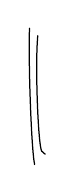
\begin{tikzpicture}[x=1cm,y=1cm,line width=.45pt,line cap=round]
\draw (0,0) .. controls (-.015,-.48) and (.025,-1.54) .. (.065,-1.73);
\draw (.105,-.095) .. controls (.070,-.48) and (.110,-1.48) .. (.155,-1.56) .. controls (.165,-1.58) and (.185,-1.59) .. (.200,-1.60);
\end{tikzpicture}}}
\margin{\unsure{recall that we assume} $\pi$ \unsure{anabelian|nonabelian}
$(2g+\nu\geq3)$}
\[
1\longrightarrow\pi'\longrightarrow
\widehat{\widehat{\mathcal T}}(\pi,i)\longrightarrow
\unsure{\widehat{\widehat{\mathcal G}}}(\pi',i)\longrightarrow1
\]
or again
\[
1\longrightarrow\widehat{\pi}_{g,\nu-1}\longrightarrow
\widehat{\widehat{\mathcal T}}_{g,(\nu,\nu-1)}
\longrightarrow\unsure{\widehat{\widehat{\mathcal G}}}_{g,\nu-1}
\longrightarrow1
\]
which contains the exact sequence
\[
1\longrightarrow\pi_{g,\nu-1}^{\unsure{*|+}}\longrightarrow
\mathcal T_{g,(\nu,\nu-1)}\longrightarrow
\unsure{\mathcal G}_{g,\nu-1}\longrightarrow1
\]
\unsure{as|known} sub\deleted{\unsure{particular|dense part}}, \unsure{sequence|is} exact.
It is convenient to work instead with
\diagram{\begin{tikzcd}[ampersand replacement=\&,column sep=2.1em,row sep=3.0em]
1 \arrow[r,dash] \&
\pi_{g,\nu-1} \arrow[r,dash] \arrow[d,hook',no head] \&
\unsure{\mathcal T}_{g,\nu}^{!+} \arrow[r] \arrow[d,hook',no head] \&
\mathcal G_{g,\nu-1}^{!+} \arrow[r,dash] \arrow[d,hook',no head] \& 1 \\
1 \arrow[r,dash] \&
\widehat{\pi}_{g,\nu-1} \arrow[r] \arrow[d,equal] \&
\underset{\deleted{\unsure{\illegible{1}}}}{\widehat{\mathcal T}_{g,\nu}^{!+}}
\arrow[r] \arrow[d,hook',no head] \&
\widehat{\mathcal G}_{g,\nu-1}^{!+} \arrow[r,dash] \arrow[d,hook'] \& 1 \\
1 \arrow[r,dash] \&
\widehat{\pi}_{g,\nu-1} \arrow[r] \&
\widehat{\widehat{\mathcal T}}_{g,\nu}^{!} \arrow[r] \&
\widehat{\widehat{\mathcal G}}_{g,\nu-1}^{!} \arrow[r,dash] \& 1
\end{tikzcd}}

The map \LMmathnotice{140-2-348-M1}
\begin{multline*}\unsure{\text{Prediscretifications}|\text{Prediscretifications}}^{+}(\pi)\\\longrightarrow
\unsure{\text{Prediscretifications}|\text{Prediscretifications}}^{+}(\pi')\end{multline*} is thus identified with
$\widehat{\widehat{\mathcal T}}_{g,\nu}^{!}/\widehat{\mathcal T}_{g,\nu}^{!}$,
we read off the diagram that this is
$\simeq\widehat{\widehat{\mathcal G}}_{g,\nu-1}^{\unsure{!}\deleted{\unsure{+}}}/
\widehat{\mathcal G}_{g,\nu-1}^{!+}$,
whence bijectivity on the sets of oriented prediscretifications.

In the group $\widehat{\widehat{\mathcal T}}_{g,\nu}^{!}=\mathcal T$,
we have an invariant subgroup $\widehat{\pi}_{g,\nu-1}=\pi'$,
and a subgroup $\Sigma$ $(\unsure{=|\longleftarrow}\widehat{\mathcal T}_{g,\nu}^{!+})$
\mspage{347}

\clearpage
\LMcote{140-2}
\typeout{LMLAYOUTSCAN 140-2 384}
\scanpage{384}

property by saying that there exists a \unsure{discretification} \inserted{$\pi_0$} of $\pi$, compatible with $a$, such that $Z\subset\mathcal T(\pi_0)$\ldots)

\unsure{Let us consider} now an arbitrary finite subgroup $G\subset\widehat{\mathcal T}_a^+$. [N.B. If we take \inserted{only} $G\subset M_a$, so that the image of $G$ in $\mathbb{\Gamma}_a=M_a/\widehat{\mathcal T}_a^+$ is a finite subgroup, then if it \deleted{$\mathbb{\Gamma}_a$} is true that $\mathbb{\Gamma}_a\simeq\unsure{\mathcal G|\mathfrak G}$, \margin{$\operatorname{Gal}(\overline{\mathbb Q}/\mathbb Q)\longrightarrow$} this image must be of order $1$ or $2$, and in the second case must \margin{\unsure{?}} define a $\tau\in\mathbb{\Gamma}_a$ corresponding to a well-determined \uline{\unsure{prediscretification}} (not oriented) of $\pi$. This case should be reused again in what follows\ldots]. \deleted{If we} \inserted{Let us suppose, \unsure{or}} \unsure{admit}, that $G$ is contained in $\mathcal T^+$, \margin{this is probably \uline{not} automatic (if we \unsure{do} \unsure{not|N'} suppose $N_a=\operatorname{Norm}_{\widehat{\widehat{\mathcal T}}}(\unsure{\widehat{\mathcal T}_a|\widehat{\mathcal T}_a^+})$)} for a suitable discretification in the class $a$, and that the outer action of $G$ thus obtained on a discrete $\pi_0$ of type $(g,\nu)$ \unsure{is|are} always \uline{realizable}. It is therefore also realizable \unsure{by|for} an action of $G$

\clearpage
\LMcote{140-2}
\typeout{LMLAYOUTSCAN 140-2 411}
\scanpage{411}
\mspage{208}

and unless I am mistaken, it has become obvious
that this functor is an \uline{equivalence of
categories} (and as a consequence, there
\margin{\unsure{for the} \uline{\unsure{isomorphisms}}}
is the functor in the opposite direction :
drill holes at ``points'' invariant
under $\Gamma_{\unsure{a|0}}$ (or at arbitrary points,
at the cost of passing to a smaller $\Gamma'$).

But I realize that
\deleted{\illegible{1}} this is not at all obvious -- I am going
to try to elucidate the situation axiomatically.
We have fixed a genus $g$,
we suppose given, for varying $\nu$
(such that $(g,\nu)$ anabelian) closed
subgroups $N_{g,\nu}\subset\widehat{\widehat{\mathcal T}}_{g,\nu}$,
normalizing $\widehat{\mathcal T}_{g,\nu}$, and satisfying the
essential condition that the $\psi_i:\widehat{\widehat{\mathcal T}}_{g,\nu}\longrightarrow\widehat{\widehat{\unsure{\mathcal G|\mathcal S}}}_{g,\nu-1}$
induce
\[
M_{g,\nu}\xrightarrow{\sim}M_{g,\nu-1}
\]
Which makes it possible to define the notion
of arithmetization of a profinite $\pi$ of
anabelian type $(g,\nu)$, and the theory of

\clearpage
\LMcote{140-2}
\typeout{LMLAYOUTSCAN 140-2 419}
\scanpage{419}
\mspage{212}

Thanks to this, the equivalence of categories between systems
$(\pi,a,i,\Gamma,\unsure{\theta}:\Gamma\mathop{\longrightarrow}\limits_{\unsure{\mathrm{adm}}}\unsure{N_a})$,
and the systems $(\pi',a',\Gamma,\theta':\Gamma\longrightarrow\unsure{N_{a'}},P)$,
where $P\in\mathrm{Pt}(B_{\pi',\Gamma^{\natural}})^\Gamma$,
becomes perfectly precise at the level of points: the
$\Gamma$-rational Points of $B_{\pi\unsure{,\Gamma^{\natural}|\deleted{,\Gamma^{\natural}}}}$
are identified with \unsure{one|the set}
\deleted{of the $\Gamma$-\unsure{rational} points} of the $\Gamma$-rational points
of $B_{\pi'}$, distinct from $P$.

This then allows us (which was not feasible in the discrete
context!) to extend the equivalence of categories to an equivalence

\[
\begin{gathered}(30)\\[3pt]
\begin{array}{c@{\,}c@{\,}c}
\parbox[t]{0.44\linewidth}{%
category of systems $(\pi,\unsure{a|\alpha},I',\allowbreak\Gamma,\allowbreak\theta:\Gamma\longrightarrow N_a)$
of an arithmetized $\pi$ \inserted{(by \unsure{$\alpha$|$a$})} of type $(g,\nu)$,
of $I'\subset I(\pi)$, of an
\uline{admissible} outer action of $\Gamma$ on $\pi$
such that $\Gamma$ \deleted{\unsure{operates}} \uline{fixes each point} of $I'$
}
& \unsure{\cong|\simeq} &
\parbox[t]{0.44\linewidth}{%
category of systems
$(\pi',\unsure{a'|\alpha'},I',\allowbreak\unsure{\Gamma^{*}|\Gamma},\allowbreak\theta':\Gamma\longrightarrow N_{a'})$
of an arithmetized $\pi'$ (by \unsure{$a'$|$\alpha'$}) of type
$(g,\nu')$ $[\nu'=\nu-\mathrm{card}(I')]$
with an admissible \inserted{outer} operation of $\Gamma$ on it, and
a subset $I'\subset\mathrm{Pt}_{ad}(B_{\pi',\unsure{\Gamma}}\unsure{)}$
(hence $I'\subset\mathrm{Pt}_{ad}(B_{\pi',\Gamma})^\Gamma$)
i.e. $I'$ formed of points \unsure{invariant|fixed} under $\Gamma$, i.e. ``$\Gamma$-rational''
}
\end{array}
\end{gathered}\]

\margin{with $2g+(\underbrace{\nu-\mathrm{card}\,I'}_{\nu'})\geq3$}

We thus have a quasi-inverse functor:
drilling holes at $I'$ !

\clearpage
\LMcote{140-2}
\typeout{LMLAYOUTSCAN 140-2 508}
\scanpage{508}
\mspage{\unsure{258 (259)}}

map determined on $X$ by the spherical triangles $(0,1,\infty)$
(on the real axis as equator) -- which is thus the universal
\unsure{weighted} triangular map -- as the inverse image of the universal map
(having a single vertex $0$, a single edge (folded) $0\longrightarrow1$,
a single face, with center $\infty$).
\margin{\figure{\begin{tikzpicture}[x=1cm,y=1cm,line cap=round,line join=round]
\draw[line width=.45pt] (0,2.85)
 .. controls (-.71,2.83) and (-1.02,2.47) .. (-1,2)
 .. controls (-1.01,1.48) and (-.57,1.16) .. (0,1.15);
\draw[line width=.45pt] (0,2.85)
 .. controls (.76,2.85) and (1.03,2.48) .. (1,2.10);
\draw[line width=.45pt] (.99,1.98)
 .. controls (.98,1.62) and (.74,1.36) .. (.54,1.26);
\draw[line width=.5pt] (-1,2)
 .. controls (-.91,1.75) and (.83,1.74) .. (1,1.95);
\draw[densely dotted,line width=.65pt] (-1,2)
 .. controls (-.61,2.17) and (.63,2.17) .. (1,2.02);
\fill (0,2.85) circle (1.4pt);
\node[anchor=south west,inner sep=2pt] at (0,2.88) {$P=\unsure{-\bar j|-j}$};
\fill (0,1.15) circle (1.4pt);
\node[anchor=north west,inner sep=2pt] at (-.03,1.12) {$P'=\unsure{-j|-\bar j}$};
\fill (-.57,1.80) circle (1.4pt);
\node[below,inner sep=2pt] at (-.57,1.80) {$0$};
\fill (.78,1.82) circle (1.4pt);
\node[below,inner sep=2pt] at (.78,1.82) {$1$};
\fill (0,2.12) circle (1.5pt);
\node[above,inner sep=2pt] at (0,2.12) {$\infty$};
\draw[->,line width=.65pt] (-1.40,1.60)
 .. controls (-1.40,1.22) and (-1.38,.85) .. (-1.37,.58);
\draw[line width=.45pt] (.02,.48)
 .. controls (-.55,.48) and (-.86,.17) .. (-.82,-.20)
 .. controls (-.78,-.70) and (-.46,-1.02) .. (.10,-1.04);
\draw[line width=.45pt] (.02,.48)
 .. controls (.65,.46) and (.87,.12) .. (.82,-.29)
 .. controls (.81,-.58) and (.66,-.79) .. (.53,-.87);
\fill (.02,.48) circle (1.5pt);
\node[anchor=west,inner sep=2pt] at (.07,.48) {$\unsure{Q}(=P)$};
\fill (-.82,-.12) circle (1.5pt);
\node[left,inner sep=2pt] at (-.82,-.12) {$\infty$};
\fill (-.08,.10) circle (1.7pt);
\node[below,inner sep=2pt] at (-.08,.10) {$1$};
\fill (-.40,-.36) circle (1.7pt);
\node[below,inner sep=2pt] at (-.40,-.36) {$0$};
\draw[line width=1.15pt] (-.08,.10)
 .. controls (.28,.10) and (.71,.02) .. (.82,-.20)
 .. controls (.66,-.43) and (.03,-.47) .. (-.40,-.36);
\draw[densely dotted,line width=.65pt] (-.82,-.12)
 .. controls (-.60,.08) and (-.36,.08) .. (-.08,.10);
\draw[densely dotted,line width=.65pt] (-.82,-.12)
 .. controls (-.78,-.32) and (-.59,-.35) .. (-.40,-.36);
\node[below,inner sep=1pt] at (.22,-.44) {$\unsure{\varphi}$};
\end{tikzpicture}}}
Every topological \deleted{\unsure{of}} \inserted{étale} covering of
$U_{03}(\mathbb C)\subset X$ thus gives a topological étale covering of
$U_{0,3}(\mathbb C)\subset Y$, \deleted{ramified} having
\deleted{\illegible{1}} \inserted{over} $1$ ramification $2$,
over $\infty$ ramification $3$ \unsure{exactly|exactly},
which corresponds to the ``forgetful'' functor \inserted{(of the weighting)},
where a \unsure{weighted} triangular map is considered as
just a map. From the point of view of fundamental groups \unsure{we} thus find
an \deleted{\unsure{homomorphism} of outer groups}
\inserted{equivalence of categories}

\diagram{\begin{tikzcd}[ampersand replacement=\&,column sep=large,row sep=huge,column sep=9pt,row sep=14pt,execute at begin picture={\fontsize{10}{12}\selectfont}]
\&
\deleted{\begin{gathered}
\Pi_1(\unsure{X(\mathbb C)}\setminus\{0,1,\infty\})\\[-2pt]
\rotatebox{90}{$=$}\\[-2pt]
\Pi_{0,3}
\end{gathered}}
\arrow[r,phantom,"{\deleted{\longleftarrow}}" description]
\&
\deleted{\begin{gathered}
\Pi_1\!\left(Y(\mathbb C)\setminus\{0,1,\infty\};
\underbrace{2\{1\}+3\{\infty\}}_{\substack{\text{signature of}\\\text{ramification}}}\right)\\[-2pt]
\rotatebox{90}{$=$}\\[-2pt]
\Pi'_{0,3}
\end{gathered}}
\\
(\deleted{\illegible{1}}\inserted{4}) \&
\left(\text{Étale coverings of }X\setminus\{0,1,\infty\}=U_{0,3}\right)
\arrow[r,phantom,"\simeq" description]
\arrow[d,phantom,"{\rotatebox{-90}{$\simeq$}}" description]
\&
\begin{gathered}
\left[\begin{gathered}
\text{Coverings of }Y\setminus\{0,1,\infty\}=U_{0,3}\\
\text{with ramification subordinate to}\\
\text{the signature }2\{1\}+3\{\infty\}
\end{gathered}\right]\\
\big/\begin{gathered}
\text{the object }(X\setminus\{0,1,\infty\})\\
\text{of the said category}
\end{gathered}
\end{gathered}
\arrow[d,phantom,"{\rotatebox{90}{$\simeq$}}" description]
\\
\& \Pi_{0,3}\text{-sets} \&
(\Pi'_{0,3}\text{-Sets})/\deleted{\unsure{E}}E
\end{tikzcd}}

where $E$ is the $\Pi'_{0,3}$-set corresponding to the object
$X\setminus\{0,1,\infty\}$ of the category of étale coverings of
$\unsure{Y\setminus\{0,1,\infty\}}$ with ramification
\deleted{\unsure{imposed}}\inserted{\unsure{subordin-}}ate to
$2\{1\}+3\{\infty\}$

\deleted{$\unsure{\simeq}\ \unsure{\Pi_{0,3}^{\prime\circ}}\in\mathrm{Ens}$}

\clearpage
\LMcote{140-2}
\typeout{LMLAYOUTSCAN 140-2 512}
\scanpage{512}

above extend to this setting, and thus provide a homomorphism \deleted{outer} \inserted{of extensions}
\diagram{\begin{tikzcd}[ampersand replacement=\&]
1 \arrow[r] \& \widehat{\Pi}_{03} \arrow[r] \arrow[d] \& \mathcal E_{03} \arrow[r] \arrow[d] \& \Gamma \arrow[r] \arrow[d,equal] \& 1 \\
1 \arrow[r] \& \widehat{\Pi}'_{03} \arrow[r] \& \mathcal E'_{03} \arrow[r] \& \Gamma \arrow[r] \& 1
\end{tikzcd}\quad(9)},
modulo conjugation by an inner automorphism of $\Pi'_{03}$.

\margin{(9 bis) $\widehat{\Pi}_{0,3}\longrightarrow\widehat{\Pi}'_{0,3}$ fits into an exact sequence
\[
\boxed{1\longrightarrow\widehat{\Pi}_{0,3}\longrightarrow\widehat{\Pi}'_{0,3}\longrightarrow\unsure{\mathfrak S}_3\longrightarrow1}
\]
and ditto for the discrete groups
\[
\boxed{1\longrightarrow\Pi_{0,3}\longrightarrow\Pi'_{0,3}\longrightarrow\unsure{\mathfrak S}_3\longrightarrow1}.
\]}

That said, let $K$ be the kernel of the outer operation of $\Gamma$ on $\Pi'_{03}$. One then sees that \deleted{$K$ operates} the outer operation of $K$ on the open subgroup $\widehat{\Pi}_{03}$ takes place through a finite group (in fact, through \inserted{the intermediary of} $\widehat{\Pi}'_{03}/\widehat{\Pi}_{03}\simeq\unsure{\mathfrak S}_3$ \ldots) -- which implies, by theorem 1 of the \S\ above, that the group $K$ itself is finite. Thus by Artin one has $K=1$ or $K=(1,\tau)$, $\tau$ complex conjugation. But since $\chi(\tau)=-1$ it is obvious that the outer operation of $\tau$ on $\Pi'_{03}$ \inserted{(nor even on $(\Pi'_{03})_{\unsure{\mathrm{ab}}}^{*}$ \deleted{\illegible{2}})} is not trivial\ldots
\margin{$*\simeq\unsure{\mathbb Z/2\mathbb Z+\mathbb Z/3\mathbb Z}$}
\deleted{\unsure{Which}} This proves the proposition.

\clearpage
\LMcote{140-2}
\typeout{LMLAYOUTSCAN 140-2 527}
\scanpage{527}
\mspage{269}

It is \unsure{true} that it is well \unsure{known} that a cohomology class (37) with torsion coefficients is killed, on \unsure{passing} to a finite extension of the \deleted{\unsure{$\mathbb Q$}} base field ($\mathbb Q$ in this case). In fact, we have a spectral sequence
\[
(38)\qquad H^*(U_{0,3},\mathbb Z_{/2})
\Longleftarrow E_2^{pq}
=H^p(\deleted{\unsure{\overline U_{0,3}}}\unsure{\mathbb Q},H^q(\overline U_{0,3},\mathbb Z_{/2}\unsure{)|))}
\]
and here $H^q(\overline U_{0,3})=0$ for $q\geq 2$, so we find an exact sequence
\[
\deleted{\unsure{H^1(\mathbb Q)}\longrightarrow
\unsure{H^1(U_{0,3},\mathbb Z_{/2})}\longrightarrow
\unsure{H^1(\overline U_{0,3},-)}}
\]
\diagram{\begin{tikzcd}[ampersand replacement=\&,column sep=small,column sep=9pt,row sep=14pt,execute at begin picture={\fontsize{10}{12}\selectfont}]
\cdots \& E_2^{0,1} \arrow[r] \arrow[d,equal]
\& E_2^{2,0} \arrow[r] \arrow[d,equal]
\& \deleted{\unsure{E}}H^2(U_{0,3}) \arrow[r]
\& E_2^{1,1} \arrow[r] \arrow[d,equal]
\& E_2^{3,0} \arrow[d,equal] \& \cdots \\
\& H^0(\mathbb Q,H^1(\overline U)
\& H^2(\mathbb Q,\mathbb Z_{/2})
\&
\& H^1(\mathbb Q,\underset{\substack{\wr\\\mathbb F_2^2}}{H^1(\overline U)})
\& H^3(\mathbb Q,\unsure{\mathbb Z_{/2}|\mathbb F_2}) \&
\end{tikzcd}}

I \unsure{realize} at last that the existence of a \deleted{\illegible{1}} lifting, -- i.e. of the hypothetical elliptic curve over $U_{0,3}$ -- is completely trivial, it suffices to define \unsure{it|it} by the equation
\[
y=\sqrt{\unsure{x|\dot x}(x-1)(x-\lambda)}
\]
i.e.
\[
y^2-x(x-1)(x-\lambda)=F(x,y;\lambda]=0
\]
which defines an affine plane curve,
\clearpage
\LMcote{140-3}
\typeout{LMLAYOUTSCAN 140-3 73}
\scanpage{73}
\mspage{325}

\margin{\figure{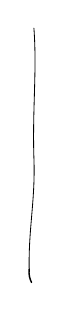
\begin{tikzpicture}[x=1cm,y=1cm,line cap=round]
\draw[line width=.30pt] (.04,0) .. controls (.08,-.55) and (.02,-1.02) .. (.04,-1.65)
 .. controls (.06,-2.18) and (-.03,-2.54) .. (-.02,-3.06);
\draw[line width=.52pt] (-.02,-3.06) .. controls (-.03,-3.13) and (-.01,-3.19) .. (.01,-3.23);
\end{tikzpicture}}}
\[
(38)\qquad \uline{g\rho(g)\rho^2(g)=1},
\]
where $g$ is given by (40), and where $u$ is expressed in terms of
\deleted{$g$} $g$ hence of $g_0,\gamma$ by
\[
(36)\qquad
\left\{\begin{aligned}
u(\sigma_\infty)&=\sigma_\infty\\
u(\rho)&=g\rho\qquad
\left(=\underbrace{\sigma_\infty(g_0)\ell_1^\gamma\rho(g_0)^{-1}}_g\rho\right).
\end{aligned}\right.
\]

\deleted{The relation (42)\inserted{\unsure{cf. = above}}, then reads,
since $L_0$ is generated by}
\[
\deleted{\ell_0=\underbrace{\ell'_0}_{\varepsilon_0}^{2}=(\sigma_\infty\rho)^2\deleted{\unsure{\sigma_\infty}}=\sigma_\infty\rho\sigma_\infty\rho}
\]
\[
\deleted{\underbrace{(u(\sigma_\infty\rho))}_{
\substack{\sigma_\infty g\rho=g_0\sigma_\infty \ell_1^\gamma\rho g_0^{-1}
=\operatorname{int}(g_0)(\sigma_\infty \ell_1^\gamma\rho)}}^{\unsure{2|4}}
\in\operatorname{int}(g_0)(\unsure{L'_0|L_0})\qquad\text{\unsure{now}}}
\]
\[
\deleted{\operatorname{int}(g_0)(\sigma_\infty \ell_1^\gamma\rho)^2\deleted{\unsure{g_0^{-1}}=1}}
\]
\deleted{thus (42) reads}
\[
\deleted{(\sigma_\infty \ell_1^\gamma\rho)^2\in L_0}
\]
\deleted{\unsure{i.e.}}
\[
\deleted{
\underbrace{\sigma_\infty \ell_1^\gamma\sigma_\infty}_{
    \underbrace{\sigma_\infty(\ell_1)}_{\ell_0}^{\gamma}}
  \underbrace{\sigma_\infty\illegible{1}\rho}_{\varepsilon_0}
}
\]
\margin{\deleted{N.B. $\operatorname{int}(g_0^{-1})u(\ell_0)$}}
\margin{\deleted{N.B. we have
$(\operatorname{int}(g_0^{-1})u)(\ell_0)
=(\sigma_\infty \ell_1^\gamma\rho)^2=\ell_0^{2\gamma+1}$}}
\deleted{\unsure{i.e.}}
\[
\deleted{\overset{\varepsilon_0^{2\gamma+1}}{\unsure{\ell_0^\gamma}\ \underbrace{\varepsilon_0}_{\unsure{\varepsilon_0^{2\gamma}}}}\in L_0}
\]
\deleted{therefore \unsure{\ldots}}
\[
\deleted{\unsure{\operatorname{int}(g_0)}\quad u(\ell_0)=}
\]

The relation (42), or the \unsure{apparently} stronger relation
\[
(43)\qquad u(L'_0)\subset\operatorname{int}(g_0)(L'_0)
\]
reads
\[
\underbrace{\operatorname{int}(g_0^{-1})\,
\underbrace{u(\underbrace{\sigma_\infty\rho}_{\ell'_0=\varepsilon_0})}_{
\sigma_\infty g\rho=g_0\sigma_\infty \ell_1^\gamma\rho g_0^{-1}}}_{
\sigma_\infty \ell_1^\gamma\rho
=\underbrace{\underbrace{\sigma_\infty \ell_1^\gamma\sigma_\infty}_{
 \underbrace{\sigma_\infty(\ell_1)^\gamma}_{\ell_0^\gamma=\varepsilon_0^{2\gamma}}}
\underbrace{\sigma_\infty\rho}_{\deleted{\unsure{\sigma_\infty\rho}}\varepsilon_0}}_{
\varepsilon_0^{2\gamma+1}}}
\in L'_0
\]
\margin{\uline{N.B.} we have
$\operatorname{int}(g_0^{-1})u(\underbrace{\ell'_0}_{\varepsilon_0})
=\varepsilon_0^{2\gamma+1}$}
\unsure{is satisfied} automatically, we \unsure{will have}
even
\[
\deleted{(44)\qquad u(\ell'_0)=u(\varepsilon_0)
=\operatorname{int}(g_0)(\ell'}
\]

\clearpage
\LMcote{140-3}
\typeout{LMLAYOUTSCAN 140-3 85}
\scanpage{85}

it is generated by complex conjugation $\tau$
\[
(5)\qquad ,\quad \tau(z)=\bar z,
\]
the five other elements of $\mathcal T_{0,3}$ are
\[
\deleted{\unsure{\tau\sigma}}\quad(6)\qquad
\tau\dot\sigma_0=\dot\tau_0,\quad
\tau\dot\sigma_1=\dot\tau_1,\quad
\tau\dot\sigma_\infty=\dot\tau_\infty,\quad
\tau\rho,\quad\tau\rho^{-1}=(\tau\rho)^{-1},
\]
the \unsure{anti-involutions|anti-involutions} $\tau'_i$ $(i=0,1,\infty)$ are particularly interesting, \unsure{given} by
\[
(7)\qquad
\unsure{\dot\tau'_0(z)}=\frac{\bar z}{\bar z-1},\quad
\unsure{\dot\tau'_1(z)}=\frac1{\bar z},\quad
\dot\tau'_\infty(z)=1-\bar z.
\]

The fixed points \deleted{\unsure{in $U_{0,3}$}} of the \inserted{\illegible{1}} conformal automorphisms of \deleted{\illegible{2}} $(\mathbb P^{1\mathrm{an}},\{0,1,\infty\})$ are the following
\[
\begin{gathered}
(8)\qquad
\left\{\begin{array}{l}
(\mathbb P^1_{\mathbb C})^{\dot\sigma_0}=\{0,2\},\\[3pt]
(\mathbb P^1_{\mathbb C})^{\dot\sigma_1}=\{1,-1\},\\[3pt]
(\mathbb P^1_{\mathbb C})^{\dot\sigma_\infty}=\{\infty,\frac12\}\\[3pt]
\mathbb P_{\mathbb C}^{1\,\dot\rho}=\mathbb P^{1\,\dot\rho^{-1}}=\{-\bar j,-j\}
\end{array}\right.\\[6pt]
\begin{array}{l}
\text{where }j=\exp 2i\pi/3=\dfrac{-1+i\sqrt3}{2}\quad\text{primitive root}\quad\text{$3^{\unsure{\mathrm{ième}|\mathrm{ème}}}$ of $1$}\\[5pt]
-\bar j=\exp 2i\pi/6=\dfrac{1+i\sqrt3}{2}\quad\text{primitive root}\quad\text{$6^{\unsure{\mathrm{ième}|\mathrm{ème}}}$ of $1$}
\end{array}\end{gathered}
\]

\margin{N.B. $\mathbb P_{\mathbb C}^{1\,\dot\rho\tau}=\mathbb P_{\mathbb C}^{1\,\dot\rho^{-1}\tau}=\varnothing$}

\[
(9)\qquad
\left\{\begin{array}{l}
\mathbb P_{\mathbb C}^{1\,\tau}=\mathbb P_{\mathbb R}^{1}\\[3pt]
\mathbb P_{\mathbb C}^{1\,\dot\tau'_0}=\{x+iy\mid(x-1)^2+y^2=1\}\\[-1pt]
\quad\inserted{=\{z\mid z+\bar z=z\bar z\}\unsure{=\frac1z|=\frac12}}
\inserted{\unsure{=\frac12-\mathbb U}},\\[3pt]
\mathbb P_{\mathbb C}^{1\,\dot\tau'_1}=\{z\mid z\bar z=1\}=\{x+iy\mid x^2+y^2=1\}=\mathbb U\\[3pt]
\mathbb P_{\mathbb C}^{1\,\dot\tau'_\infty}=\{z\mid z+\bar z=1\}=\{x+iy\mid x=\frac12\}=\frac12+i\mathbb R;
\end{array}\right.
\]

The most suggestive picture is probably that of the Riemann sphere, where $\tau,\dot\tau'_0,\dot\tau'_1,\dot\tau'_\infty$ appear as the \deleted{\unsure{symmetries}}\inserted{\uline{reflections}} with respect to the corresponding \deleted{``equators''}\inserted{``\unsure{gr\textsuperscript{eat}|great} circles''}, which for $\tau$ is ``the equator'' and for the others are the great circles \inserted{``meridians''}, passing through the poles $-\bar j,-j$, which effect the cutting up of the equator into six circular segments, by the subdivision points $0,\frac12,1,2,\infty,-1$.

\figure{\begin{tikzpicture}[x=.022cm,y=-.022cm,line cap=round,line join=round,font=\scriptsize]
\coordinate (N) at (110,8);
\coordinate (S) at (113,216);
\draw[line width=.4pt] (N) .. controls (62,1) and (11,43) .. (5,105)
 .. controls (-1,158) and (42,208) .. (S)
 .. controls (168,224) and (214,183) .. (220,114);
\draw[line width=.35pt] (N) .. controls (175,0) and (209,48) .. (224,101);
\begin{scope}
\clip (N) .. controls (62,47) and (32,109) .. (33,151)
 .. controls (60,160) and (91,164) .. (113,158)
 .. controls (114,100) and (112,43) .. (N);
\foreach \a in {-80,-58,-36,-14,8,30,52,74,96,118,140,162}
  \draw[line width=.3pt] (-15,\a)--(145,{\a+165});
\end{scope}
\draw[dash pattern=on 3pt off 2pt,line width=.45pt] (N)
 .. controls (58,40) and (26,93) .. (33,151)
 .. controls (38,187) and (77,213) .. (S);
\draw[dash pattern=on 3pt off 2pt,line width=.45pt] (N)
 .. controls (101,51) and (99,95) .. (99,145)
 .. controls (96,180) and (106,206) .. (S);
\draw[dash pattern=on 3pt off 2pt,line width=.45pt] (N)
 .. controls (125,41) and (121,113) .. (113,158)
 .. controls (111,183) and (113,205) .. (S);
\draw[dash pattern=on 3pt off 2pt,line width=.45pt] (N)
 .. controls (167,25) and (177,80) .. (180,144)
 .. controls (179,182) and (153,213) .. (S);
\draw[dash pattern=on 3pt off 2pt,line width=.35pt] (N)
 .. controls (53,15) and (10,62) .. (5,105)
 .. controls (8,161) and (47,207) .. (S);
\draw[dash pattern=on 3pt off 2pt,line width=.4pt] (5,109)
 .. controls (46,96) and (92,91) .. (103,96)
 .. controls (150,91) and (193,91) .. (218,108);
\draw[line width=.4pt] (5,109) .. controls (-2,133) and (13,144) .. (33,151)
 .. controls (80,171) and (148,155) .. (180,146)
 .. controls (204,142) and (224,134) .. (220,114);
\draw[->,line width=.7pt] (98,96)--(86,98);
\draw[->,line width=.6pt] (109,18) .. controls (123,28) and (119,45) .. (115,58);
\draw[->,line width=.6pt] (97,180)--(98,164);
\draw[->,line width=.6pt] (174,157)--(181,144);
\draw[line width=.65pt] (27,141)--(32,151)--(37,143);
\draw[line width=.65pt] (62,158)--(71,159)--(66,154);
\foreach \p in {(110,8),(113,216),(103,96),(33,151),(113,158),(180,146)}
  \fill \p circle[radius=2.4];
\foreach \p in {(5,109),(180,94)}
  \fill \p circle[radius=1.1];
\node[inner sep=0pt] at (111,-9) {$-\bar j$};
\node[inner sep=0pt] at (115,235) {$-j$};
\node[inner sep=0pt] at (5,96) {$-1$};
\node[inner sep=0pt] at (87,90) {$\infty$};
\node[inner sep=0pt] at (187,92) {$2$};
\node[inner sep=0pt] at (30,166) {$0$};
\node[inner sep=0pt] at (123,173) {$\frac12$};
\node[inner sep=0pt] at (185,159) {$1$};
\node[inner sep=0pt,rotate=16] at (60,66) {$\dot\tau'_0=\dot r_1$};
\node[inner sep=0pt] at (137,79) {$\dot\tau'_\infty$};
\node[inner sep=0pt,rotate=-68] at (137,107) {$=\dot r_0$};
\node[inner sep=0pt,rotate=-12] at (76,176) {$\unsure{\dot\tau}=\unsure{\dot r}_\infty$};
\end{tikzpicture}}

Let us also note the formulas
\[
(10)\qquad
\left\{\begin{array}{l}
\dot\rho\dot\tau'_0\dot\rho^{-1}=\dot\tau'_1,\quad
\dot\rho\dot\tau'_1\dot\rho^{-1}=\dot\tau'_\infty,\quad
\dot\rho\dot\tau'_\infty\dot\rho^{-1}=\dot\tau'_0\\[3pt]
\dot\tau'_0\dot\tau'_1=\dot\tau'_1\dot\tau'_\infty=\dot\tau'_\infty\dot\tau'_0=\dot\rho
\end{array}\right.
\]
\margin{84}

\clearpage
\LMcote{140-3}
\typeout{LMLAYOUTSCAN 140-3 88}
\scanpage{88}
\mspage{333}

We have
\[
\tag{22}
\left\{\begin{aligned}
(\sigma_\infty\rho)^2&=(\rho\sigma_1)^2=\ell_0=\varepsilon_0^2,&
\varepsilon_0&\overset{\unsure{\text{definition}|\text{definition}}}{=}\sigma_\infty\rho=\rho\sigma_1\deleted{\unsure{\overset{\mathrm{dfn}}{=}}}
\\[-1pt]&&&\quad(\mathrm{NB}\ \sigma_\infty=\rho\sigma_1\rho^{-1})\\
(\sigma_0\rho)^2&=(\rho\sigma_\infty)^2=\ell_1=\varepsilon_1^2,&
\varepsilon_1&=\unsure{\sigma_0}\rho=\rho\sigma_\infty\\
(\sigma_1\rho)^2&=(\rho\unsure{\sigma_\infty|\sigma_0})^2=\ell_\infty=\varepsilon_\infty^2,&
\varepsilon_\infty&=\sigma_1\rho=\rho\sigma_0
\end{aligned}\right.
\]

The element $\varepsilon_i\in\mathfrak S_{0,3}$
(in fact $\varepsilon_i\in\mathfrak S_{0,3}^{+}$) is over $\dot\sigma_i$,
it is \uline{characterized} by the condition
\[
\varepsilon_i^2=\ell_i.
\]

In the group $\mathcal T_{0,3}$ of order $12$, there are seven \unsure{involutive} elements
$\dot\sigma_0,\dot\sigma_1,\dot\sigma_\infty,\tau,\dot\tau'_0,\dot\tau'_1,\dot\tau'_\infty$,
\deleted{and \unsure{four}} \inserted{two} elements of order $3$
$\dot\rho,\dot\rho^{-1}$, \inserted{and \uline{two of order $6$}}
$\dot\rho\tau,\dot\rho^{-1}\tau$ (in addition to the identity).

\inserted{Except for the last two (for which this is not possible$^*$)}
We \unsure{have} \unsure{lifted} each of these elements to elements of the same order in
$\mathfrak S_{0,3}$.
\margin{$^*$ indeed ${\mathbb P^1}^{\dot\rho\tau}={\mathbb P^1}^{\dot\rho^{-1}\tau}=\varnothing$}
We know that the possibilities, mod $\Pi_{0,3}$-conjugation, \unsure{of|of the} such liftings,
correspond to the connected components of the fixed points \unsure{in|of} $U=U_{0,3}^{\mathrm{an}}$
of the corresponding \unsure{topological} automorphisms. --- for
$\dot\sigma_0,\dot\sigma_1,\dot\sigma_\infty,\dot\tau'_0,\dot\tau'_1,\dot\tau'_\infty$
there is only one possibility mod conjugation (we have chosen
$\sigma_0,\sigma_1,\sigma_\infty,\tau_0,\tau_1,\tau_\infty$
in the way that seemed most convenient for the calculations),
for $\tau$ there are three --- these are the three choices $\tau_0,\tau_1,\tau_\infty$
--- for $\dot\rho,\dot\rho^{-1}$ there are two,
\unsure{corresponding|corresponding} to the two poles $-\bar j,-j$ --- we have chosen the one that
corresponds to the pole $-\bar j$.
The liftings corresponding to $-j$ \unsure{can} be deduced from them by \unsure{conjugating} by a $\tau_i$:

\margin{87}

\clearpage
\LMcote{140-3}
\typeout{LMLAYOUTSCAN 140-3 107}
\scanpage{107}

\[
(81)\quad
\left\{\begin{aligned}
P&=(a+b)(c+d-b)&Q&=-a(c-b)-bc\overset{\inserted{\deleted{\text{if }\det g=+1}}}{=}\deleted{\unsure{1}}\delta-a(c+d-b)\\
R&=(c+d)^2-d(a+b)&S&=ad-c(c+d)=\underset{\inserted{\text{if }\det g=1}}{\delta}-c(c+d-b)\\
&\underset{\inserted{\text{if }\det g=+1}}{=}(c+d)(c+d-b)-\delta
\end{aligned}\right.
\]
where we have set $\delta=ad-bc=\det g$.

Comparing (81) and the expression (77) for $\rho^2(g^{-1})$, equation (79) -- which is also written
\[
g\rho(g)=\pm\rho^2(g^{-1})
\]
gives the following solutions.

\margin{Up to replacing $g$ by $\unsure{-g}$, \deleted{\illegible{5}} \unsure{we are reduced} to \unsure{determining} the solutions of the equation}

\[
(82)\qquad \unsure{g|\rho}\rho(g)\rho^2(g)=\unsure{+|\pm}1\qquad\text{i.e.}\quad \unsure{g|\rho}\rho(g)=\unsure{+|\pm}\rho^{-1}(g^{-1})\qquad\text{\uline{in $\mathrm{Gl}(2,\widehat{\mathbb Z})$}}
\]
\deleted{$\unsure{(82)}$ \illegible{2} $\unsure{g\rho(g)=+\rho^{-1}(g^{-1})}$.}
We distinguish the solutions according to the factors of the product
\[
\mathrm{Sl}(2,\widehat{\mathbb Z})'\simeq\prod_{\ell\ \mathrm{premier}}\mathrm{Sl}(2,\mathbb Z_\ell)'.
\]
\margin{\uline{N.B.} \unsure{We} \unsure{shall use|use} this study of equation (82) only in the case $\det g=1$, i.e. $\delta=1$, \unsure{unless I am mistaken}}

The relation
\[
\frac1\delta(a+b)=P=(a+b)(c+d-b)\qquad\text{in }\mathbb Z_\ell
\]
gives the two solutions $a+b=0$ or $c+d-b=1$ (since $\mathbb Z_\ell$ is an integral domain).

\deleted{1°) $(a+b)\ne0$ (in $\mathbb Z_\ell$) whence $c+d-b=1$
\[
(83)\qquad\boxed{c+d-b=\frac1\delta}.
\]
Given (83), we verify \unsure{at once} that the formulas \inserted{$g\rho(g)=\rho^{-1}(g^{-1})$} -- which remain to be checked
\[
\begin{aligned}
P&=(a+b)/\delta&Q&=(1-a)/\delta\\
R&=b/\delta&S&=(1-c)/\delta
\end{aligned}
\]
\inserted{\deleted{\illegible{1}} $\unsure{R=}$
\[
\begin{aligned}
Q&=\frac{c+d-\unsure{a}-b}{\delta}\left(=\unsure{\frac1{\delta^2}|\frac1\delta}-\frac a\delta\right),\\
R&=\frac b\delta,\quad S=\frac{d-b}{\delta}\left(=\frac1{\delta^2}-\frac c\delta\right)
\end{aligned}
\]}
(84) are equivalent to \illegible{5} (82) \illegible{1}
\[
(84)\qquad\boxed{\delta^3=1}.
\]
}

\margin{The necessity of this formula (84) was obvious a priori.}

\deleted{2°) $a+b=0$ i.e. $a=-b$, i.e. $g=\begin{pmatrix}-b&b\\c&d\end{pmatrix}$, and
\[
-b(c+d)=1
\]
\[
(84)\quad\left\{\begin{aligned}
\det g&=-b(c+d)=\delta\quad(\text{thus }\delta+b(c+d)=0;\unsure{)}\\[-1pt]&\quad d=-\frac\delta b-c\\
P&=0,\\ Q&=\delta+b(c+d-b)=-b^2\\
R&=(c+d)^2=\frac{\delta^2}{b^2},\\ S&=\unsure{ad}\ \illegible{1}\\[-1pt]&{-c(c+d)+ad=1-c(\unsure{c+d-b})}\\
&\deleted{\illegible{1}c}=\delta+c\left(\frac\delta b+b\right)
\end{aligned}\right.
\]
}

\clearpage
\LMcote{140-3}
\typeout{LMLAYOUTSCAN 140-3 320}
\scanpage{320}
\mspage{460}

of $\alpha$ as above, hence $\mu=\det\underline u$, hence
and it \deleted{suffices} \deleted{$\varepsilon\beta\sigma(\beta)^{-1}=\unsure{\alpha|\eta}$}
remains to determine $\beta$ as
$\beta=\underline u\underline b^{-1}$, with $\underline b\in\Gamma N'_\sigma$
arbitrary, $\varepsilon$ being defined then in terms of the choice of $\underline b$
as being $\varepsilon_\sigma(\underline b)$. The condition for
fixed $\unsure{\alpha_0|\alpha}$ to be completable by $(\beta,\mu,\varepsilon)$
to $(\alpha,\beta,\mu,\varepsilon)\in\Gamma\mathcal G^{\unsure{\alpha|*}}_{\rho,\sigma}$,
is always the condition that the coefficient $D$ \deleted{of $\zeta=\alpha\unsure{+}$}
\[
\tag{33}
\zeta=\alpha\rho(\alpha)^{-1}=\begin{pmatrix}A&B\\C&D\end{pmatrix}
\]
be invertible, which \inserted{makes it possible to} \unsure{will determine|determine} $\mu$ by
\[
\tag{34}
\mu=1/D.
\]

Let us put
\[
\tag{35}
\alpha=\begin{pmatrix}a&b\\c&d\end{pmatrix}
\]
and make $\alpha\rho(\alpha)^{-1}$ explicit; with
$\rho=\begin{pmatrix}0&1\\v&1\end{pmatrix}$

\margin{$\delta=\det\alpha=ad-bc$}
\[
\begin{aligned}
\alpha\rho(\alpha)^{-1}
&=\begin{pmatrix}a&b\\c&d\end{pmatrix}
\begin{pmatrix}0&1\\v&\deleted{\unsure{w}}\inserted{1}\end{pmatrix}
\frac1\delta\begin{pmatrix}d&-b\\-c&a\end{pmatrix}
\left(-\frac1v\right)
\begin{pmatrix}\deleted{\unsure{w}}\inserted{1}&-1\\-v&0\end{pmatrix}\\
&=-\frac1{\unsure{\delta}v}
\begin{pmatrix}bv&a+b\deleted{\unsure{w}}\\dv&c+d\deleted{\unsure{w}}\end{pmatrix}
\begin{pmatrix}d\deleted{\unsure{w}}+bv&-d\\-c\deleted{\unsure{w}}-av&c\end{pmatrix},
\end{aligned}
\]
hence
\[
\deleted{\unsure{=\frac1{\delta v}}}
\]
\[
\tag{36}
\left\{\begin{aligned}
(-\delta v)A&=\unsure{v}b(d+\unsure{vb|bv})\unsure{-}(a+b)(c+va)
&(-\delta v)B&=-vbd+c(a+b)\\
(-\delta v)C&=vd(d+vb)-(c+d)(c+va)
&(-\delta v)D&=-vd^2+cd+c^2,
\end{aligned}\right.
\]
the most essential quantity thus being
\[
\tag{37}
\left\{\begin{aligned}
(-\unsure{\delta}v)D&=-vd^2+cd+c^2=\det(d\rho+c),\\
\text{\deleted{\unsure{and after that|and after calculation}} where }&\\[3pt]
&\left\{\begin{aligned}
\deleted{\unsure{\alpha}}\ \delta&=\det\alpha=ad-bc,\\
v&\ \text{the \unsure{parameter|coefficient} which defines }\\&\rho=\begin{pmatrix}0&1\\v&1\end{pmatrix}
\end{aligned}\right.
\end{aligned}\right.
\]

\clearpage
\LMcote{140-3}
\typeout{LMLAYOUTSCAN 140-3 328}
\scanpage{328}

so the condition reads $\unsure{v|\nu}=-1$, i.e. this is condition $3^\circ$, but then the expression (23) for $\rho^3$ shows us that $\rho^3=-1$.

\uline{\unsure{Remarks|Remark}} The preceding conditions imply the formulas
\[
\begin{aligned}
(24)\qquad &\varepsilon_0=\sigma\rho\\
(25)\qquad &\varepsilon_1=\rho\sigma\\
(26)\qquad &\rho\varepsilon_1=\varepsilon_0^{-1}\\
(27)\qquad &\rho^2\sigma=\varepsilon_0^{-1}
\end{aligned}
\]
each of which \inserted{except the last (27)} implies them in turn
--- for example we have $\varepsilon_0=-\sigma^{-1}\rho$ \inserted{(7)}, so (24) is equivalent to \inserted{$\sigma=-\sigma^{-1}$ i.e.} $\sigma^2=-1$, and (25) is equivalent to (24) by applying $\operatorname{int}(\rho)$ to both \unsure{sides}.

We have moreover
\[
\rho\varepsilon_1=
\begin{pmatrix}0&1\\\unsure{v|\nu}&\unsure{w|\omega}\end{pmatrix}
\begin{pmatrix}1&0\\1&1\end{pmatrix}
=\begin{pmatrix}1&1\\\unsure{v|\nu}+\unsure{w|\omega}&\unsure{\unsure{w|\omega}^{\prime}|\unsure{w|\omega}}\end{pmatrix},
\qquad
\varepsilon_0^{-1}=\begin{pmatrix}1&1\\0&1\end{pmatrix}
\]
which shows that $\rho\varepsilon_1=\varepsilon_0^{-1}$ is equivalent to:
\[
\unsure{w|\omega}=1,\quad \unsure{v|\nu}+\unsure{w|\omega}=0\qquad\text{i.e.}\quad \unsure{w|\omega}=1,\unsure{v|\nu}=-1\quad\text{i.e.}\quad
\rho=\begin{pmatrix}0&1\\-1&1\end{pmatrix},
\]
OK. Composing (25) \inserted{(in the form $\rho\varepsilon_1=\rho^2\sigma$)} and (26) we find (27) as a consequence of the conditions $2^\circ)+3^\circ)$; \deleted{\unsure{the}}\inserted{Let us try to prove} converse implication \deleted{\unsure{follows}}\inserted{by} \deleted{from} a brute-force calculation
\[\begin{gathered}\deleted{\rho^2\sigma=}\rho^2\sigma=
\begin{pmatrix}
-\unsure{v|\nu}\unsure{w|\omega}&\unsure{w|\omega}-(\unsure{v|\nu}+\unsure{w|\omega}^2)\\
-\unsure{v|\nu}(\unsure{v|\nu}+\unsure{w|\omega}^2)&\unsure{\begin{gathered}-\unsure{w|\omega}(\unsure{w|\omega}^2+2\unsure{v|\nu})+\unsure{v|\nu}-\unsure{w|\omega}^2\\[-1pt]|-\unsure{w|\omega}(\unsure{w|\omega}^2+2\unsure{v|\nu})+\unsure{v|\nu}+\unsure{w|\omega}^2\end{gathered}}
\end{pmatrix},\\[5pt]
\varepsilon_0^{-1}=\begin{pmatrix}1&\unsure{-1/\unsure{v|\nu}}\\0&1\end{pmatrix}
\end{gathered}\]
\deleted{since $\unsure{v|\nu}$ invertible} we can have the equality $\rho^2\sigma=\unsure{-\varepsilon_0^{-1}|\varepsilon_0^{-1}}$ only if $-\unsure{v|\nu}(\unsure{v|\nu}+\unsure{w|\omega}^2)=0$, \unsure{this implies|which implies} ($\unsure{v|\nu}$ invertible!) $\unsure{v|\nu}+\unsure{w|\omega}^2=0$, \deleted{\unsure{whence}}\inserted{i.e. $\unsure{v|\nu}=-\unsure{w|\omega}^2$},

\mspage{327}

\clearpage
\LMcote{140-3}
\typeout{LMLAYOUTSCAN 140-3 329}
\scanpage{329}
\mspage{465}

\[
\rho^2\sigma=\begin{pmatrix}\unsure{w|\omega}^3&\unsure{w|\omega}\\0&\deleted{\unsure{-w(1+2w)}}\inserted{\unsure{w|\omega}^3}\end{pmatrix},
\]
This shows that
\deleted{$\rho^2\sigma=\varepsilon_0^{-1}$ \unsure{iff} $\unsure{w|\omega}=1$ OK.}
\margin{\deleted{\unsure{We have in addition to} \illegible{4}}
\unsure{$\unsure{v|\nu}=-\unsure{w|\omega}^2$} \deleted{\illegible{2}}
\unsure{i.e. $\unsure{v|\nu}=-1,\unsure{w|\omega}=1$}}
\inserted{
\[
\begin{gathered}(27\mathrm{bis})\qquad
\rho^2\sigma=\varepsilon_0^{-1}\Longleftrightarrow
\left\{\unsure{v|\nu}+\unsure{w|\omega}^2=0,\ \unsure{w|\omega}^3=1\right.
\\[4pt]
\left(\Rightarrow \unsure{v|\nu}=-\unsure{w|\omega}^2=-1/\unsure{w|\omega}\ \text{i.e.}\ \unsure{w|\omega}=-1/\unsure{v|\nu},\ \mathrm{OK}\right)
\end{gathered}\]
}

But (27), on multiplying by $\rho$, is also equivalent to
\[\deleted{\unsure{(27)}\,\illegible{1}}\rho^3\sigma=\deleted{\unsure{u}}\rho\varepsilon_0^{-1}
\]
now we know that $\varepsilon_0=\unsure{-\sigma^{-1}\rho}$ \inserted{(7)} i.e. $\varepsilon_0^{-1}=-\deleted{\unsure{\sigma}}\rho^{-1}\unsure{\sigma|\sigma_0}$
i.e. $\rho\varepsilon_0^{-1}=-\sigma$, so the preceding relation also reads $\rho^3\sigma=-\sigma$ or again
\[
(28)\qquad \boxed{\rho^3=-1}.
\]
We can see \deleted{\unsure{this}} the equivalence \deleted{directly}\inserted{of (28) with the conditions (27bis)} by computing $\rho^3$ in terms of $\unsure{v|\nu},\unsure{w|\omega}$, we find
\[
(29)\qquad
\rho^3=\begin{pmatrix}\unsure{v|\nu}\unsure{w|\omega}&\unsure{v|\nu}+\unsure{w|\omega}^2\\\unsure{v|\nu}(\unsure{v|\nu}+\unsure{w|\omega}^2)&\unsure{w|\omega}(2\unsure{v|\nu}+\unsure{w|\omega}^2)\end{pmatrix}
\]
And we can have $\widetilde\rho^3=1$ i.e. $\rho^3$ a scalar only if \deleted{$\unsure{v|\nu}+\unsure{w|\omega}^2=$}
\[
\unsure{v|\nu}+\unsure{w|\omega}^2=0\qquad\text{i.e.}\quad \unsure{v|\nu}=-\unsure{w|\omega}^2
\]
which implies
\[
\rho^3=\begin{pmatrix}-\unsure{w|\omega}^3&0\\0&-\unsure{w|\omega}^3\end{pmatrix}
\]
i.e. we find

\uline{Lemma} We have $\widetilde\rho^3=1$ iff $\unsure{v|\nu}+\unsure{w|\omega}^2=0$ i.e. $\unsure{v|\nu}=-\unsure{w|\omega}^2$ i.e. we have
\[
(30)\qquad
\rho=\begin{pmatrix}0&1\\-\unsure{w|\omega}^2&\unsure{w|\omega}\end{pmatrix},
\]
and then we have
\[
(31)\qquad \rho^3=\unsure{-}\unsure{w|\omega}^3\cdot1\ ,
\]
so we have
\[
(32)\qquad
\rho^3=-1\Longleftrightarrow
\deleted{\unsure{\unsure{v|\nu}=-\unsure{w|\omega}^2}}\quad
\begin{gathered}
\unsure{w|\omega}^3=1\ \text{i.e. }\unsure{w|\omega}\in\Gamma\mu_3\\
\inserted{\uline{and}\quad \unsure{v|\nu}=-\unsure{w|\omega}^2\ (= -1/\unsure{w|\omega})}
\end{gathered}
\]

\mspage{328}

\clearpage
\LMcote{140-3}
\typeout{LMLAYOUTSCAN 140-3 413}
\scanpage{413}
\mspage{508}

\uline{$\overline{\mathrm{XI}}$}\quad\uline{Recapitulation on the group} $\mathcal{M}_{\rho,\sigma}$.

\margin{\uline{Preliminaries}}

\textcircled{$1^\circ$} Given, over a scheme $S$, a form $G$ of $\mathrm{Gl}(2)$, hence forms $SG$, $PG$ of $\mathrm{Sl}(2)$, $\unsure{\mathrm{GP}(1)|\mathrm{PGl}(1)}$, and two sections $\widetilde\rho,\widetilde\sigma$ of $PG$, and a \unsure{1-parameter} \deleted{\unsure{unipotent|multiplicative}} additive \unsure{bordered|based} subgroup
\diagram{\begin{tikzcd}[ampersand replacement=\&,column sep=large]
\widetilde{\uline{\varepsilon}}_0:\ G_a \arrow[r,hook] \& PG
\end{tikzcd}}
\inserted{$\unsure{\varepsilon_0|G_a}$}
(which amounts to the same thing, a \deleted{\unsure{of}} regular unipotent section \unsure{of} $\varepsilon_0$ of $G$, or a regular nilpotent section $N_0$ in the form $\mathcal M$ of $\mathrm{M}_2(\mathcal O_S)$ associated to $G$) --- satisfying the conditions
\[
\begin{aligned}
(1)\quad &\widetilde\sigma^{-1}\widetilde\rho
  =\widetilde{\uline{\varepsilon}}_0(1),\qquad
  \widetilde{\uline{\varepsilon}}_0\text{ and }
  \widetilde{\uline{\varepsilon}}_1
  =\rho\bigl(\widetilde{\uline{\varepsilon}}_0\bigr)
  \bigl(=\sigma\bigl(\widetilde{\uline{\varepsilon}}_0\bigr)\bigr)
  \text{ are}\\
 &\hspace{10em}\text{independent on each fiber}\\[4pt]
(2)\quad &\mathrm{Tr}\,\sigma=0\qquad
 \text{if }\sigma\text{ is a local lifting of }\widetilde\sigma,
\end{aligned}
\]

We define \uline{canonical} liftings $\rho$, $\sigma$ of $\widetilde\rho,\widetilde\sigma$ to $G$, \deleted{\unsure{satisfy}} by the conditions
\[
(3)\quad\deleted{\unsure{\sigma\rho}}
\left\{\begin{array}{ll}
 \varepsilon_0=-\sigma^{-1}\rho
 &\text{i.e. }\varepsilon_1=-\rho\sigma^{-1}\\
 \mathrm{Tr}(\rho+\sigma)=1
 &\text{i.e. }\mathrm{Tr}\,\rho=1,
\end{array}\right.
\]
and the constructions which follow make sense.

We construct a \unsure{pinning}
\diagram{\begin{tikzcd}[ampersand replacement=\&,column sep=large]
\deleted{(\unsure{4})}\ (5)\quad\deleted{\unsure{\tau_{\rho,\sigma}}=}\ \mathrm{Gl}(2)
 \arrow[r,"\sim"] \& G
\end{tikzcd}}
by the condition that $\varepsilon_1$ take the form
\[
(6)\qquad\varepsilon_1
 =\begin{pmatrix}1&0\\1&1\end{pmatrix}
\]
whence
\[
(7)\quad\left\{\begin{array}{l}
\displaystyle\rho=\begin{pmatrix}0&1\\\unsure{v|\upsilon}&1\end{pmatrix},\qquad
 \sigma=\begin{pmatrix}0&-1\\-\unsure{v|\upsilon}&0\end{pmatrix}
 \qquad(\unsure{v|\upsilon}\in\Gamma G_m\\[6pt]
\det\rho=\det\sigma=-\unsure{v|\upsilon}
\end{array}\right.
\]
\[
(8)\qquad\varepsilon_0
 =\begin{pmatrix}1&1/\unsure{v|\upsilon}\\0&1\end{pmatrix},
\]

\margin{412}

\clearpage
\LMcote{140-3}
\typeout{LMLAYOUTSCAN 140-3 425}
\scanpage{425}
\mspage{514}

\[
\tag{71}
\mathcal R_{\rho,\sigma}^{\circ}\simeq
\left\{\left(
 j_{T_0}(\mu^2),
 \underset{\substack{\rotatebox{90}{$\in$}\\ \Gamma T_\rho}}{\underline a},
 \underset{\substack{\rotatebox{90}{$\in$}\\ \Gamma T_\sigma}}{\underline b}
 \right)\cdot
 \underbrace{\mu j_G(\mu^{-2})}_{\inserted{\begin{gathered}
 \text{N.B. the}\\[-2pt]
 \text{determinant is }1\\[-2pt]
 \text{since }\det j_G(\mu^{-2})=\mu^{-2}
 \end{gathered}}}
 \;\middle|\;
 \begin{gathered}
 \unsure{\mu}\in\Gamma \mathbb G_m,\\[-2pt]
 \det\underline a=\det\underline b\deleted{\unsure{=\lambda^2}}\\[-2pt]
 \underline a\in\Gamma T_\rho,\qquad=\mu^2\\[-2pt]
 \underline b\in\Gamma T_\sigma,
 \end{gathered}\right\}
\]

where \inserted{$\unsure{j^{+}|j_G}$}
\[
\tag{72}
\left\{\begin{aligned}
 j(\unsure{\mu})&=\begin{pmatrix}\mu&1\\0&1\end{pmatrix}
 \in\Gamma SG\qquad(\mu\in\Gamma \mathbb G_m)\\
 j_{T_0}\deleted{(\unsure{\mu})}&:\mathbb G_m\longrightarrow T_0
 \quad\text{given by }j\\
 j_G&:\mathbb G_m\longrightarrow\unsure{\deleted{S}}G
 \quad\text{given by }j\text{ above.}
\end{aligned}\right.
\]

We thus find that the composite
\[
\tag{73}
\left\{\begin{gathered}
\diagram{\begin{tikzcd}[ampersand replacement=\&,column sep=large]
\mathcal R_{\rho,\sigma}^{\circ}
 \arrow[r,hook,"{\text{inclusion}}"'] \&
\mathcal M_{\rho,\sigma}^{\circ}
 \arrow[r,"{\text{canonical}}"'] \&
\begin{gathered}
\mathcal T_{\rho,\sigma}^{\circ}\simeq T_\rho\mathbin{\times}_{\mathbb G_m}T_\sigma\\
\shortparallel\\[-3pt]
\mathcal M_{\rho,\sigma}^{\circ}/\widetilde{\mathcal G}_{\rho,\sigma}^{+}
\end{gathered}
\end{tikzcd}}\\
\text{makes }\mathcal R_{\rho,\sigma}^{\circ}
 \text{ an \unsure{algebraic} covering}\\
\text{of }\mathcal T_{\rho,\sigma}^{\circ}
\end{gathered}\right.
\]

and more precisely that we have a cartesian diagram
\[
\tag{74}
\diagram{\begin{tikzcd}[ampersand replacement=\&,column sep=huge,row sep=large]
\mathcal R_{\rho,\sigma}^{\circ}
 \arrow[r,"{(73)}"]
 \arrow[d,"{\substack{\text{the canonical homomorphism}\\\text{of }(70)}}"']
 \arrow[dr,phantom,"{\text{cartesian}}",description] \&
T_\rho\mathbin{\times}_{\mathbb G_m}T_\sigma\simeq\mathcal T_{\rho,\sigma}^{\circ}
 \arrow[d,"{\text{canonical}}"]\\
\mathbb G_m \arrow[r,"{\mu\longmapsto\mu^2}"'] \&\mathbb G_m
\end{tikzcd}}
\]

\noindent(75)\quad\uline{Proposition} :
$\mathcal R_{\rho,\sigma}^{\circ}=\uline{Centr}(\mathcal M_{\rho,\sigma}^{\circ})$

Obviously the center of $\mathcal M_{\rho,\sigma}^{\circ}$ is contained
 in $\mathcal R_{\rho,\sigma}^{\circ}$, precisely the inverse image of the center

\par\noindent 424

\clearpage
\LMcote{140-3}
\typeout{LMLAYOUTSCAN 140-3 446}
\scanpage{446}

\deleted{$\uline{\mathcal O}_S$. Let us denote by \deleted{$\unsure{\mu'_2}$}
\[
\tag{131}
\begin{gathered}
\mu'_2\subset ST_\sigma\\[-.5em]
\rotatebox{90}{$=$}\\[-.5em]
\deleted{\unsure{\uline{\mathrm{Cent}}}}(ST_\sigma)^{\mu_2}
\end{gathered}
\]
\unsure{this|a} subgroup of}

whence \unsure{finally|finally}, \unsure{namely|i.e.}:
\[
\tag{128}
\underset{\unsure{=}}{\uline{\mathrm{Cent}}(\mathcal M_{\rho,\sigma})}
\simeq S'T_\rho\times\mu_2\times G_m
\subset R_{\rho,\sigma}\simeq S'T_\rho\times SN'_\sigma\times G_m
\]
whence
\[
\tag{129}
\uline{\mathrm{Cent}}(\mathcal M_{\rho,\sigma})\cap\mathcal M_{\rho,\sigma}^{\circ}
=ST_\rho\times\mu_2\times G_m
\subset R_{\rho,\sigma}^{\circ}\simeq ST_\rho\times ST_\sigma\times G_m
\]

Let us return to the integral sections in the absolute modular case
\[
\tag{130}
R_{\rho,\sigma}(\mathbb Z)\simeq
\underbrace{S'T_\rho(\mathbb Z)}_{\unsure{T_\rho}(\mathbb Z)\simeq\mathbb Z/6\mathbb Z}
\times
\underbrace{SN'_\sigma(\mathbb Z)}_{T_\sigma(\mathbb Z)=\mathbb Z/4\mathbb Z}
\times
\underbrace{G_m(\mathbb Z)}_{\mu_2(\mathbb Z)\simeq\pm1}
\]
\[
\tag{131}
\begin{aligned}
\uline{\mathrm{Cent}}(\mathcal M_{\rho,\sigma})\unsure{[\mathbb Z]|(\mathbb Z)}
&\simeq S'(T_\rho\unsure{[\mathbb Z]|(\mathbb Z)})\times\mu_2(\mathbb Z)\times G_m(\mathbb Z)\\
&\simeq\mathbb Z/6\mathbb Z\times\{\pm1\}\times\{\pm1\}
\end{aligned}
\]
and for the record (cf. (75), p. 514)
\[
\tag{132}
\begin{aligned}
\underbrace{\uline{\mathrm{Cent}}(\mathcal M_{\rho,\sigma}^{\circ})}_{\substack{R_{\rho,\sigma}^{\circ}\\\simeq ST_\rho\times ST_\sigma\times G_m}}(\mathbb Z)
&\simeq ST_\rho(\mathbb Z)\times ST_\sigma(\mathbb Z)\times G_m(\mathbb Z)\\
&\simeq\mathbb Z/6\mathbb Z\times\mathbb Z/4\mathbb Z\times\{\pm1\}.
\end{aligned}
\]

In summary, we have the diagram of \inserted{strict} inclusions of group schemes
\[
\tag{133}
\diagram{\begin{tikzcd}[ampersand replacement=\&,column sep=1.5em,row sep=5em,column sep=9pt,row sep=14pt,execute at begin picture={\fontsize{10}{12}\selectfont}]
\text{dimension }3 \&
\begin{gathered}
\uline{\mathrm{Cent}}(\mathcal M_{\rho,\sigma}^{\circ})=R_{\rho,\sigma}^{\circ}\\
\simeq ST_\rho\times ST_\sigma\times G_m
\end{gathered}
\arrow[rr,hook,"{{{\substack{\text{(quotient}\\\mu_2\times\mu_2\text{)}}}}}"']
\& \&
\begin{gathered}
R_{\rho,\sigma}\\
\simeq S'T_\rho\times SN'_\sigma\times G_m
\end{gathered}
\&\text{dimension }3\\
\text{dimension }2\&
\begin{gathered}
\uline{\mathrm{Cent}}(\mathcal M_{\rho,\sigma})\cap\mathcal M_{\rho,\sigma}^{\circ}\\
=ST_\rho\times\mu_2\times G_m
\end{gathered}
\arrow[u,hook]\arrow[rr,hook,"{{{\substack{\text{(quotient}\\\mu_2\text{)}}}}}"']
\&\&
\begin{gathered}
\uline{\mathrm{Cent}}(\mathcal M_{\rho,\sigma})\\
\simeq S'T_\rho\times\deleted{\unsure{SN'_\sigma}}\inserted{\unsure{\mu_2}}\times G_m)
\end{gathered}
\arrow[u,hook]
\&\text{dimension }2
\end{tikzcd}}
\]

\mspage{445}

\begin{center}
{\small
445\\
\texttt{https://grothendieck.umontpellier.fr}\\
Université de Montpellier, UMR CNRS 5149, Case courrier 051, Place Eugène Bataillon\\
34095 Montpellier cedex 5 - France
}
\end{center}

\clearpage
\LMcote{140-3}
\typeout{LMLAYOUTSCAN 140-3 448}
\scanpage{448}

\margin{\uline{\unsure{Where we define}}\quad\uline{$\mathcal{M}_{\rho,\sigma}$}}

\textcircled{$7^\circ$}\quad Let us make a \unsure{list|little} \unsure{recapitulation|recapitulatory} of the main group homomorphisms considered in the course of section $6^\circ$, involving the group $\mathcal{M}_{\rho,\sigma}$
\[
(134)\qquad
\diagram{\begin{tikzcd}[ampersand replacement=\&,row sep=small,column sep=large]
 \& SG\arrow[dddr,"{j_G}"] \& \& G\arrow[r]\arrow[dr,"{\delta_G=\det_G}"] \& PG\\
 \& \& \& \& G_m\\
 \& S'T_\rho\arrow[dr,"{j_\rho}"] \& \& T_\rho\arrow[r,"{\delta_\rho=\det_{T_\rho}}"] \& G_m\\
\mu_2\arrow[uuur]\arrow[ur]\arrow[dr]\arrow[dddr]
 \& \& \mathcal{M}_{\rho,\sigma}\arrow[uuur,"{\Theta=\Theta_G}"]\arrow[ur,"{\Theta_\rho}"]\arrow[dr,"{\Theta_\sigma}"]\arrow[dddr,"{\varepsilon_3}"'] \& \& \\
 \& SN'_\sigma\arrow[ur,"{j_\sigma}"'] \& \& N'_\sigma\arrow[r,"{\delta'_\sigma=\det_{T_\sigma}}"]\arrow[dr,"{\varepsilon_\sigma}"] \& G_m\\
 \& \& \& \& \mu_2\\
 \& G_m\arrow[uuur,hook,"{j_\mu}"'] \& \& \mu_2 \&
\end{tikzcd}}
\]

Let us note that this diagram can be reconstructed (with the essential properties which we are going to \unsure{pass} in \unsure{review}) from the data
\[
(135)\quad
\left\{\begin{gathered}
\diagram{\begin{tikzcd}[ampersand replacement=\&,column sep=large]
G_m\arrow[r,"{i_\rho}"] \& T_\rho\arrow[r,"{\delta_\rho}"] \& G_m \& (\delta_\rho i_\rho(\lambda)=\lambda^2)
\end{tikzcd}}\\[1em]
\diagram{\begin{tikzcd}[ampersand replacement=\&,column sep=large]
G_m\arrow[r,"{i_\sigma}"] \& N'_\sigma\arrow[r,"{\delta_\sigma}"] \& G_m \& (\delta_\sigma i_\sigma(\lambda)=\lambda^2)
\end{tikzcd}}\\[1em]
\diagram{\begin{tikzcd}[ampersand replacement=\&,column sep=large]
 \& N'_\sigma\arrow[r,"{\varepsilon_\sigma}"] \& \mu_2 \& \varepsilon_\sigma i_\sigma(\lambda)=1
\end{tikzcd}}\\[1em]
\diagram{\deleted{\begin{tikzcd}[ampersand replacement=\&,column sep=large]
1\arrow[r] \& G_m\arrow[r]\arrow[dr,phantom,"{\text{cartesian}}" description] \& G\arrow[r] \& PG\arrow[r] \& 1\\
1\arrow[r] \& \mu_2\arrow[u,hook]\arrow[r] \& SG\arrow[u,hook]\arrow[r] \& PG\arrow[u,equal]\arrow[r] \& 1
\end{tikzcd}}}
\end{gathered}\right.
\]
in addition to the \unsure{familiar} \unsure{datum}
\[
(136)\qquad
\diagram{\begin{tikzcd}[ampersand replacement=\&,column sep=large,row sep=large]
 \& 1 \& 1 \& \&\\
 \& G_m\arrow[u]\arrow[r,equal] \& G_m\arrow[u] \& \&\\
1\arrow[r] \& G_m\arrow[u,"{\lambda\mapsto\lambda^2}"]\arrow[r,hook,"{\unsure{j}}"] \& G\arrow[u,"{\delta_G}"]\arrow[r] \& PG\arrow[r] \& 1\\
1\arrow[r] \& \mu_2\arrow[u,hook]\arrow[r] \& SG\arrow[u,hook]\arrow[r] \& PG\arrow[u,equal]\arrow[r] \& 1\\
 \& 1\arrow[u] \& \unsure{0|1}\arrow[u] \& \&
\end{tikzcd}}
\]

\mspage{447}

\begin{center}
{\small
447\\
\texttt{https://grothendieck.umontpellier.fr}\\
Université de Montpellier, UMR CNRS 5149, Case courrier 051, Place Eugène Bataillon\\
34095 Montpellier cedex 5 - France
}
\end{center}

\clearpage
\LMcote{140-3}
\typeout{LMLAYOUTSCAN 140-3 548}
\scanpage{548}
\mspage{577}

% E548-01
% E548-02
It is ultimately this element, which normalizes both $L_\rho$ and $L_\sigma$
\deleted{\unsure{by}} \unsure{via} the remarkable formulas

% E548-03
\[
(*)\quad \tau'(\rho)=\rho^{-1},\qquad \tau'(\sigma)=\sigma^{-1}
\]

% E548-04
that takes precedence over $\tau$, which satisfies

% E548-05
\[
(**)\quad \tau(\varepsilon_0)=\varepsilon_0^{-1},\qquad
\tau(\varepsilon_1)=\varepsilon_1^{-1}
\quad\text{and even }\tau(\sigma)=\sigma^{-1}
\]

% E548-06
(which is obviously very \unsure{virtuous} !), \unsure{but} whose action on $\rho$

% E548-07
\[
\tau(\rho)=\sigma(\rho^{-1})
\]

% E548-08
\unsure{is} less convenient.

% E548-09
\margin{Nevertheless $\tau'$ has over $\tau$ the serious disadvantage of not being
an \unsure{element} of the group
$\widehat{\Pi}'_{0,3}=\{1,\tau\}.\widehat{\Pi}_{0,3}$, where we have the rigidity relation
$\widehat{\Pi}_{0,3}^{\prime\sigma}=\widehat{\Pi}_{0,3}^{\unsure{\prime}\rho}=\{1\}$
--- whereas in $\{\unsure{1},\tau'\}.\widehat{\Pi}_{0,3}$, the centralizer of
$\sigma$ is not reduced to $1$, but is equal to $\{1,\tau'\}$
Moreover, $\tau'$ has the disadvantage of not being in
$\unsure{\mathcal M}_{0,3}^{\unsure{!|\prime}}$ \dots}

% E548-10
\[\overline{\underline{\mathrm V}}\]

% E548-11
\margin{\uline{Preliminary}\par\uline{data}}

% E548-12
$1^\circ)$ So let $\mathcal G$ be a profinite group, equipped with a surjective homomorphism

% E548-13
\[\unsure{=|\to}\]

% E548-14
\noindent(1)\quad
\diagram{\begin{tikzcd}[ampersand replacement=\&,column sep=large]
\mathcal T_{1,1}^{\unsure{*|+}\wedge}\simeq\mathrm{GL}(2,\mathbb Z)^{\wedge}
\arrow[r,"\text{epimorphism}"] \& \mathcal G
\end{tikzcd}},

% E548-15
which we will express by giving the three topological generators
$\rho,\sigma,\tau'\in\mathcal G$, satisfying

% E548-16
\[
(2)\quad \rho^6=\sigma^4=\tau'^2=1,\quad
\begin{gathered}\rho^3=\sigma^2\\\text{(denoted }-1\text{)}\end{gathered},\quad
\tau'\rho\tau'^{-1}=\rho^{-1},\quad
\tau'\sigma\tau'^{-1}=\sigma^{-1}.
\]

% E548-17
We denote by $\mathcal G^+$ the closed subgroup generated by $\rho,\sigma$,
which is thus the image of

% E548-18
\[
\mathcal T_{1,1}^{+\wedge}\simeq\mathrm{SL}(2,\mathbb Z)^{\wedge},
\]

% E548-19
\margin{547}

% E548-F01
\margin{\begin{center}
547\\
\texttt{https://grothendieck.umontpellier.fr}\\
Université de Montpellier, UMR CNRS 5149, Case courrier 051, Place Eugène Bataillon\\
34095 Montpellier cedex 5 - France
\end{center}}

\clearpage
\LMcote{140-3}
\typeout{LMLAYOUTSCAN 140-3 555}
\scanpage{555}

thus $\{1,\tau'\}$ acts on these groups, and we can consider
\[
\tag{34}
\left\{\begin{aligned}
N_\rho&=\{1,\tau'\}\mathbin{.}Z_\rho,\qquad\deleted{\unsure{N}}\\
N_\sigma&=\{1,\tau'\}\mathbin{.}Z_\sigma
\end{aligned}\right.
\qquad(\text{products }\tfrac12\text{ direct}).
\]

We have canonical exact sequences
\[
\tag{35}
\diagram{\begin{tikzcd}[ampersand replacement=\&]
1\arrow[r]\&\unsure{Z_\rho|L_\rho}\arrow[r]\&N_\rho\arrow[r,"\varepsilon_\rho"]\&\{\pm1\}\arrow[r]\&1\\
1\arrow[r]\&Z_\sigma\arrow[r]\&N_\sigma\arrow[r,"\varepsilon_\sigma"]\&\{\pm1\}\arrow[r]\&1
\end{tikzcd}},
\]
and a commutative diagram of canonical homomorphisms
\[
\tag{36}
\diagram{\begin{tikzcd}[ampersand replacement=\&,row sep=small,column sep=large]
\&\mathbb D_\rho\arrow[r]\&N_\rho\arrow[dr,"i_\rho"]\&\\
\{1,\tau'\}\times\{\pm1\}\arrow[ur,hook]\arrow[dr,hook]\&\&\&G_{\rho,\sigma}\\
\&\mathbb D_\sigma\arrow[r]\&N_\sigma\arrow[ur,"\unsure{i_\sigma}"']\&
\end{tikzcd}}
\]
where
\[
\tag{37}
\left\{\begin{aligned}
\mathbb D_\rho&\simeq\mathbb D_6\subset\operatorname{Gl}(2,\mathbb Z)
\quad\text{generated by }\rho,\tau'\\
\mathbb D_\sigma&\simeq\mathbb D_4\subset\operatorname{Gl}(2,\mathbb Z)
\quad\text{\rule{2.7cm}{0.35pt}}\ \sigma,\tau'\\
\{1,\tau'\}\times\{\pm1\}&=\mathbb D_\rho\cap\mathbb D_\sigma
\quad\text{in }\operatorname{Gl}(2,\mathbb Z),
\end{aligned}\right.
\]
\deleted{\unsure{hence} \unsure{the homomorphisms} $\mathbb D_\rho\longrightarrow N_\rho$}
\[
\tag{38}
\left\{\begin{aligned}
\mathbb D_\rho&=\{1,\tau'\}\mathbin{.}L_\rho
\quad(\text{at least if }\rho\text{ of order }6\text{ in }\mathcal G)\\
\mathbb D_\sigma&=\{1,\tau'\}\mathbin{.}L_\sigma
\quad(\text{\rule{1.5cm}{0.35pt}}\ \sigma\text{ of order }4\ \text{\rule{1.4cm}{0.35pt}}),
\end{aligned}\right.
\]
and the homomorphisms
\[
\diagram{\begin{tikzcd}[ampersand replacement=\&]
\mathbb D_\rho\arrow[r]\&N_\rho,
\end{tikzcd}}
\qquad
\diagram{\begin{tikzcd}[ampersand replacement=\&]
\mathbb D_\sigma\arrow[r]\&N_\sigma
\end{tikzcd}}
\]
are obvious. The homomorphisms $i_\rho,i_\sigma$ too, of course.

Let us recall that
\[
\tag{39}
\left\{\begin{aligned}
\deleted{\unsure{i'_\rho}}i_\rho\text{ injective}
&\Longleftrightarrow\tau'\notin Z_\rho
\Longleftrightarrow\rho^2\ne1
\Longleftrightarrow\rho\ne-1
\\&\Longleftrightarrow\mathcal G^+\text{ is }\unsure{\deleted{\text{isomorphic}}|\text{isomorphic}}
\text{ to a quotient of }\mathbb Z/4\mathbb Z.\\
i_\sigma\text{ injective}
&\Longleftrightarrow\tau'\notin Z_\sigma
\Longleftrightarrow\sigma^2\ne1\quad
\deleted{\unsure{\Longleftrightarrow\sigma\ne\pm1}}
\end{aligned}\right.
\]
\mspage{554}

{\small
\begin{center}
554\\
\texttt{https://grothendieck.umontpellier.fr}\\
Université de Montpellier, UMR CNRS 5149, Case courrier 051, Place Eugène Bataillon\\
34095 Montpellier cedex 5 - France
\end{center}
}

\clearpage
\LMcote{140-3}
\typeout{LMLAYOUTSCAN 140-3 557}
\scanpage{557}

\uline{N.B.} The notations $\varepsilon_\gamma,\varepsilon'_\gamma:
\gamma_{\rho,\sigma}\longrightarrow\{\pm1\}$ can lead to confusion,
the first \unsure{referring|pertaining} to the action of a $u$ on $L_\sigma$
(not on $L_\rho$). \unsure{A} slightly heavier notation,
but not leading to confusion, would be
$\varepsilon_{\gamma,\rho},\varepsilon_{\gamma,\sigma}$ --- or even
just $\varepsilon_\rho,\varepsilon_\sigma$, the confusion with the homomorphisms of this name
$\unsure{N'_\rho|N_\rho^*}\longrightarrow\{\pm1\}$,
$N_\sigma\longrightarrow\{\pm1\}$ being harmless when
$\rho^2\ne1,\sigma^2\ne1$, because of the compatibilities (41) (43).

We have thus constructed, with the aid \unsure{of|of the} (1) i.e. of $\mathcal G$ equipped with
$\rho,\sigma,\tau'$, groups \inserted{$\mathcal G^+$,}
$G_{\rho,\sigma},\gamma_{\rho,\sigma},Z_{\rho,\sigma},N'_\rho,N'_\sigma$,
fitting into a commutative diagram of groups
\[
\tag{45}
\diagram{\begin{tikzcd}[ampersand replacement=\&,column sep=large,row sep=small,column sep=9pt,row sep=14pt,execute at begin picture={\fontsize{10}{12}\selectfont}]
\&L_0\simeq SZ_{\rho,\sigma}\arrow[rr]\arrow[ddd,hook]\&\&Z_{\rho,\sigma}
\arrow[ddd,hook,dashed]\arrow[dddrr,dashed,"\delta_Z"]\&\&\&\\
\&\&SN_\rho^*\arrow[rr]\arrow[ddl,hook]\& \&N_\rho^*
\arrow[ddl,hook,dashed]\arrow[ddr,dashed,"\delta_\rho"]\&\&
\widehat{\mathbb Z}^{*}\times\{\pm1\}\times\{\pm1\}\\
\&\&SN_\sigma^*\arrow[rr]\arrow[dl,hook,dotted]\arrow[dl]\&\&N_\sigma^*
\arrow[dl,hook,dotted]\arrow[dl]\arrow[dr,dashed,"\delta_\sigma"]\&\&\\
1\arrow[r]\&\mathcal G^+\arrow[rr,hook,"i_{\mathcal G^+}"]\arrow[dr,hook]\&\&
G_{\rho,\sigma}\arrow[rr,"\delta_G"]\&\&\gamma_{\rho,\sigma}\arrow[r]\arrow[uur,"{(\chi_\gamma,\varepsilon_{\gamma,\rho},\varepsilon_{\gamma,\sigma})}"]\&1\\
\&\&\mathcal G\arrow[ur,hook]\&\&\&\&
\end{tikzcd}}
\]
where we have set
\[
\tag{46}
\left\{\begin{aligned}
SZ_{\rho,\sigma}&=i_{L_0,Z}(L_0)
=\operatorname{Ker}(\delta_Z:Z_{\rho,\sigma}\longrightarrow\gamma_{\rho,\sigma})\\
SN'_\rho&=\operatorname{Ker}(\delta_\rho:N_\rho^*\longrightarrow\gamma_{\rho,\sigma})
=\operatorname{Cent}_{\mathcal G^+}(\rho)\\
SN'_\sigma&=\operatorname{Ker}(\delta_\sigma:N_\sigma^*\longrightarrow\gamma_{\rho,\sigma})
=\operatorname{Cent}_{\mathcal G^+}(\sigma)
\end{aligned}\right.
\]
\margin{N.B. We can thus also denote them by $SZ_\rho,SZ_\sigma$ instead of the
$SN_\rho^*,SN_\sigma^*$.}
\mspage{556}

{\small
\begin{center}
556\\
\texttt{https://grothendieck.umontpellier.fr}\\
Université de Montpellier, UMR CNRS 5149, Case courrier 051, Place Eugène Bataillon\\
34095 Montpellier cedex 5 - France
\end{center}
}

\clearpage
\LMcote{140-3}
\typeout{LMLAYOUTSCAN 140-3 561}
\scanpage{561}
\mspage{584}

\LMlayoutnotice{140-3-561-D1}
\begin{landscape}
\begin{center}
\((62)\qquad\)
\begin{tikzcd}[ampersand replacement=\&,column sep=small,row sep=large,column sep=9pt,row sep=14pt,execute at begin picture={\fontsize{10}{12}\selectfont}]
 \& \& L_0\times SN_\rho^*\times SN_\sigma^*
 \& \& \& \& L_0 \& \& \& \&\\
 \& \& \& \& S_0\Gamma_{\rho,\sigma}
 \& \& \& \& Z_{\rho,\sigma} \& \&\\
L_0\times SN_\rho^*\times SN_\sigma^*\times\mathcal G^+
 \& \& SN_\rho^*\times SN_\sigma^*
 \& \& \& \& \mathrm{III}^{\unsure{+|'}}
 \& \& \& \&\\
 \& \& \& S_0\mathcal M_{\rho,\sigma}
 \& \Gamma_{\rho,\sigma} \& \& N_\rho^*
 \& \& \& \& \{\pm1\}\\
 \& SN_\rho^*\times SN_\sigma^*\times\mathcal G^+
 \& \& \& \& \& N_\sigma^*
 \& \& \gamma_{\rho,\sigma} \& \& \widehat{\mathbb Z}^{*}\\
 \& \& \& \& \& \mathrm{II}
 \& \deleted{\unsure{\mathcal G^+|N_\sigma^*}}
 \& \& \& \& \{\pm1\}\\
 \& \& \& \mathcal M_{\rho,\sigma}
 \& \& \& \& \& G_{\rho,\sigma} \& \&\\
\mathcal G^+ \& \& \& \& \& \& \& \& \& \&\\
 \& \& \mathcal G \& \& \& \& \& \& \& \&\\
 \& \& \Vert \& \& \& \& \& \& \& \&\\
 \& \& \{1,\tau'\}\mathbin{.}\mathcal G^+
 \& \& \& \& \& \& \& \&
\arrow[from=1-3,to=1-7,"\mathrm{pr}"]
\arrow[from=1-3,to=2-5,hook]
\arrow[from=1-3,to=3-3,"\mathrm{pr}"]
\arrow[from=1-7,to=2-9,hook]
\arrow[from=2-5,to=2-9,"\theta_Z"]
\arrow[from=2-5,to=4-5]
\arrow[from=2-9,to=5-9,"\delta_Z"]
\arrow[from=3-1,to=1-3,"\mathrm{pr}"]
\arrow[from=3-1,to=5-2,"\mathrm{pr}"']
\arrow[from=3-1,to=4-4,hook]
\arrow[from=3-3,to=4-5,hook]
\arrow[from=4-4,to=2-5]
\arrow[from=4-4,to=7-4]
\arrow[from=4-5,to=4-7,"\theta_\rho"]
\arrow[from=4-5,to=5-7,"\theta_\sigma"']
\arrow[from=4-7,to=5-9,"\delta_\rho"]
\arrow[from=5-7,to=5-9,"\delta_\sigma"]
\arrow[from=5-2,to=3-3,"\mathrm{pr}"']
\arrow[from=5-2,to=7-4,hook]
\arrow[from=5-2,to=6-7,dashed,"\unsure{\mathrm{pr}}"]
\arrow[from=6-7,to=7-9,dashed,hook]
\arrow[from=7-4,to=4-5]
\arrow[from=7-4,to=6-7,dotted]
\arrow[from=7-4,to=7-9,"\theta_G"]
\arrow[from=7-9,to=5-9,"\delta_G"']
\arrow[from=5-9,to=4-11,
 "{\varepsilon_{\gamma,\rho}=\varepsilon'_\gamma}"]
\arrow[from=5-9,to=5-11,"\chi_\gamma"]
\arrow[from=5-9,to=6-11,
 "{\varepsilon_{\gamma,\sigma}=\varepsilon_\gamma}"']
\arrow[from=8-1,to=5-2,hook,"\uline{\mathrm{inj}}"]
\arrow[from=8-1,to=7-4,dashed]
\arrow[from=8-1,to=9-3,hook]
\arrow[from=9-3,to=7-4,hook,"i_{\mathcal G,\mathcal M}"]
\arrow[from=9-3,to=7-9,dashed,hook,"i_{\mathcal G,G}"']
\arrow[from=1-3,to=2-9,phantom,
 "{\deleted{\unsure{\mathrm{IV}}}\ \mathrm{V}}" description,pos=.52]
\arrow[from=4-7,to=5-7,phantom,"\mathrm{I}" description]
\arrow[from=8-1,to=7-4,phantom,"\mathrm{IV}" description,pos=.5]
\end{tikzcd}\end{center}
\end{landscape}

We have summarized \deleted{\unsure{the main}}\inserted{some of the}
relations between the groups introduced so far in the commutative
diagram (62), which I comment on briefly.

a) All the arrows are either injections \((\hookrightarrow)\)
or surjections \((\longrightarrow)\), with the exception
\inserted{perhaps} of the three arrows issuing from \(\gamma_{\rho,\sigma}\).

b) The ten squares (six faces of a cube, and
\deleted{four}\inserted{\unsure{three|the}} squares marked
\(\mathrm I,\mathrm{II},\mathrm{III}^{\unsure{+|'}},
\mathrm{IV},\mathrm V\)) are cartesian.

c) The \inserted{\unsure{five}} arrows marked \(\mathrm{pr}\)
are projections, canonical from product groups onto partial
products. The arrow marked \(\mathrm{inj}\)
\diagram{
\begin{tikzcd}[ampersand replacement=\&]
\mathcal G^+\arrow[r] \&
SN_\rho^*\times SN_\sigma^*\times\mathcal G^+
\end{tikzcd}
}
is the canonical injection.

d) In order not to destroy the commutativity of the diagram,
we have omitted to show in it the arrows
\inserted{(of inclusion, in particular)}
\diagram{
\begin{tikzcd}[ampersand replacement=\&]
Z_{\rho,\sigma}\arrow[r] \& G_{\rho,\sigma},
\end{tikzcd}
\qquad
\begin{tikzcd}[ampersand replacement=\&]
N_\rho^*\arrow[r] \& G_{\rho,\sigma},
\end{tikzcd}
\qquad
\begin{tikzcd}[ampersand replacement=\&]
N_\sigma^*\arrow[r] \& G_{\rho,\sigma}
\end{tikzcd}
}
which appeared in (45).

\mspage{560}

{\small
\begin{center}
560\\
\texttt{https://grothendieck.umontpellier.fr}\\
Université de Montpellier, UMR CNRS 5149, Case courrier 051, Place Eugène Bataillon\\
34095 Montpellier cedex 5 - France
\end{center}
}

\clearpage
\LMcote{140-3}
\typeout{LMLAYOUTSCAN 140-3 606}
\scanpage{606}

\deleted{\unsure{To have}} \inserted{The relation} (99),
\deleted{it \unsure{suffices} to \unsure{have}} is written
\[
\tag{102}
\left\{\begin{aligned}
\deleted{\det}\sigma a&\equiv u\quad
(\mathrm{SL}(2,\widehat{\mathbb Z}))\quad\text{i.e.}\quad
\det\sigma a=\det u\quad\text{i.e. (98)}\\
\sigma a&\equiv u\quad(\deleted{4}2)
\end{aligned}\right.
\]
\deleted{\unsure{i.e.}} and this last congruence is written
\[
\tag{103}\begin{gathered}
c\equiv0\quad(\deleted{4}2)\qquad d\equiv1\quad(\deleted{4}2)
\\[3pt]
\left(-d\equiv\mu\quad(\deleted{\unsure{4}}2)\ \text{\unsure{is a consequence of it}}
\ \text{for }\mu\equiv1\equiv-1\quad(2)\right).
\end{gathered}\]

N.B. It is not \unsure{possible to have the} \deleted{\illegible{3} $\mu\equiv-1\ (4)$, for}
congruences \uline{mod 4}
$(\sigma a\equiv u\ (4)$, for we would have
$\mu\unsure{\equiv}-d\equiv-1\ (4)$, which is contrary to the hypothesis
(95) $\mu\equiv1\ (4)$.

\deleted{Thus (102) is \unsure{too strong}. Nevertheless, we \uline{must}
(to have (99)) have
\[
\tag{102 bis}
\sigma a\equiv u\quad(2)\qquad\text{i.e.}
\]
\[
\tag{103 bis}
c\equiv0\quad(2),\qquad d\equiv1\quad(2)
\]
(the relation $-d\equiv\mu\ (2)$ is a consequence of it, for
$\mu\equiv1\equiv-1\ (2)$). \unsure{This}}

Returning to the relation (99), we find this:

\deleted{\uuline{Proposition}} \inserted{Lemma.} Let
$c,d\in\widehat{\mathbb Z}^{\deleted{\unsure{*}}}$ satisfy
\[
\tag{104}
\mu\overset{\mathrm{dfn}}{=}-(c^2+cd+d^2)\in\widehat{\mathbb Z}^{*}
\]
\margin{\uline{N.B.} We will necessaril\textsuperscript{y} have $\mu\equiv-1\ (3)$}
\[
\tag{105}
\mu\equiv1\quad(4)\qquad
(\text{i.e. }c^2+cd+d^2\equiv-1\quad(4)).
\]
\[
\tag{106}
c\equiv0\quad(2),\qquad d\equiv1\quad(2)
\]
Let \deleted{\unsure{a c|a=}} \inserted{\unsure{d}}
\[
\tag{107}
a=\tau'(c\rho+d)=
\begin{pmatrix}-c&c+d\\d&c\end{pmatrix}
\in\mathrm{GL}(2,\widehat{\mathbb Z})
\]
(matrix with determinant $\mu$). Then we have a congruence
\[
\tag{108}
a\tau'(a)^{-1}\equiv\varepsilon\qquad
\mathrm{mod}\ \widehat{\Pi}_0\subset\mathrm{GL}(2,\widehat{\mathbb Z})
\]
\deleted{\unsure{and}} the sign $\varepsilon\in\{\pm1\}$ does not depend on the
choices made for $c,d$.

\clearpage
\LMcote{140-3}
\typeout{LMLAYOUTSCAN 140-3 609}
\scanpage{609}
\mspage{608}

\[
\tag{110}
\mathcal E\simeq\{1,x\}\mathbin{.}\mathcal E''
\qquad\left(\tfrac12\ \text{direct}\right)
\]
Let us note that if $x$ operated trivially on $\mathcal E''$,
\deleted{i.e.} if $\mathcal E$ were isomorphic to the product, then for an
element \inserted{$u$ of $\mathcal E''$} of order 4,
$x.u$ would be of order \unsure{4|8}, which is absurd (third proof of the fact
that \inserted{$\mathcal E/\mathcal E''\simeq$} $\mu$ operates nontrivially
on $\mathcal E''$). Now from the mere fact that the operation of $\{1,x\}$ on
$\mathcal E''$ is nontrivial\unsure{.}, it is known, and
\inserted{the structure of} $\mathcal E$ is determined -- in fact we have
\[
\tag{\unsure{111|110}}
\mathcal E\simeq\mathbb D_4
\]
There is a preferred choice of $x$, by taking for $x$ the elemen\unsure{t}
\[
\tag{112}
\left\{\begin{aligned}
\tau_{\mathcal E}&\overset{\mathrm{dfn}}{=}
\tau_{\unsure{S_0\Gamma}}\ \mathrm{mod}\ S_0^{\Pi}\Gamma^0,
\quad\text{where of course}\\
\tau_{S_0\Gamma}&=(\tau,\tau',\tau),
\end{aligned}\right.
\]
so that we have a canonical representation
\[
\tag{113}
\mathcal E\simeq\{1,\tau_{\mathcal E}\}\mathbin{.}
\mathcal E''
\qquad\text{product }\tfrac12\text{ direct}
\]
\margin{$\mathcal E''\simeq\mathbb Z/4\mathbb Z$\quad
$\tau_{\mathcal E}(u)=u^{-1}$ for $u\in\mathcal E''$.}

The homomorphism $\mathcal E\to\mu\times\mu$ is recovered from its restrictions to the
two factors
\[
\tag{114}
\diagram{\begin{tikzcd}[ampersand replacement=\&,column sep=large,row sep=large,column sep=9pt,row sep=14pt,execute at begin picture={\fontsize{10}{12}\selectfont}]
\mu\simeq\{1,\tau_{\mathcal E}\}\arrow[r]\&\mu\times\mu\&
\tau_{\mathcal E}\arrow[r,mapsto]\&(-1,-1)\quad\text{(diagonal homomorphism)}\\
\mathcal E''\arrow[r]\&\unsure{\mu\times\{1\}}\arrow[r,hook]\&\mu\times\mu\&
\end{tikzcd}}
\]
the unique nontrivial homomorphism $\mathcal E''\to\mu$ deduced from the isomorphism
\[
\diagram{\begin{tikzcd}[ampersand replacement=\&]
\mathcal E''_2\overset{\mathrm{dfn}}{=}
\unsure{\mathcal E''/2\mathcal E''|\mathcal E''/{}_{2}\mathcal E''}
\arrow[r,"\sim"]\&\mu
\end{tikzcd}}
\]

\clearpage
\LMcote{140-3}
\typeout{LMLAYOUTSCAN 140-3 619}
\scanpage{619}
\mspage{613}

Let us return to diagram (130), I say that the homomorphism
\diagram{\begin{tikzcd}[ampersand replacement=\&]
 \gamma_{\rho,\sigma}\arrow[r]\arrow[d,phantom,"\Vert"] \& N^*_{\rho}/\{\pm1\}\\
 \Gamma_{\mathbb Q}^{\sim}
\end{tikzcd}}
\uline{does not lift} to a homomorphism from $\gamma_{\rho,\sigma}$ to
$\underset{\inserted{\widetilde\gamma_{\rho,\sigma}}}{N^*_{\rho}}$
--- in other words, that the extension of $\gamma_{\rho,\sigma}$ by
$\{\pm1\}=\mu$ which it defines is not trivial. To identify this
extension, let us consider the diagram
\margin{\uline{N.B.}}
\[
(144)\qquad
\diagram{\begin{tikzcd}[ampersand replacement=\&,column sep=large,row sep=huge,column sep=9pt,row sep=14pt,execute at begin picture={\fontsize{10}{12}\selectfont}]
 \mathcal M^![0]=Z^!_{\rho,\sigma}\arrow[rr,"\text{canonical}"]
 \&\&\gamma_{\rho,\sigma}=Z^!_{\rho,\sigma}/L_0^{\Pi}
       \arrow[r,"\text{homomorphism }(130)"]
 \&N^*_{\rho}/\{\pm1\}\\
 S_0\Gamma^!_{\rho,\sigma}
       \arrow[u,"{\text{canonical}\quad(u,a,b)\mapsto u}"']
 \&\inserted{\unsure{S_0}\Gamma_{\rho,\sigma}\quad\text{(without !)}}
       \arrow[ur,very thick,"{\substack{\text{canonical}\\\unsure{\text{(passage to the quotient)}}}}"']
 \&\&\\
 S_0^{\Pi}\Gamma^!_{\rho,\sigma}\arrow[u,hook,"\text{inclusion}"']
       \arrow[ur,hook,dashed,"\text{inclusion}"']\arrow[rrr]
 \&\&\&N^*_{\rho}\arrow[uu]
\end{tikzcd}}
\]
which shows that we have a diagram of cartesian squares
\[
(145)\quad\deleted{\unsure{(146)|(144)}}\qquad
\diagram{\begin{tikzcd}[ampersand replacement=\&,column sep=large,row sep=huge]
 \mathcal M(0)\arrow[r,hook]\arrow[dr,phantom,"\mathrm I" description]
 \&\mathcal M^![0]=Z^!_{\rho,\sigma}\arrow[r,"\text{epimorphism}"]
       \arrow[dr,phantom,"\mathrm {II}" description]
 \&\gamma_{\rho,\sigma}\arrow[r,hook]
       \arrow[dr,phantom,"\mathrm {III}" description]
 \&N^*_{\rho}/\{\pm1\}\\
 \mathcal M(0)^{\sim}\arrow[u]\arrow[r,hook]
 \&S_0^{\Pi}\Gamma^!_{\rho,\sigma}\arrow[u,"2"]\arrow[r]
 \&\widetilde\gamma_{\rho,\sigma}\arrow[u,"2"]\arrow[r,hook]
 \&N_{\rho}^{\unsure{*|d}}\arrow[u,"2"]
\end{tikzcd}}
\]
where $\mathcal M(0)^{\sim}$ is \unsure{defined|defined} as the extension of
$\mathcal M(0)$ by $\mu$ induced by the extension
$S_0^{\Pi}\Gamma^!_{\rho,\sigma}$ of $\mathcal M^![0]$,
which is thus identified \unsure{also} with the \unsure{inverse|inverse} image of

\clearpage
\LMcote{140-3}
\typeout{LMLAYOUTSCAN 140-3 621}
\scanpage{621}
\mspage{614}

So we have an \unsure{exact} sequence

\( (149) \)\quad
\diagram{\begin{tikzcd}[ampersand replacement=\&,column sep=small,row sep=small]
1 \arrow[r] \& \mu \arrow[r] \& Z_\rho^{*!} \arrow[r] \& \gamma_{\rho,\sigma} \arrow[r] \arrow[d,phantom,"\rotatebox{90}{$\simeq$}"] \& 1 \\
\& \& (\simeq\widetilde{\gamma}_{\rho,\sigma}) \& \widetilde{\Gamma}_{\mathbb Q} \&
\end{tikzcd}}

which makes $Z_\rho^{*!}$ a $\mu$-extension of $\gamma_{\rho,\sigma}$,
hence a canonical homomorphism

\diagram{\begin{tikzcd}[ampersand replacement=\&]
\gamma_{\rho,\sigma}\simeq Z_\rho^{*!}/\mu \arrow[r] \& N_\rho^*/\mu
\end{tikzcd}}

which, of course, is none other than the first homomorphism (130).

$9^\circ)$ \uline{Recapitulation on the universal case}.

Finally, I have the impression that I have again made long detours and
\unsure{contortions}, to finally get lost in the sands, and lose
the thread a little. So I am going to recapitulate what seems essential to me.

\textcircled{a}
\[
\begin{gathered}(1)\qquad Z_{\rho,\sigma}\simeq\mathcal M(0).L_0^{\mathcal G}
\inserted{=\mathcal M[0]}\ \deleted{\illegible{1}}\\[3pt]\inserted{
\text{(operating on }\widehat{\mathcal G}^{+}\text{ by operation induced by }\unsure{\text{the adjoint}}\text{)}}
\end{gathered}\]

we distinguish inside it a sub\unsure{group} of index $2$
\[
(2)\qquad Z_{\rho,\sigma}^{!}\simeq\mathcal M(0).L_0^{\Pi}.
\]

\clearpage
\LMcote{140-3}
\typeout{LMLAYOUTSCAN 140-3 637}
\scanpage{637}
\mspage{622}

\[
\tag{36}
\left\{
\begin{aligned}
\mathcal{M}'''&\simeq \mathcal{M}'''(-\bar j)\mathbin{.}\mathcal{G}^{+\wedge}\\
\mathcal{N}_{\rho}^{*}&\simeq \mathcal{M}'''(-\bar j)\mathbin{.}L_{\rho}.
\end{aligned}
\right.
\]

Summary diagram of the subgroups of $\mathcal{N}_{\rho}^{*}$
obtained so far:


\[
\diagram{
\begin{tikzcd}[ampersand replacement=\&,column sep=1.05em,row sep=2.8em,column sep=9pt,row sep=14pt,execute at begin picture={\fontsize{10}{12}\selectfont}]
\&\& \mathcal{M}^{0}(-\bar j)
  \arrow[rr,hook,"2"]
  \arrow[dl,hook,"2"']
\&\& \begin{gathered}\mathcal{M}'(-\bar j)\\=Z_{\rho,0}^{!}\end{gathered}
  \arrow[rr,hook,"2"]
  \arrow[dl,hook,"2"']
  \arrow[dr,no head,draw=gray,
    "{\unsure{\mathcal{M}'(-\bar j)\times\mu}}"{description,pos=.5},
    "{\unsure{\searrow}}"{pos=.93}]
\&\& \mathcal{M}'(-\bar j)\times\mu
  \arrow[rr,hook,"3"]
  \arrow[dl,hook,"2"']
\&\& Z_{\rho}\arrow[dl,hook,"2"']\\
(37)\&\mathcal{M}'''(-\bar j)\arrow[rr,hook,"2"]
\&\& \mathcal{M}'''(-\bar j)\times\mu\arrow[rr,hook,"2"]
\&\& \mathcal{N}_{\rho}^{?}\arrow[rr,hook,"3"]
\&\& \mathcal{N}_{\rho}^{*}
\&\&\\
\&\&\&\&1
  \arrow[uu,hook]
  \arrow[uull,hook,start anchor=north west,end anchor=south west]
  \arrow[rr,hook,"2"]
  \arrow[dl,hook,"2"']
\&\&\mu\arrow[uu,hook]\arrow[rr,hook,"3"]\arrow[dl,hook,"2"']
\&\&L_{\rho}\arrow[uu,hook]\arrow[dl,hook,"2"']\\
\&\&\&\mu_{\tau'}\arrow[uu,hook]\arrow[uull,hook]\arrow[rr,hook,"2"]
\&\&\mathbb{D}_{\tau'}\arrow[uu,hook]\arrow[rr,hook,"3"]
\&\&\mathbb{D}_{\rho}\arrow[uu,hook]
\end{tikzcd}
}
\]
,

where we are here interested \unsure{above all} in the
``upper face'', \unsure{containing|concerning} subgroups of finite index in
$\mathcal{N}_{\rho}^{*}$, intermediate between it and
$\unsure{\mathcal{M}_{0}(-\bar j)|\mathcal{M}^{0}(-\bar j)}$
(of index $24$ in $\mathcal{N}_{\rho}^{\unsure{*}}$).
I am going to examine the question of invariance of these subgroups
in one Another, and the structure of the quotient groups.

I am going to redo a diagram which \unsure{really|better} shows the
\deleted{\unsure{groups|relationships}} relations between the groups in question.

\margin{636}

\clearpage
\LMcote{140-3}
\typeout{LMLAYOUTSCAN 140-3 653}
\scanpage{653}
\mspage{629}

$2^\circ)$ \quad $Z_{\rho,\sigma},\ \gamma_{\rho,\sigma}$.

Let
\[
\arraycolsep=3pt (4)\qquad
\begin{array}{l}
 Z_{\rho,\sigma}\subset
 \operatorname{Aut}(\mathcal{G}^{+})\times
 \widehat{\mathbb{Z}}^{*}\times\mu\times\mu\\
 \phantom{Z_{\rho,\sigma}}\Vert\,\mathrm{dfn}\\
 \left\{(u,\mu,\varepsilon_2,\varepsilon_3)\ \left|
 \begin{array}{ll}
 \multicolumn{2}{l}{\deleted{\unsure{u\ \text{normalizes}\ \mathcal{G}^{\natural}\ 
 \text{and induces the identity in}\ \mathcal{G}^{+}/\mathcal{G}^{\natural}}}}\\
 a)&\exists\alpha\in\mathcal{G}_{\tau}^{\unsure{\natural|\sharp}},
 \ \text{with }\varepsilon_{\mathcal{G}}(\alpha)=\varepsilon_3,
 \quad u(\rho)=\alpha(\rho)\\
 b)&\exists\beta\in\mathcal{G}_{\tau}^{\unsure{\natural|\sharp}},
 \ \text{with }\varepsilon_{\mathcal{G}}(\beta)=\varepsilon_2,
 \quad u(\sigma)=\beta(\sigma)\\
 c)&u(\varepsilon_0)=\varepsilon_0^\mu\\
 d)&u\ \text{normalizes }\mathcal{G}^{\unsure{\natural|\sharp}}
 \inserted{\ \text{\uline{and} induces the identity on }
 (\mathcal{G}^{+}/\mathcal{G}^{\unsure{\natural|\sharp}})/\operatorname{Im}\Pi}
 \end{array}\right.\right\}.
\end{array}
\]
\margin{\unsure{cf. page} \unsure{635} \unsure{continuation}
\deleted{\unsure{a weaker condition}}
\unsure{this condition}.}
\margin{\deleted{The last condition \unsure{added} in d)
(\unsure{in principle}), is a \unsure{consequence} of a)b) if
$\varepsilon_2\varepsilon_3=1$
(\unsure{in which case} $u|(\mathcal{G}^{+}/\mathcal{G}^{\unsure{\natural|\sharp}})$
\deleted{the identity} \unsure{induced by} $\varepsilon[\tau]$,
\unsure{where} $\varepsilon=\varepsilon_2=\varepsilon_3\in\{\pm1\}$)}.}

\uline{Proposition.} \quad $Z_{\rho,\sigma}$ is a \uline{subgroup}
of the product group.

\uline{Proof.} The conditions c), d) define \unsure{obviously}
\deleted{a} \inserted{each} subgroup.
\unsure{Given that}
\[
\tau(\sigma)=-\unsure{\sigma|\varepsilon},
\]
condition b) also means that
\[
\unsure{(5^{*})}\qquad
b')\quad u(\sigma)\ \text{is }\mathcal{G}^{\unsure{\natural|\sharp}}
\text{-conjugate to : }\
\deleted{\unsure{\varepsilon_2}}\sigma^{\varepsilon_2}
\bigl(\deleted{\unsure{\varepsilon_2\sigma}}\inserted{=\varepsilon_2\sigma}\bigr)
\]
and in this form it is clear that condition c')
defines a subgroup. I do not think that condition a)
by itself defines a subgroup. But if
$\unsure{\mathfrak{g}_{(b)}|G_{(b)}}$
\deleted{$\unsure{\mathfrak{g}_{(a,b)}}$}
denotes the sub\unsure{group} of the product defined by these conditions
\deleted{\unsure{a)}}\inserted{b)}, we have \unsure{to show} that
$\unsure{\mathfrak{g}|G}_{\deleted{\unsure{(a,b,c)}}\inserted{(a,b)}}$
is a subgroup of the \deleted{product}
$\unsure{\mathfrak{g}|G}_{\deleted{\unsure{(a,b)}}\inserted{(b)}}$
--- which will prove the proposition.
Let $\uline{u},\uline{u}'\in\unsure{\mathfrak{g}_{(b)}|G_{(b)}}$,
corresponding to
\inserted{$(u,\mu,\varepsilon_2,\varepsilon_3)$ and
$(u',\mu',\varepsilon'_2,\varepsilon'_3)$, and to}
$\alpha,\alpha'\in\mathcal{G}^{\unsure{\natural|\sharp}}_\tau$,
\unsure{so} that we have

\mspage{652}

\clearpage
\LMcote{140-3}
\typeout{LMLAYOUTSCAN 140-3 656}
\scanpage{656}

\uline{Remarks} \deleted{a) For condition b) to be
\unsure{multiplicative}, we do not need condition a) in
\unsure{all} its strength, it suffices that $u$ in
$\mathcal{G}^{+}/\mathcal{G}^{\unsure{\natural|\sharp}}$
normalize the image of $L_\sigma$, i.e. that we have
\[
u(\sigma)\equiv\pm\sigma
\quad(\mathcal{G}^{\unsure{\natural|\sharp}}).
\]}

\deleted{b)} If $\mathcal{G}$ is ``big enough'', the projection homomorphism
is injective

(12)\quad
\diagram{\begin{tikzcd}[ampersand replacement=\&, column sep=large]
Z_{\rho,\sigma}\arrow[r,hook]\&\operatorname{Aut}(\mathcal{G}^{+})
\end{tikzcd}}
\quad (cf. page 578)

\uline{Examples} in the universal case

a) \quad $\mathcal{G}^{\unsure{\natural|\sharp}}=\mathcal{G}^{+}
=\deleted{\unsure{\mathcal{G}}}\mathrm{Sl}(2,\mathbb{Z})^{\wedge}$.
\deleted{Here we have the} \unsure{Condition|condition} (4) d) is empty,
conditions a), b) are equivalent respectively to the fact that
$u(\rho)$ conjugate to $\rho^{\varepsilon_3}$,
$u(\sigma)$ conjugate to $\sigma^{\varepsilon_2}$,
i.e. \unsure{comes back} to definition (6) page 578, which gives
\[
\deleted{Z_{\rho,\sigma}=M(\unsure{\omega|0}).L_0^{\mathcal{G}}
=M^{\mathcal{G}}[0].}
\]
\[
(13)\qquad
Z_{\rho,\sigma}=M(0).L_0^{\mathcal{G}}
=M^{\mathcal{G}}[0]=M[0]
\]

\margin{\uline{N.B.} A priori we rather have
$Z_{\rho,\sigma}\subset\unsure{\widetilde{M}_{0,3}|M_{0,3}}$, but
\diagram{\begin{tikzcd}[ampersand replacement=\&, column sep=large,row sep=large]
M[0]\arrow[r,"\sim"]\arrow[d,equal]\&
\widetilde{M}_{0,3}[0]\arrow[d,equal]\\
M(\unsure{\omega|0}).L_0^{\mathcal{G}}\arrow[r,"\sim"]\&
\unsure{M_{0,3}(0)}.
L_0^{\tikz[baseline=(g.base)]{\node[draw,ellipse,inner sep=1pt]
(g){$\scriptstyle\unsure{\mathcal{G}_{0,3}}$};}}
\end{tikzcd}}}

b) \quad
$\mathcal{G}^{\unsure{\natural|\sharp}}=\Pi=\Pi_0\times\mu$.
We now find
\[
(14)\qquad
Z_{\rho,\sigma}=M(0).L_0^\Pi
=M^\Pi[0]=\unsure{M^{!}[0]|M^{\prime!}[0]}
\]
(denoted $Z_{\rho,\sigma}^{!}$ in $\mathrm{V}$ number$^\circ$ 8).

\margin{In this case, it is immediate that $Z_{\rho,\sigma}$
operates \unsure{trivial\textsuperscript{ly}} even on
$\mathcal{G}^{+}/\mathcal{G}^{\unsure{\natural|\sharp}}_\tau$,
for this is so for the
\deleted{\unsure{N.B.} \unsure{all the subgroups}
\unsure{contained by} a), b) of (4),
$\unsure{\mathcal{G}^{\natural}=M(0)_2.L_0^\Pi|
\mathcal{G}^{\natural}=M(\omega)_2.L_0^\Pi}$}.}
\margin{$\unsure{M^{!}[0]|M^{\prime!}[0]}=M^\Pi[0]$.}
\margin{make explicit again why
\unsure{(i.e. why)} that
$(\varepsilon_0,1,1,1)\notin Z_{\rho,\sigma}$}

c) \quad $\mathcal{G}^{\unsure{\natural|\sharp}}=\Pi_0$.
Conditions a) and b) \inserted{of (4)} have not changed
\unsure{with respect to|with respect to the}
\deleted{\unsure{before}}\inserted{\uline{preceding case}},
since $\Pi=\Pi_0\times\mu$ and $\mu$ is central, on the other hand the

\mspage{655}

\clearpage
\LMcote{140-3}
\typeout{LMLAYOUTSCAN 140-3 658}
\scanpage{658}

except \unsure{by} \unsure{restricting} ourselves to some, $(u,\mu,\varepsilon_2,\varepsilon_3)$ with $\varepsilon_3=1$,
since $\dot{\rho}^{-1}$ is not equal to $\dot{\rho}$ ! It is true \deleted{that}
(in the universal case for example) that $u(\rho)$ is conjugate \uline{in $\mathcal{G}^{+}$}
to $\rho^{\varepsilon_3}$, but in general it will not be so by an element (say) of $\Pi$.

We set
\[
\begin{gathered}(18)\qquad
L_0^{\unsure{\natural|\sharp}}
=\deleted{\unsure{L_0}\cap\mathcal{G}^{\unsure{\natural|\sharp}}}
\inserted{\bigl\{l\in L_0^{\mathcal{G}}\mid
(\operatorname{int}(l),1,1,1)\in Z_{\rho,\sigma}\bigr\}}
\\[3pt]
\left(\text{where }L_0^{\mathcal{G}}\subset\mathcal{G}^{+}
\text{ is the \unsure{set} of the }\varepsilon_0^n,\ n\in\widehat{\mathbb{Z}}\right)
\end{gathered}\]
\margin{\uline{N.B.} We have
$L_0^{\unsure{\natural|\sharp}}\supset L_0\cap\mathcal{G}^{\unsure{\natural|\sharp}}$,
and the inclusion can be strict, cf. example c) above\ldots
where \uline{$L_0^{\unsure{\natural|\sharp}}=L_0^\Pi$},
$L_0\cap\mathcal{G}^{\unsure{\natural|\sharp}}=L_0^{\Pi_0}$.
\unsure{which} \unsure{is surprising}.}

and we have a canonical homomorphism
\diagram{
\begin{tikzcd}[ampersand replacement=\&]
(19)\quad L_0^{\unsure{\natural|\sharp}}
  \arrow[r,"\unsure{i}"] \& Z_{\rho,\sigma},\\
l \arrow[r,mapsto] \& (\operatorname{int}_{\mathcal{G}^{+}}(l),1,1,1)
\end{tikzcd}
}
injective iff we have
\[
(20)\qquad
L_0^{\unsure{\natural|\sharp}}\cap\operatorname{Centr}(\mathcal{G}^{+})=\{1\}
\]
the image invariant. We set
\[
(21)\qquad
\gamma_{\rho,\sigma}=Z_{\rho,\sigma}/L_0^{\unsure{\natural|\sharp}},
\]
whence
\diagram{
\begin{tikzcd}[ampersand replacement=\&]
(22)\quad 1 \arrow[r] \&
L_0^{\unsure{\natural|\sharp}} \arrow[r] \&
Z_{\rho,\sigma} \arrow[r,"\delta_Z"] \&
\gamma_{\rho,\sigma} \arrow[r] \& 1,
\end{tikzcd}
}
\diagram{
\begin{tikzcd}[ampersand replacement=\&]
 \& \& \mu\\
(23)\quad Z_{\rho,\sigma} \arrow[r] \&
\gamma_{\rho,\sigma}
  \arrow[ur,"\varepsilon_{3\gamma}"]
  \arrow[r,"\chi_\gamma"]
  \arrow[dr,"\varepsilon_{2\gamma}"'] \&
\widehat{\mathbb{Z}}^{*}\\
 \& \& \mu
\end{tikzcd}
}
\unsure{)} \unsure{deduced} from the
\diagram{
\begin{tikzcd}[ampersand replacement=\&, row sep=0pt]
 \& \varepsilon_3\\
(u,\mu,\varepsilon_2,\varepsilon_3)
  \arrow[ur,mapsto] \arrow[r,mapsto] \arrow[dr,mapsto]
  \& \mu\\
 \& \varepsilon_2.
\end{tikzcd}
}

\deleted{
\uline{Remarks} We \deleted{denote} set,
\[
\begin{gathered}(24)\qquad
\left\{
\begin{array}{lll}
\gamma'_{\rho,\sigma}=\operatorname{Ker}\varepsilon_{3\gamma},&
\gamma''_{\rho,\sigma}=\operatorname{Ker}\unsure{\varepsilon_{2,\sigma}|\varepsilon_{2\gamma}},&
\gamma'''_{\rho,\sigma}=\operatorname{Ker}\varepsilon_{2\gamma}\varepsilon_{3\gamma}\\
Z'_{\rho,\sigma}=\ldots&
Z''_{\rho,\sigma}=\ldots&
Z'''_{\rho,\sigma}=\ldots
\end{array}
\right.\\[3pt]
(\text{inverse images in }Z_{\rho,\sigma}\unsure{)}
\end{gathered}\]
}
\mspage{657}

\clearpage
\LMcote{140-3}
\typeout{LMLAYOUTSCAN 140-3 659}
\scanpage{659}
\mspage{632}

We set
\[
(24)\qquad
\left\{
\begin{array}{l}
\gamma'_{\rho,\sigma}=\operatorname{Ker}\varepsilon_{3\gamma},\\[2pt]
\gamma''_{\rho,\sigma}=\operatorname{Ker}\varepsilon_{2\gamma},\\[2pt]
\gamma'''_{\rho,\sigma}=\operatorname{Ker}\varepsilon_{2\gamma}\varepsilon_{3\gamma},\
\gamma^\circ_{\rho,\sigma}=\gamma'\cap\gamma''=\gamma''\cap\gamma'''
=\gamma'''\cap\gamma'\\[4pt]
Z'_{\rho,\sigma},Z''_{\rho,\sigma},Z'''_{\rho,\sigma},Z^\circ_{\rho,\sigma}
\text{ are the inverse images of the }\deleted{\unsure{Z_\rho}}
\gamma'_{\rho,\sigma}\text{ etc}\\
\hfill\text{in }Z_{\rho,\sigma}
\end{array}
\right.
\]
These are thus subgroups of index $1$, \unsure{or} $2$ or four in
$\gamma_{\rho,\sigma}$ \unsure{resp.} $Z_{\rho,\sigma}$ --- the index $4$ being
possible only for $\gamma^\circ_{\rho,\sigma},Z^\circ_{\rho,\sigma}$.

\uline{Remarks} 1) We thus have
\[
(25)\qquad
Z^\circ_{\rho,\sigma}\simeq
\left\{
(u,\mu)\in\operatorname{Aut}(\mathcal{G}^{+})\times\widehat{\mathbb{Z}}^{*}
\left|
\begin{array}{ll}
\mathrm{a})&u(\rho)\text{ is }\mathcal{G}^{\unsure{\natural|\sharp}}\text{-conjugate to }\rho\\
\mathrm{b})&u(\sigma)\quad\uline{\hspace{4em}}\quad\sigma\\
\mathrm{c})&u(\varepsilon_0)=\varepsilon_0^\mu
\end{array}
\right.
\right\}\unsure{,}
\]
\margin{\unsure{More} generally,
\[
Z'''_{\rho,\sigma}\simeq
\left\{
(u,\mu,\varepsilon)\in\operatorname{Aut}(\mathcal{G}^{+})
\times\widehat{\mathbb{Z}}^{*}\times\mu
\left|
\begin{array}{ll}
\mathrm{a})&
u(\rho)\ \deleted{\unsure{\text{is }\varepsilon[\tau](\rho)}}
\inserted{\mathcal{G}^{\unsure{\natural|\sharp}}\text{-conjugate}}
\text{ to }\varepsilon[\tau](\rho)\\
\mathrm{b})&
u(\sigma)\text{ is }\mathcal{G}^{\unsure{\natural|\sharp}}\text{-conjugate to }
\varepsilon[\tau](\sigma)\\
\mathrm{c})&u(\varepsilon_0)=\varepsilon_0^\mu
\end{array}
\right.
\right\}\unsure{,}
\]}
(isomorphism of \deleted{sub}groups). The condition d) of (4) ---
stability of $\mathcal{G}^{\unsure{\natural|\sharp}}$ under $u$ --- is a consequence
here of a) b) c), for we \unsure{will have}
\[
\begin{array}{ll}
u(\rho)\equiv\rho&(\mathcal{G}^{\unsure{\natural|\sharp}})\\
u(\sigma)\equiv\sigma&(\mathcal{G}^{\unsure{\natural|\sharp}})
\end{array}
\]
which implies
\[
(25\mathrm{bis})\qquad
u(x)\equiv x\quad(\mathcal{G}^{\unsure{\natural|\sharp}})
\qquad \forall x\in\mathcal{G}^{+},
\]
i.e. the stability of $\mathcal{G}^{\unsure{\natural|\sharp}}$ \uline{and} a trivial action of
$u$ on $\mathcal{G}/\mathcal{G}^{\unsure{\natural|\sharp}}$.

2) We also have the remarkable element
\[
(26)\qquad
\tau_Z\in Z_{\rho,\sigma},\qquad \tau_Z=(\tau,-1,-1,-1)
\]
\margin{That is one more reason not to require \unsure{in} (4) d) that $u$ operate
trivially on $\mathcal{G}^{+}/\mathcal{G}^{\unsure{\natural|\sharp}}$,
\unsure{which} \unsure{would make me|we would make} lose $\tau$ !}

$3^\circ)$\quad $S_0G_{\rho,\sigma},G_{\rho,\sigma},
S_0G_{\rho,\sigma}^{\unsure{\natural|\sharp}},G_{\rho,\sigma}^{\unsure{\natural|\sharp}}$.

Proceeding as on page 577, we find
\diagram{
\begin{tikzcd}[ampersand replacement=\&]
Z_{\rho,\sigma}\arrow[r]\&\operatorname{Aut}(\mathcal{G}^{+})
\end{tikzcd}
}
hence $1/2$ direct products
\[
(27)\qquad
S_0G_{\rho,\sigma}\overset{\mathrm{dfn}}=
Z_{\rho,\sigma}\mathbin{.}\mathcal{G}^{+},\supset
S_0G_{\rho,\sigma}^{\unsure{\natural|\sharp}}\overset{\mathrm{dfn}}=
Z_{\rho,\sigma}\mathbin{.}\mathcal{G}^{\unsure{\natural|\sharp}}
\]
and a homomorphism
\diagram{
\begin{tikzcd}[ampersand replacement=\&]
(28)\quad L_0^{\unsure{\natural|\sharp}}
  \arrow[r,hook,"\unsure{i_{L_0,S_0G}|i_{L_0,G}}"]\&
S_0G_{\rho,\sigma}^{\unsure{\natural|\sharp}}
  \arrow[r,phantom,"\subset"]\&S_0G_{\rho,\sigma}\\
l\arrow[r,mapsto]\&
\deleted{\unsure{\iota(l)|i(l)}}\,i_{L_0,Z}(l)\mathbin{.}l^{-1}
\end{tikzcd}
}
\mspage{658}

\clearpage
\LMcote{140-3}
\typeout{LMLAYOUTSCAN 140-3 662}
\scanpage{662}
central in $Z_0^{\unsure{\natural|\sharp}}$.
Let us consider the map
\[
(42)\qquad
\diagram{
\begin{tikzcd}[ampersand replacement=\&, column sep=small,row sep=large,column sep=9pt,row sep=14pt,execute at begin picture={\fontsize{10}{12}\selectfont}]
Z_0^{\unsure{\natural|\sharp}}\arrow[rr]\&\&
S_0G_{\rho,\sigma}^{\unsure{\natural|\sharp}}
=Z_{\rho,\sigma}\cdot\mathcal G^{\unsure{\natural|\sharp}}
\&\&\\
f\arrow[r,mapsto]\&
f^{-1}\arrow[d,phantom,"\in"{rotate=-90}]\&
{\cdot\uline{u}(f)}\arrow[d,phantom,"\in"{rotate=-90}]\&
\inserted{=\uline{u}(f)\cdot f^{-1}}\&
{\text{where }\uline{u}(f)=(\operatorname{int}(f),1,1,1)
\in Z_{\rho,\sigma}}\arrow[d,phantom,"\subset"{rotate=-90}]\\
\&\mathcal G^{\unsure{\natural|\sharp}}\&
Z_{\rho,\sigma}\&\&G_{\rho,\sigma}^{\unsure{\natural|\sharp}}
\end{tikzcd}
}
\]
This map is a homomorphism of groups,
\deleted{\unsure{whose|definition}}\inserted{it}
\deleted{\inserted{inverse image of
$\unsure{Z_0|L_0}\ \deleted{\unsure{L_0}}$}}
\deleted{\unsure{induces|injective} \unsure{by}
\unsure{projection|passage} \unsure{to the} \unsure{quotient}
$L_0^{\unsure{\natural|\sharp}}$}
\deleted{the image}
induces on $L_0^{\unsure{\natural|\sharp}}\subset
Z_0^{\unsure{\natural|\sharp}}$ the canonical homomorphism
$\inserted{\unsure{i_{L_0,SG}|i_{L_0,S_0G}}}$
(28), and $L_0^{\unsure{\natural|\sharp}}\subset
Z_0^{\unsure{\natural|\sharp}}$ is the inverse image of
\[
\unsure{i_{L_0,SG}|i_{L_0,S_0G}}
(L_0^{\unsure{\natural|\sharp}})
=\operatorname{Ker}
\bigl(S_0G_{\rho,\sigma}^{\unsure{\natural|\sharp}}
\longrightarrow G_{\rho,\sigma}^{\unsure{\natural|\sharp}}\bigr).
\]
We thus find an injective homomorphism
\[
(43)\qquad
\diagram{
\begin{tikzcd}[ampersand replacement=\&]
Z_0^{\unsure{\natural|\sharp}}/L_0^{\unsure{\natural|\sharp}}
\arrow[r,hook]\&G_{\rho,\sigma}^{\unsure{\natural|\sharp}}
\end{tikzcd}
}
\]
whose image is the kernel of (38), i.e. we have a canonical exact sequence
\[
(44)\qquad
\diagram{
\begin{tikzcd}[ampersand replacement=\&, column sep=small,row sep=large]
1\arrow[r]\&
L_0^{\unsure{\natural|\sharp}}\arrow[r]\&
Z_0^{\unsure{\natural|\sharp}}\arrow[r]\&
G_{\rho,\sigma}^{\unsure{\natural|\sharp}}\arrow[r]\&
\widetilde G_{\rho,\sigma}^{\unsure{\natural|\sharp}}
\arrow[r]\arrow[d,phantom,"\subset"{rotate=-90}]\&1\\
\&\&\&\&
{\operatorname{Aut}(\mathcal G^+)\times\widehat{\mathbb Z}^{*}\times\mu\times\mu}
\&
\end{tikzcd}
}
\]
where $\widetilde G_{\rho,\sigma}^{\unsure{\natural|\sharp}}$
consists of the $(u,\mu,\varepsilon_2,\varepsilon_3)$ satisfying
the conditions (39).

\uline{Remark.}\quad This proposition brings out
to what extent the \deleted{\illegible{1}} construction made here of
$G_{\rho,\sigma}^{\unsure{\natural|\sharp}}$
is finer than the one \unsure{where}
we \unsure{would define|defined} it simply as a
group of automorphisms of $\mathcal G^+$
(we even \unsure{have|of them} need
of the $\mu,\varepsilon,\varepsilon'$
into the \unsure{bargain}\ldots).
\mspage{661}

\clearpage
\LMcote{140-4}
\typeout{LMLAYOUTSCAN 140-4 20}
\scanpage{20}

with the aid \unsure{by giving oneself} a system

\diagram{\begin{tikzcd}[ampersand replacement=\&,column sep=large]
\text{(35)} \&
{\begin{gathered}
\underline{\mathcal G}\supset\underline M\\[-2pt]
\text{Group over }S_0,\\[-2pt]
\text{with }\underline M\text{ as}\\[-2pt]
\text{normal subgroup}
\end{gathered}}
\& \text{, and }\Phi\colon\mathcal G_{S_0}\arrow[r]
\& \underline{\mathcal G}
\end{tikzcd}}

such that (34) is \unsure{reconstituted} from (35) by taking
$\underline M$, $\mathcal G_{S_0}$ in (35),
$M_{S_0}$ \deleted{\illegible{1}}$=$ the inverse image of
$\underline M\subset\underline{\mathcal G}$ under $\Phi$,
$\varphi$ induced by $\Phi$, and $\Theta$ the operation deduced from
$\Phi$. Moreover, $\Phi$ induces an \uline{isomorphism}.

\diagram{\begin{tikzcd}[ampersand replacement=\&]
\underbrace{\mathcal G_{S_0}/M_{S_0}}_{H_{S_0}}
\arrow[r,"\sim"] \& \underline{\mathcal G}/\underline M
\end{tikzcd}}

-- and we have here an ``axiomatic'' description of the system (35)
in terms of (34).
The exact sequence of \deleted{\unsure{schemes}}\inserted{Groups over $\unsure{S|S_0}$}

\diagram{\begin{tikzcd}[ampersand replacement=\&,column sep=large,row sep=small]
\text{(36)} \& 1\arrow[r,dash] \& \underline M\arrow[r]
\& \underline{\mathcal G}\arrow[r]
\& \underline{\mathcal G}/\underline M\arrow[r,dash]
\arrow[d,phantom,"\simeq"{description,rotate=90}] \& 1\\
\&\&\&\& H_{S_0}.
\end{tikzcd}}

in fact, over $\forall$ affine base scheme $S$
(more generally, $S$ such that $H^1(S,M\otimes_{\mathbb Z}\underline{\mathcal O}_S)=0$)
\unsure{some} exact sequences

\margin{The hypothesis \unsure{made} about $H^1$ being \unsure{zero|zero}
is entirely useless, for the $\underline M$-torsors
\uline{over} $S_0$ defined by the \unsure{inverse} \unsure{images}
of the $h(\in H)$ are obviously trivial}

\diagram{\begin{tikzcd}[ampersand replacement=\&,column sep=large,row sep=small,column sep=9pt,row sep=14pt,execute at begin picture={\fontsize{10}{12}\selectfont}]
\text{(37)} \& 1\arrow[r] \& \underline M(S)\arrow[r]
\arrow[d,phantom,"\simeq"{description,rotate=90}]
\& \underline{\mathcal G}\unsure{(A)|(/A)}\arrow[r]
\& H_{S_0}(S)\arrow[r,dash]
\arrow[d,phantom,"\simeq"{description,rotate=90}] \& 1\\
\&\& M\otimes_{\mathbb Z}A \&\& H\text{ if }S\text{ connected}\\[-3pt]
\&\&\text{if }S\text{ affine with ring }A
\end{tikzcd}}

\margin{19}

\clearpage
\LMcote{140-4}
\typeout{LMLAYOUTSCAN 140-4 44}
\scanpage{44}
define homomorphisms
\[
\tag{40}
\diagram{\begin{tikzcd}[ampersand replacement=\&,column sep=large]
\underline M_{S_0}\arrow[r,"u_{\underline M}"] \& \unsure{G^{\sharp}|G^{\natural}}
\end{tikzcd}}
,\quad
\diagram{\begin{tikzcd}[ampersand replacement=\&,column sep=large]
\unsure{C_{S_0}|G_{S_0}}\arrow[r,"u_{\unsure{C|G}}"] \& \unsure{G^{\sharp}|G^{\natural}}
\end{tikzcd}}
\quad\text{i.e.}\quad
\diagram{\begin{tikzcd}[ampersand replacement=\&,column sep=large,column sep=9pt,row sep=14pt,execute at begin picture={\fontsize{10}{12}\selectfont}]
\unsure{C|G}\arrow[r] \& \unsure{G^{\sharp}(S_0)|G^{\natural}(S_0)}
\end{tikzcd}}
\]
satisfying the following two conditions:

a) Commutativity of the diagram
\[
\tag{41}
\diagram{\begin{tikzcd}[ampersand replacement=\&,column sep=large,row sep=large]
M_{S_0}\arrow[r]\arrow[d] \& \unsure{C^+_{S_0}|G^+_{S_0}}\arrow[ddr,"u_{\unsure{C|G}}"] \& \\
\underline M_{S_0}\arrow[drr,"u_{\underline M}"'] \& \& \\
\& \& G
\end{tikzcd}}
\quad,
\]
and b)
\[
\tag{42}
\begin{gathered}
u_{\underline M}\text{ is compatible with the actions}\\
\text{of }\unsure{C^+_{S_0}|G^+_{S_0}}\text{ on }\underline M_{S_0}
\text{ (via its action on }M_{S_0}\text{)}\\
\text{and on }G\text{ (via }u_{\unsure{C|G}}\text{).}
\end{gathered}
\]
In the present case, we will have $G=\unsure{\underline C|\underline G}$
\[
\tag{43}
u_{\underline M}(\lambda)=\deleted{\unsure{\lambda}}\,i(\mu.\lambda)
\]
where
\[
i:\quad
\diagram{\begin{tikzcd}[ampersand replacement=\&,column sep=large]
\underline M\arrow[r,hook] \& \unsure{\underline C^+|\underline G^+}
\end{tikzcd}}
\]
is the inclusion, and
\[
\tag{44}
u_{\unsure{C|G}}:\deleted{\text{defined by}}
\inserted{\diagram{\begin{tikzcd}[ampersand replacement=\&,column sep=large]
\unsure{C^+_{S_0}|G^+_{S_0}}\arrow[r]\&G
\end{tikzcd}}}
\qquad\text{defined by (33),}
\]
We must therefore first check that (33), does define a homomorphism
\diagram{\begin{tikzcd}[ampersand replacement=\&,column sep=small]\unsure{C_{S_0}|G_{S_0}}\arrow[r]\&G\end{tikzcd}},
or what amounts to the same,
\diagram{\begin{tikzcd}[ampersand replacement=\&,column sep=small]\unsure{C|G}\arrow[r]\&G(S_0)\end{tikzcd}}.
\margin{43}
\margin{43\\\texttt{https://grothendieck.umontpellier.fr}\\Université de Montpellier, UMR CNRS 5149, Case courrier 051, Place Eugène Bataillon\\34095 Montpellier cedex 5 - France}

\clearpage
\LMcote{140-4}
\typeout{LMLAYOUTSCAN 140-4 66}
\scanpage{66}

that \deleted{$\unsure{M_0}$}
\inserted{the subgroup under consideration of $\Pi_0\subset\mathrm{Sl}(2,\mathbb Z)$,
of index $3$ in $\Pi_0$,}
is the inverse image of this preceding subgroup \deleted{in $M$} of
$\mathrm{Sl}(2,\mathbb Z/12\mathbb Z)$.

Let us sum up the results obtained:

\uline{Proposition} Let us consider in $\mathcal G_0^+=\mathrm{Sl}(2,\mathbb Z)$
the tower of invariant subgroups (even in $\mathcal G_0$)
\[
\begin{gathered}(114)\\[3pt]
\diagram{$\begin{tikzcd}[ampersand replacement=\&,column sep=small,row sep=small,column sep=9pt,row sep=14pt,execute at begin picture={\fontsize{10}{12}\selectfont}]
\mathcal G_0^+\&
\Pi=\Pi[2]\arrow[l,hook',"6"']\arrow[d,equal,"\mathrm{dfn}"]\&
\Pi_0\arrow[l,hook',"2"']\arrow[d,equal]\&
\Pi_{00}\ (\supset[\Pi_0,\Pi_0])\arrow[l,hook',"3"']\arrow[d,equal]\\
\&\begin{array}{c}
\{u\in\mathcal G_0^+\mid u\equiv1\ (2)\}\\
\deleted{\Vert}\\
\deleted{\unsure{\mathfrak{sl}(2,\mathbb F_2)}\simeq
\{u\in\mathrm M_2(\mathbb F_2)\mid\mathrm{Tr}\,u=0\}}\\
\unsure{(i)|(1)}
\end{array}
\&\begin{array}{l}
\text{Subgroup}\\
\text{generated}\\
\text{by the }-\ell_i=\lambda_i
\end{array}
\&\begin{array}{l}
\text{Subgroup }\uline{\text{invariant}}\\
\text{generated by}\\
\deleted{\text{by the }\lambda_i,}\\
\deleted{[\lambda_0,\lambda_1]\ \text{and}}\\
\lambda_1\lambda_0^{-1}=\ell_1\ell_0^{-1}
\end{array}
\end{tikzcd}$}
\end{gathered}\]

Let us consider on the other hand the quotient group
\[
(115)\qquad
\diagram{\begin{tikzcd}[ampersand replacement=\&,row sep=small,column sep=small]
\mathrm{Sl}(2,\mathbb Z/12\mathbb Z)
\arrow[r,phantom,"\simeq" description]
\arrow[d,phantom,"\simeq" description]\&
\mathcal G_0^+/\underbrace{\Pi[12]}_{\simeq\{u\in\mathcal G_0^+\mid u\equiv1\ (12)\}}\\
\mathrm{Sl}(2,\mathbb Z/4\mathbb Z)\times
\mathrm{Sl}(\unsure{2},\mathbb Z/\unsure{3}\mathbb Z),\&
\end{tikzcd}}
\]
and the tower of the following subgroups
\[
(116)\qquad
\diagram{$\left\{\begin{array}{rll}
&H=\mathrm{Sl}(2,\mathbb Z/4\mathbb Z)\times\mathrm{Sl}(2,\mathbb Z/3\mathbb Z)
&\text{order }48\times24\\
6\ \cup&\hfill\cup\hfill&\\
&\Pi^\bullet=\mathfrak{sl}(2,\mathbb F_2)\times\mathrm{Sl}(2,\mathbb Z/3\mathbb Z)
&\text{order }8\times24\\
2\ \cup&\hfill\cup\hfill&\\
&\Pi_0^\bullet=\mathfrak{sl}(2,\mathbb F_2)'\times\mathrm{Sl}(2,\mathbb Z/3\mathbb Z)
&\text{order }4\times24\\
3\ \cup&\hfill\cup\hfill&\\
&\Pi_{00}^\bullet=\mathfrak{sl}(2,\mathbb F_2)'\times
\underbrace{\mathrm{Syl}_2}_{\simeq\deleted{\illegible{1}}D_4}
&\text{order }4\times8,
\end{array}\right.$}
\]

\margin{\uline{N.B.} $(\mathcal G_0^+)_{\unsure{\mathrm{ab}}}\simeq
\mathbb Z/12\mathbb Z$ is identified with a
\deleted{$\unsure{(115)|(116)}\ \unsure{\mathrm{Sl}(2)}$}
quotient of $H/\Pi_{00}^\bullet$ by a subgroup (116) of order $3$
--- that is again the subgroup generated by the element
$(-\dot\rho,1)$ of
\[
\underbrace{\mathrm{Sl}(2,\mathbb Z/4\mathbb Z)/\mathfrak{sl}(2,\mathbb F_2)'}_{\mathcal G_0^+/\Pi_0}
\times\mathrm{Sl}(2,\mathbb Z/3\mathbb Z)/\mathrm{Syl}_2.
\]}

Where \deleted{\unsure{we have}}
\[
(117)\qquad
\diagram{$\left\{\begin{array}{ll}
\text{a)}&\mathfrak{sl}(2,\mathbb F_2)\simeq\\[-1pt]&
\mathrm{Ker}\bigl(\mathrm{Sl}(2,\mathbb Z/4\mathbb Z)\longrightarrow
\mathrm{Sl}(2,\mathbb Z/2\mathbb Z)\bigr)\\[.5em]
\text{b)}&\mathfrak{sl}(2,\mathbb F_2)'\unsure{\subset}\mathfrak{sl}(2,\mathbb F_2),
\quad\begin{array}{l}
\text{normal subgroup }\simeq\\
\deleted{\unsure{\mathbb F_3|\mathbb F_2}}\ \mathbb F_2\times\mathbb F_2\ ;\
\text{whose three elements }\ne0\\
\text{are }\dot\lambda_0,\dot\lambda_1,\dot\lambda_\infty\
\text{ (images}\\
\text{in }\mathrm{Sl}(2,\mathbb Z/4\mathbb Z)\text{) --- it is}\\
\text{a complement to its}\\
\text{Lie subalgebra }\mu\simeq\mathbb F_2\ \text{of matrices}\\
\text{\unsure{constant|scalar}}
\end{array}\\[.5em]
\text{c)}&\underset{\substack{\Vert\\
\mathrm{Ker}(\mathrm{Sl}(2,\mathbb Z/3\mathbb Z)\to\mathcal G_3^+)}}{\mathrm{Syl}_2}
\subset\mathrm{Sl}(2,\mathbb Z/3\mathbb Z),\\[-1pt]&
\begin{array}{l}
\text{Sylow subgroup, of order }8\\
\text{(which is normal)}
\end{array}
\end{array}\right.$}
\]

\clearpage
\LMcote{140-4}
\typeout{LMLAYOUTSCAN 140-4 113}
\scanpage{113}
\mspage{704}

substituting these values of $x,y$ into it, a relation linking $a_0,a_1,b,\nu$:
\[
\nu(-4a_1+6b-2)=-2\nu a_0\qquad\text{i.e.}
\]
\[
2\nu(a_0-2a_1+3b-1)=0
\]
which is a consequence of (263)! Thus we find:
\deleted{that for a splitting}

\uuline{Proposition} For \unsure{every} splitting of the extension
$\underline{\mathfrak{S}}^{+}/\mu_{\underline{\mathfrak{S}}}$ of
$(\underline{\mathfrak{S}}_3)_{\unsure{S_0}}$ by $\underline{M}$
(over an arbitrary base), the commutant
\inserted{in $\underline{G}_{\rho,\sigma}/\underline{\mu}_G$}
of the section subgroup is \deleted{\unsure{again|a}} a section
subgroup of \unsure{the} \inserted{\unsure{projection}} the extension
$\underline{G}_{\rho,\sigma}^{\unsure{\natural|\sharp}}$
of $\mathbb O_{12}^{*}$ by $\underline{M}$.
[The lifting
\[
(264)\qquad u_{\rho',\sigma'}:\quad
\diagram{\begin{tikzcd}[ampersand replacement=\&]
\mathbb O_{12}^{*}
\arrow[r] \&
\underline{G}_{\rho,\sigma}^{\unsure{\natural|\sharp}}
\end{tikzcd}}
\]
which is associated with $\rho',\sigma'$ given by (257)
\[
\rho'=\zeta\rho,\quad\unsure{\sigma'}=\eta\sigma\qquad
\begin{array}{l}
\zeta=a_0\lambda_0+a_1\lambda_1,\quad
\eta=b\delta=b(\lambda_1-\lambda_0)\\
a_0,a_1,b\in\Gamma\mathbb{G}_a
\end{array},
\]
is given by
\[
(265)\qquad u_{\rho',\sigma'}(\underline{\mu})
=\lambda u_{\underline{\mu}}
\]
where $u_{\underline{\mu}}$ is defined in (150,151), and where
$\lambda=x\lambda_0+y\lambda_1$, with $x,y\in\Gamma\mathbb{G}_a$
described by 264, \deleted{where} where $\nu=\nu(\underline{\mu})$).

\uline{Corollary} The canonical morphism
\[
(266)\quad
\diagram{\begin{tikzcd}[ampersand replacement=\&,column sep=large,column sep=9pt,row sep=14pt,execute at begin picture={\fontsize{10}{12}\selectfont}]
\underline{\operatorname{Scindages}}\left(
\underline{G}_{\rho,\sigma}/\underline{\mu}_G\,
\deleted{\unsure{\longrightarrow|\text{over}}}
\inserted{\text{over}}\,
\mathbb O_{12}^{*}\times\underline{\mathfrak{S}}_3
\right)\arrow[r]\&
\underline{\operatorname{Scindages}}\left(
\underline{\mathfrak{S}}^{+}\text{ over }\underline{\mathfrak{S}}_3
\right)
\end{tikzcd}}
\]

\margin{112}

\clearpage
\LMcote{140-4}
\typeout{LMLAYOUTSCAN 140-4 271}
\scanpage{271}
\mspage{783}

inverse images under $u_{\unsure{\mathbb{S}|\mathcal{S}}}$ and under $u_{\unsure{\mathbb{D}|D}^{*}}$ of
$\unsure{\mathbb{S}|\mathcal{S}}_{x'}^{\sim}$ and of
$\unsure{\mathbb{D}|D}_{x'}^{*\sim}$,
\unsure{that is|that is} $\unsure{\mathbb{S}|\mathcal{S}}_x^{\prime\sim}$, $\unsure{\mathbb{D}|D}_x^{*\prime\sim}$,
are equipped with a correlation, which I denote by $h'_x$.
This posited, \deleted{\unsure{the existence} of an isomorphism
$F(u)\simeq G(u)$} canonical isomorphisms of $T_x$-torsors
\[
\begin{array}{rl}
(121)&F(u)\simeq\operatorname{Isom}_{\unsure{\mathbb{S}|\mathcal{S}}_x}
  (\unsure{\mathbb{S}|\mathcal{S}}_x^{\sim},\unsure{\mathbb{S}|\mathcal{S}}_x^{\prime\sim})\\[3pt]
&G(u)\simeq\operatorname{Isom}_{\unsure{\mathbb{D}|D}_x^{*}}
  (\unsure{\mathbb{D}|D}_x^{*\sim},\unsure{\mathbb{D}|D}_x^{*\prime\sim})
\end{array}
\]
Now by the diagram of equivalences (117) we do have isomorphisms of
$T_x$-torsors
\[
\begin{gathered}(122)\\[3pt]
\diagram{\begin{tikzcd}[ampersand replacement=\&, column sep=small,row sep=large,column sep=9pt,row sep=14pt,execute at begin picture={\fontsize{10}{12}\selectfont}]
\& {\begin{gathered}\operatorname{Isom}((\unsure{\mathbb{S}|\mathcal{S}}_x^{\sim},\unsure{\mathbb{D}|D}_x^{*\sim},h_x),\\[-1pt]
(\unsure{\mathbb{S}|\mathcal{S}}_x^{\prime\sim},\unsure{\mathbb{D}|D}_x^{*\prime\sim},h'_x))\end{gathered}}
\arrow[dl,"\sim"']\arrow[dr,"\sim"] \& \\
{\begin{gathered}F(u)=\\[-1pt]\operatorname{Isom}(\unsure{\mathbb{S}|\mathcal{S}}_x^{\sim},\unsure{\mathbb{S}|\mathcal{S}}_x^{\prime\sim}\unsure{]|)}\end{gathered}}
\&\&{\begin{gathered}G(u)=\\[-1pt]\unsure{\operatorname{Isom}}(\unsure{\mathbb{D}|D}_x^{*\sim},\unsure{\mathbb{D}|D}_x^{*\prime\sim})\end{gathered}}
\end{tikzcd}}
\quad ,
\end{gathered}\]
whence the canonical bijection \unsure{sought} (120) ---
\deleted{\unsure{of the}} which gives in particular (96).

\deleted{\unsure{The}} The canonical bijection (120) has the following
$\pm$ obvious property, which characterizes it:
\[
(123)\quad\left\{\vcenter{\hbox{\begin{minipage}{0.82\linewidth}
\deleted{\unsure{We}} Let $u_{\unsure{\mathbb{S}|\mathcal{S}}^{\sim}}$ and
$u_{\unsure{\mathbb{D}|D}^{*\sim}}$ be
\deleted{\unsure{extensions}}\inserted{liftings} of $u$
\deleted{\unsure{$u_{\mathbb{S}}$}}\deleted{\unsure{associated}}
$\unsure{\mathbb{S}|\mathcal{S}}_x^{\sim}\simeq\unsure{\mathbb{S}|\mathcal{S}}_{x'}^{\sim}$,
$\unsure{\mathbb{D}|D}_x^{*\sim}\longrightarrow\unsure{\mathbb{D}|D}_{x'}^{*\sim}$,
associated by (120), let $A\in\mathcal{A}_x$,
$A'\in\mathcal{A}'_x$ its image under
$u_{\unsure{\mathbb{S}|\mathcal{S}}}$, let $\alpha$ be a section of $\unsure{\mathbb{S}|\mathcal{S}}_x^{\sim}$ over $A$,
$\beta$ the section of $\unsure{\mathbb{D}|D}_x^{*\sim}$ over
$\unsure{\mathrm{Ep}|E_p}(A)$ \unsure{associated|associated} by the correlation
$h_x$, let $\alpha'$ be the section of $\unsure{\mathbb{S}|\mathcal{S}}_{x'}^{\sim}$ over $A'$
deduced from $\alpha$ by applying $u_{\unsure{\mathbb{S}|\mathcal{S}}^{\sim}}$,
$\beta'$ the section of $\unsure{\mathbb{D}|D}_{x'}^{*\sim}$ over
$\mathrm{Ep}(A')$ deduced from $\beta$ by applying
$u_{\unsure{\mathbb{D}|D}^{*\sim}}$, then $\alpha'$ and $\beta'$ are
\unsure{associated} by the correlation $h'$.
\end{minipage}}}\right.
\]
\margin{270}

\margin{\begin{tabular}{c}
270\\
\texttt{https://grothendieck.umontpellier.fr}\\
Université de Montpellier, UMR CNRS 5149, Case courrier 051, Place Eugène Bataillon\\
34095 Montpellier cedex 5 - France
\end{tabular}}

\end{document}
